% IEEE Access submission template (Kalynovskyi, 2026).
% v10 differences from v9_8 (this paper's predecessor):
%   - documentclass:  IEEEtran conference  ->  IEEEtran journal
%     (IEEE Access uses the standard IEEEtran journal class with a few
%      Access-specific cover-page requirements managed by the editor).
%   - title updated: "Empirical Validation" replaces "Evaluation Methodology"
%   - title footnote: removed "validation deferred" disclaimer
%     (Phases 1-7 are now measured and reported in Section VI)
%   - abstract rewritten with measured numbers
%   - new Section VII Baseline Comparison (vanilla Raft + Byzantine adversarial)
%   - Section VI completely rewritten as Empirical Validation Results
%   - sigma_k formula updated (linear/GDOP statistical tie; empirical
%     delta = 0.088, tighter than paper-v9 conservative delta = 0.15)
%   - Section IV-F admission-control patch documented
%   - AI disclosure + Code & Data Availability statement + Author bio added
\documentclass[journal,10pt,twocolumn]{IEEEtran}

% LICENSE: CC BY 4.0 (https://creativecommons.org/licenses/by/4.0/) for arXiv
% mirror. IEEE Access uses gold-OA CC BY 4.0 by default upon publication.
%
% Class choice: IEEEtran journal twocolumn (Phase F applied; production setting).
% IEEE Access submission uses IEEEtran journal twocolumn. There is no separate
% ieeeaccess.cls in standard TeX Live; the official IEEE Access template is
% IEEEtran with twocolumn-by-default. See https://template-selector.ieee.org
% Phase A--Phase E audit cycle ran in onecolumn to avoid layout churn;
% switched to twocolumn at Phase F for final IEEE Access submission.
%
% TODO (Phase F -- Submission prep): graphical abstract for IEEE Access.
% Required as a separate supporting document during peer review (NOT
% embedded in the manuscript .tex). Suggested content for the figure
% (single-panel, 300dpi PNG/EPS, square aspect):
%
%   Left half  -- system architecture sketch (3 anchors + 5-10 followers
%                + dashed PoO arrows + UWB radii); reuse Fig.~\ref{fig:arch}
%                visual language.
%   Right half -- three headline-result mini-panels stacked:
%                (a) Reputation trajectory (Byzantine excluded in <15s vs
%                    honest accumulates), reuse Fig.~\ref{fig:repu};
%                (b) CEP vs k bar chart (k=0:17m, k=3:23m, dashed 100m line);
%                (c) Failover timing histogram (S1/S2/S3 ~6s, S5 ~1s).
%
% Render in a standalone tikzpicture file under docs/v10_access/graphical_abstract/.
% Submission step: upload as "Graphical Abstract" supplemental file in
% IEEE Author Portal; mention in cover letter.
\IEEEoverridecommandlockouts

\usepackage[T1]{fontenc}
\usepackage[utf8]{inputenc}
\usepackage{cite}
\usepackage{amsmath,amssymb,amsfonts}
\usepackage{algorithmic}
\usepackage{graphicx}
\usepackage{textcomp}
\usepackage{xcolor}
\usepackage{url}
\usepackage[font=footnotesize,labelfont=bf]{caption}
\usepackage{booktabs}
\usepackage{array}
\usepackage{multirow}
\usepackage{tikz}
\usetikzlibrary{arrows.meta,positioning,shapes.geometric,fit,calc,shapes.misc}
\usepackage{hyperref}

\newtheorem{proposition}{Proposition}
\newtheorem{remark}{Remark}

\def\BibTeX{{\rm B\kern-.05em{\sc i\kern-.025em b}\kern-.08em
    T\kern-.1667em\lower.7ex\hbox{E}\kern-.125emX}}

\hypersetup{%
  pdftitle={Byzantine-Fault-Tolerant Hierarchical Navigation for GNSS-Denied UAV Swarms: Architecture, Theoretical Analysis, and Empirical Validation},%
  pdfauthor={Oleksandr Kalynovskyi},%
  pdfsubject={UAV swarm cooperative localisation, Byzantine fault tolerance, Terrain-Referenced Navigation},%
  pdfkeywords={BFT, UAV swarm, cooperative localisation, iSAM2, GTSAM, TRN, Sybil detection}%
}

\begin{document}
\pagestyle{plain}

\title{Byzantine-Fault-Tolerant Hierarchical Navigation for GNSS-Denied UAV Swarms: Architecture, Theoretical Analysis, and Empirical Validation\thanks{The methods described in Sections~\ref{sec:approach}-B through~\ref{sec:approach}-G are the subject of pending patent applications filed with the German Patent and Trademark Office (DPMA), Aktenzeichen 10~2026~001~712.2 and a related application. This manuscript describes the technical content of those filings for the purposes of academic disclosure. Empirical validation reported in Section~\ref{sec:empirical} was carried out in a Gazebo/ROS2 framework released as open-source companion code (Section~\ref{sec:code-data}).}}

\author{\IEEEauthorblockN{Oleksandr Kalynovskyi}
\IEEEauthorblockA{Independent Researcher\\
Email: kalinovsky.research@proton.me\\
ORCID: 0009-0009-1437-3252}}

\maketitle

\begin{IEEEkeywords}
UAV swarm, Byzantine fault tolerance, GNSS-denied navigation, factor graph, reputation
\end{IEEEkeywords}

\begin{abstract}
Cooperative navigation of unmanned aerial vehicle (UAV) swarms under Global Navigation Satellite System (GNSS) denial is increasingly challenged by adversarial peers; defence at the state-estimation layer is largely absent. We present and empirically validate a flight-grade architecture simultaneously addressing six concerns: Byzantine-fault-tolerant consensus over navigation data, a hierarchical anchor/follower topology, reputation-weighted multi-hop position relay, automatic failover, ultra-wideband cross-verification of reported positions, and capacity-aware load balancing under progressive attrition. The core primitive is a Visual Proof of Observation: cryptographically signed hashes of terrain feature descriptors that neighbouring UAVs verify by physical revisit. Reputation is updated asymmetrically and mapped to factor-graph noise covariances. We derive a Byzantine safety bound, a convergence bound for naive-Byzantine exclusion, and a per-hop error propagation model in closed form, and execute a seven-phase empirical campaign. Key results: Proof-of-Observation area-under-curve of 0.9996, zero false exclusions across thirty trials, circular error probable of twenty-three metres at three relay hops, failover ninety-ninth percentile of six point two four seconds, spoofing detection rate of ninety-eight point three percent with zero false positives and ninety-ninth percentile detection time of six hundred milliseconds, and zero over-capacity interval under attrition with admission control. A vanilla Raft baseline quantifies the Byzantine-versus-crash-fault-tolerance capability gap: under a single-Byzantine leader-claimer attack, Raft is compromised indefinitely while our protocol excludes the adversary within one second.
\end{abstract}

\section{Introduction}
\label{sec:intro}

\IEEEPARstart{U}{nmanned} aerial vehicle (UAV) swarms are increasingly deployed in contested environments where GNSS signals are unavailable, degraded, or deliberately denied. Recent operational experience in military and civil domains has underscored two coupled vulnerabilities: GNSS-dependent navigation collapses under electronic warfare, and cooperative navigation schemes that share position information between vehicles assume that every participant reports honestly. A single compromised UAV---captured, sensor-faulted, or infected with malicious firmware---that transmits falsified odometry or absolute-position estimates can corrupt the navigation solution of the entire swarm without detection.

Three research streams have independently matured in the past five years. First, cooperative GNSS-denied navigation has produced flight-grade systems such as the Distributed PNT Chain~\cite{shapero2023distributed}, Omni-swarm~\cite{xu2022omniswarm}, Kimera-Multi~\cite{tian2022kimera}, and Swarm-SLAM~\cite{lajoie2024swarmslam}, and anchor-free multi-sensor fusion schemes such as DTVIRM-Swarm~\cite{dtvirm2026} have added magnetic and monocular cues. Second, Byzantine-fault-tolerant (BFT) protocols for robot swarms have evolved from abstract consensus~\cite{strobel2020blockchain} to deployed token economies~\cite{strobel2023robot} and blockchain-secured cluster hierarchies~\cite{alsamhi2023blockchain}. Third, reputation and trust frameworks for multi-agent systems have converged on asymmetric update rules and physical-layer observations~\cite{yemini2022characterizing,mallmanntrenn2022crowd,ballotta2025confidence}. Yet these streams have not merged at the flight-control layer. The two 2025 systems closest to a unified architecture---SwarmRaft~\cite{dev2025swarmraft} and the Byzantine Distributed GPS Detection (BDGD) algorithm~\cite{zhong2025bdgd}---each cover at most three of the design dimensions required for a deployable solution; an earlier and largely complementary system, the Byzantine Follow-The-Leader (BFTL) formalism of Castelló~Ferrer~\emph{et~al.}~\cite{castelloferrer2022bftl}, covers four, but operates on discretised maps rather than a continuous flight-grade state estimator.

This paper introduces a navigation architecture that simultaneously addresses six pillars: (i)~BFT consensus over shared state, (ii)~a hierarchical anchor/follower topology with roles assigned dynamically in flight, (iii)~reputation-weighted multi-hop position relay, (iv)~automatic failover within 10~seconds of anchor loss, (v)~GNSS-spoofing detection via UWB cross-verification, and (vi)~load balancing across anchors under progressive attrition. Based on a systematic review of approximately 90 publications spanning 2020--2026 across Byzantine-fault-tolerant swarms, GNSS-denied cooperative navigation, multi-robot reputation systems, hierarchical swarm control, GNSS-spoofing detection, and multi-hop position relay (see Section~\ref{sec:related} footnote for review methodology), we find, to our knowledge, no published system integrating more than four of these pillars, and none doing so within a continuous-state flight-grade factor-graph estimator. The architecture rests on a new primitive, the \emph{Visual Proof of Observation} (PoO): each terrain-relative navigation (TRN) fix produces a cryptographically signed record containing a hash of terrain feature descriptors, which neighbouring UAVs verify by comparing their own descriptors when they later fly over the claimed region. Because feature descriptors are physically bound to terrain, illumination, and the learned extractor network, they cannot be fabricated by a vehicle that has not actually observed the location, distinguishing this mechanism from signal-level or purely statistical trust.

Our contributions are as follows. \emph{First}, we formulate a visual PoO mechanism that gives distributed navigation a terrain-anchored verification primitive (physically bound to terrain, illumination, and the learned feature extractor; unforgeable in the practical sense under the threat model of Section~\ref{sec:model}, although not under the formal cryptographic UF-CMA definition), and we show how to integrate signed observations into an incremental smoothing and mapping (iSAM2) factor graph as reputation-weighted priors alongside UWB ranging factors. \emph{Second}, we define an asymmetric reputation rule ($\alpha_\text{neg}\!\geq\!2\alpha_\text{pos}$, preferably $3{:}1$) that excludes Byzantine participants faster than honest peers accumulate trust while tolerating transient verification failures from environmental degradation. \emph{Third}, we introduce a dynamic anchor-score assignment combining reputation, TRN confidence, imagery coverage, and load, together with a ``request--offer--select'' failover protocol with bounded recovery time. \emph{Fourth}, we derive a safety condition for quorum-based exclusion, expose its limits when the quorum parameter $M$ is fixed, give a closed-form expected-time bound for na\"ive-Byzantine exclusion, and present a closed-form per-hop error-growth model. \emph{Fifth}, we report a seven-phase empirical validation campaign of the proposed architecture in a Gazebo/ROS2 + Python harness: Proof-of-Observation AUC$=$0.9996 (FAR$=0.4\%$/FRR$=3.0\%$ at $T_\text{verify}=0.30$; zero-false-acceptance alternative at $T_\text{verify}=0.32$), 30/30 reputation-driven exclusion trials with zero false exclusions of honest peers, CEP$=$23\,m at three relay hops ($>\!4\times$ inside the 100-m NATO threshold) with empirical per-hop multiplier $\delta{=}0.088$ tightening the conservative paper-v9 assumption of 0.15, p99 anchor failover at 6.24\,s across 1200 measured switches, 98.3\% GNSS-spoofing detection with zero false positives at p99 detection time 0.60\,s, and zero over-capacity interval under attrition with capacity-aware admission control. \emph{Sixth}, we report a vanilla-Raft baseline comparison and a single-Byzantine adversarial measurement that exposes the BFT-vs-CFT capability gap.

The remainder of the paper is organised as follows. Section~\ref{sec:related} surveys related work. Section~\ref{sec:model} formalises the system and threat model. Section~\ref{sec:approach} details the proposed approach in seven subsections. Section~\ref{sec:theory} presents the theoretical analysis. Section~\ref{sec:empirical} reports the empirical validation campaign across seven phases (Proof-of-Observation, reputation-driven exclusion, circular error probable versus relay depth, failover timing, GNSS-spoofing reaction, progressive attrition with admission control, and single-pillar ablation). Section~\ref{sec:baseline} presents a vanilla-Raft baseline comparison, including a Byzantine adversarial measurement that exposes the BFT-vs-CFT capability gap. Section~\ref{sec:discussion} discusses limitations and deployment considerations. Section~\ref{sec:conclusion} concludes.

\section{Related Work}
\label{sec:related}

We organise prior art into five domains and summarise design-space coverage of the most relevant systems in Table~\ref{tab:coverage}.\footnote{Review methodology: candidate publications were identified by keyword search in Google Scholar, arXiv, IEEE Xplore, and ACM Digital Library between February and April 2026 using combinations of \{\emph{Byzantine, BFT, fault-tolerant, reputation, trust}\} $\times$ \{\emph{UAV, drone, swarm, multi-robot}\} $\times$ \{\emph{navigation, localisation, SLAM, GNSS, GPS}\}; inclusion criteria were peer-reviewed conference or journal venue (or arXiv preprint with an identifiable author affiliation), publication date 2020--2026, and at least partial coverage of one of the six pillars enumerated in Section~\ref{sec:intro}. Of approximately 90 candidate publications screened, the systems explicitly compared in Table~\ref{tab:coverage} are those that cover three or more pillars. The ``to our knowledge'' hedge in the abstract and conclusion reflects the irreducible incompleteness of any keyword-based search.}

\subsection{Byzantine Fault Tolerance in UAV Swarms}

The Byzantine fault model originates with Lamport, Shostak, and Pease~\cite{lamport1982byzantine}, who established the foundational $n \geq 3f+1$ requirement for consensus among $n$ peers in the presence of $f$ arbitrarily-faulty participants. Practical implementations have evolved through two main families described below.

\textbf{Raft-family adaptations.} The original Raft consensus algorithm~\cite{ongaro2014raft} provides crash-fault tolerance with leader-based replication; UAV-specific extensions add Byzantine resilience on top of this substrate. SwarmRaft~\cite{dev2025swarmraft} performs median-based correction of spoofed GNSS positions among leader-collected peer reports and includes a Byzantine-resilient evaluation step on top of a crash-fault Raft core. Its design choice is not presented as a limitation by the authors, but the system lacks persistent reputation across rounds, weights all peers equally within a round, and retains a single elected leader. Zhang~\emph{et~al.}~\cite{zhang2024reputation} overlay Proof-of-Authority on Raft for UAV routing, not localisation. Zuo~\emph{et~al.}~\cite{zuo2022voting} provide Raft-inspired leader election with explicit follower-loss failover but no reputation.

\textbf{PBFT variants.} Practical Byzantine Fault Tolerance, originally introduced by Castro and Liskov~\cite{castro1999pbft}, has spawned a family of UAV-specific extensions. LAP-BFT~\cite{kong2022lapbft} provides lightweight asynchronous BFT with vector commitments over 50 UAVs; DTPBFT~\cite{han2024dtpbft} extends PBFT with a dynamic trust mechanism for UAV swarms; ACBFT~\cite{wang2025acbft} is an adaptive chained Byzantine-fault-tolerant consensus protocol for UAV ad-hoc networks; DPoS-PBFT~\cite{hafeez2024dposbft} hybridises delegated proof-of-stake with PBFT finality. The concurrent reputation-enhanced PBFT variant RePA~\cite{repa2025iot} adds trust scoring to defend against node-capture attacks at the network layer. Concurrent work on parallelised BFT for swarm robots (PTEE-BFT~\cite{wang2025pteebft}) introduces a parallel-execution Byzantine consensus protocol for blockchain-secured swarms, addressing throughput rather than navigation. None of these targets localisation. The recent COUAVChain~\cite{couavchain2025}, an RB-HotStuff-based variant building on the HotStuff BFT protocol~\cite{yin2019hotstuff}, couples dynamic reputation, Bayesian inference, and hierarchical sharding for denied environments---architecturally closest to ours on the consensus side---but does not close the loop with spoofing detection or multi-hop position relay.

\textbf{Blockchain-based swarm reputation.} The IRIDIA/ULB line established Byzantine resilience for physical robot swarms~\cite{strobel2020blockchain,strobel2023robot,vancalck2023cooperation,dorigo2024nature}. Strobel~\emph{et~al.}~\cite{strobel2023robot} demonstrated a token economy on Pi-puck swarms that excludes adversaries autonomously. Castelló~Ferrer~\emph{et~al.}~\cite{castelloferrer2021secure} extended the framework with secure multi-party computation for confidential missions. Among these, the BFTL system~\cite{castelloferrer2022bftl} is the closest prior navigation-aware work: it formalises the Byzantine Follow-The-Leader problem, publishes cryptographically weighted routes to a blockchain, and proves completion bounds under Byzantine leaders and followers (including a form of leader-failure tolerance arising from the completion guarantees). BFTL covers BFT, hierarchy, reputation, and position relay but operates over discretised graph-structured environments (with routes committed to blockchain) rather than a continuous probabilistic factor-graph state estimator. The blockchain settlement layer used in the published BFTL demonstration has route-commitment finality on the order of seconds per round~\cite{strobel2020blockchain} --- a property of the chosen settlement layer rather than of the BFTL formalism itself, but the published instantiation as deployed is consequently incompatible with 50-ms control cycles; a future BFTL implementation over a faster settlement layer could in principle close this gap, and the BFT design choices that distinguish our work from BFTL are independent of the settlement-layer latency question (continuous-state factor-graph estimation, dynamic failover, and load balancing in particular). Alsamhi~\emph{et~al.}~\cite{alsamhi2023blockchain} link blockchain trust to cluster-head hierarchy with energy awareness but without multi-hop relay or spoofing defence. Jensen~\emph{et~al.}~\cite{jensen2019blockchain} and De~Campos~\emph{et~al.}~\cite{decampos2021iota} explored earlier blockchain-UAV integrations.

\textbf{Distributed resilient estimation.} The W-MSR track originating with LeBlanc~\emph{et~al.}~\cite{leblanc2013resilient}, with later extensions to trusted-node settings by Mitra~\emph{et~al.}~\cite{mitra2019resilient}, provides formal scalar-state guarantees but lacks flight-grade sensor-fusion detail.

\subsection{GNSS-Denied Cooperative Navigation}

The Distributed PNT Chain~\cite{shapero2023distributed} from GTRI factors a centralised Kalman filter over swarm poses into an undirected acyclic Bayes graph, matching centralised accuracy at $\sim$22\% of the compute cost. It does not defend against peers that falsify odometry---a spoofed node propagates unchecked through the factor graph. Omni-swarm~\cite{xu2022omniswarm} and its successor D\textsuperscript{2}SLAM~\cite{xu2022d2slam} are canonical decentralised UWB+VIO systems; CCM-SLAM~\cite{schmuck2019ccmslam}, COVINS~\cite{schmuck2023covinsg}, Kimera-Multi~\cite{tian2022kimera}, and Swarm-SLAM~\cite{lajoie2024swarmslam} are the leading collaborative VIO/SLAM frameworks, evaluated on swarms of fewer than 20 agents. None defends against falsified loop closures or odometry; statistical outlier rejection (GNC, robust kernels) is routine, but deliberate adversarial behaviour is out of scope. Moroncelli~\emph{et~al.}~\cite{moroncelli2024byzantine} extended Swarm-SLAM with blockchain-based geometric Byzantine detection---the closest prior coupling of reputation with SLAM, although operating on ground robots and without hierarchical failover.

The ``Collaborative Integrated Navigation'' scheme of Zhang~\emph{et~al.}~\cite{zhang2025collaborative} models uncertainty propagation from a leader to followers via UWB ranging but employs only two hierarchy levels with a statically assigned leader, no reputation, and no failover. The air--ground scheme of Yue~\emph{et~al.}~\cite{yue2025airground} uses high-altitude UAVs as fixed-role mobile UWB anchors without dynamic election, reputation propagation, or failover. DTVIRM-Swarm~\cite{dtvirm2026} is the most comprehensive honest-peer anchor-free fusion to date (MIMU + magnetic + monocular + UWB with $\chi^2$ outlier filtering), but assumes statistical rather than adversarial outliers. Causa~\emph{et~al.}~\cite{causa2024decentralized} present a decentralised cooperative navigation solution for a UAV swarm in GNSS-degraded conditions using a rotating coordinator architecture that collects cross-covariance terms to match centralised accuracy while remaining resilient to individual node failures; unlike the proposed system, Byzantine-peer detection and automatic anchor failover are not addressed.

\subsection{Reputation Systems for Multi-Robot Systems}

Yemini~\emph{et~al.}~\cite{yemini2022characterizing} injected stochastic physical-layer trust into consensus, breaking the classical $<\!50\%$ malicious bound. Ballotta~\emph{et~al.}~\cite{ballotta2025confidence} added time-decaying confidence for tunable convergence. Mallmann-Trenn, Cavorsi, and Gil~\cite{mallmanntrenn2022crowd} extended this idea to flocking through ``crowd vetting'' of trust opinions. FLTrust~\cite{cao2021fltrust} is the federated-learning analogue. Closer to the adversarial cooperative-localisation setting, Fang~\emph{et~al.}~\cite{fang2024trustworthy} present an information-theoretic analysis of trustworthy UAV cooperative localisation against malicious peers; their treatment is single-hop and does not propose a multi-hop reputation-weighted noise-covariance propagation model, which remains the distinguishing mechanism in our architecture. Most of this work operates at the decision or aggregation layer, not the flight-control estimator.

\subsection{GNSS-Spoofing Detection in Swarms}

GPS spoofing of civilian UAVs was first demonstrated experimentally by Kerns~\emph{et~al.}~\cite{kerns2014gpsspoofing}. Mykytyn~\emph{et~al.}~\cite{mykytyn2023gpsspoofing} subsequently introduced UWB cross-verification against the Spherical Law of Cosines for GPS-spoofing detection in UAV swarms, demonstrated for small-swarm settings on consumer-grade hardware; their evaluation does not extend to swarm-wide multi-hop relay or hierarchical anchor/follower failover. Single-UAV anti-spoofing schemes such as Chimera authentication~\cite{dai2023chimera} and SemperFi~\cite{sathaye2022semperfi} address signal-level integrity at one receiver but do not extend to swarm-wide cross-verification.

\subsection{Hierarchical Swarms, Position Relay, and Load Balancing}

The formation-control hierarchy of Chen~\emph{et~al.}~\cite{wang2020groupbased} scales but does not consider adversarial peers. Multi-hop cooperative localisation has been studied extensively in the honest-peer setting~\cite{guo2017cooperative,wan2014dnbp}. For benign (non-adversarial) localization dropout, Horyna~\emph{et~al.}~\cite{horyna2025swa} show that UAV swarms adapt better to anchor localization loss than single robots by leveraging relative inter-agent information; this is complementary to the proposed system, which addresses adversarial Byzantine anchor behavior rather than benign sensor dropout, but to the best of our knowledge no published analysis addresses adversarial multi-hop UWB error propagation; existing multi-hop schemes realise relay without \emph{reputation-weighted} noise propagation, which is the distinguishing mechanism in our architecture. Recent learned-coordination schemes target adjacent problems: RALLY~\cite{wang2025rally} is an LLM-driven role-adaptive yoked-navigation framework that outperforms multi-agent reinforcement-learning and LLM baselines on agentic UAV swarms, while CI-HRL~\cite{xiang2025cihrl} applies decentralised consensus-inference hierarchical reinforcement learning to multi-constrained UAV pursuit-evasion. Neither incorporates Byzantine resilience or trust-weighted state estimation. For load balancing, CLAC-CBBA~\cite{gan2026clac} combines centrality-based cluster reconfiguration with load-aware self-regulation for heterogeneous swarms, but operates at the task-allocation layer without reputation weighting or Byzantine exclusion. For failover, Wu~\emph{et~al.}~\cite{wu2023redeployment} propose a QMIX/DQN-based multi-agent scheme that redeploys UAVs after mission-destruction events, without BFT, spoofing detection, or multi-hop relay. Finally, the concurrent Swarm Oracle work~\cite{pacheco2025swarmoracle} demonstrates a blockchain-based BFT protocol on 12 physical robots at the theoretical $f{=}n/3$ limit, integrating a token-based reputation system that penalises both unreliable and inactive robots---but addresses collective perception for blockchain oracles rather than flight-grade navigation under GNSS denial.

\begin{table}[t]
\centering
\caption{Design-Space Coverage of Closest Prior Art. \checkmark~indicates published support; -- indicates absent; $(\sim)$ indicates partial or mechanism-equivalent support. Columns: \emph{BFT}, Byzantine fault tolerance; \emph{Hier.}, anchor/follower hierarchy; \emph{Repu.}, persistent reputation; \emph{Fail.}, automatic failover; \emph{Spoof.}, GNSS-spoofing detection; \emph{Relay}, multi-hop position relay. SwarmRaft's $(\sim)$ in the \emph{Fail.} column reflects Raft leader re-election, which handles leader crash but does not redistribute followers or rebalance load upon leader loss; its $(\sim)$ in \emph{BFT} reflects a Byzantine-resilient evaluation layer over a crash-fault Raft core. BFTL's $(\sim)$ in \emph{Fail.} reflects the formal route-completion guarantees under Byzantine leader loss proved in the BFTL paper, which constitute a form of leader-failure tolerance without an explicit follower-redistribution protocol. The \emph{Repu.} column credits BFTL for blockchain-weighted route commitments (the BFTL mechanism), which differs from our reputation-weighted noise-covariance modulation of a continuous state estimator; the column entry records that a reputation-flavoured trust mechanism is present, not that the mechanisms are equivalent.}
\label{tab:coverage}
\footnotesize
\setlength{\tabcolsep}{2pt}
\resizebox{\columnwidth}{!}{%
\begin{tabular}{@{}lcccccc@{}}
\toprule
System & BFT & Hier. & Repu. & Fail. & Spoof. & Relay \\
\midrule
SwarmRaft~\cite{dev2025swarmraft}         & $(\sim)$ & --       & --       & $(\sim)$ & \checkmark & -- \\
BDGD~\cite{zhong2025bdgd}                  & \checkmark & --     & \checkmark & --     & \checkmark & -- \\
COUAVChain~\cite{couavchain2025}           & \checkmark & \checkmark & \checkmark & -- & --        & -- \\
BFTL~\cite{castelloferrer2022bftl}         & \checkmark & \checkmark & \checkmark & $(\sim)$ & --        & \checkmark \\
GTRI PNT Chain~\cite{shapero2023distributed}& --       & --       & --       & --       & --        & \checkmark \\
Kimera-Multi~\cite{tian2022kimera}          & --       & --       & --       & --       & --        & \checkmark \\
Omni-swarm~\cite{xu2022omniswarm}           & --       & --       & --       & --       & --        & \checkmark \\
Swarm-SLAM~\cite{lajoie2024swarmslam}       & --       & --       & --       & --       & --        & \checkmark \\
Moroncelli~\cite{moroncelli2024byzantine}   & \checkmark & --     & \checkmark & --     & --        & \checkmark \\
Strobel~\cite{strobel2023robot}             & \checkmark & --     & \checkmark & --     & --        & -- \\
Zhang~\emph{et~al.}~\cite{zhang2025collaborative} & --     & \checkmark & --     & --     & --        & $(\sim)$ \\
Yue~\emph{et~al.}~\cite{yue2025airground} & --       & \checkmark & --     & --     & --        & \checkmark \\
Mykytyn~\cite{mykytyn2023gpsspoofing}       & --       & --       & --       & --       & \checkmark & -- \\
\textbf{This work} & \textbf{\checkmark} & \textbf{\checkmark} & \textbf{\checkmark} & \textbf{\checkmark} & \textbf{\checkmark} & \textbf{\checkmark} \\
\bottomrule
\end{tabular}%
}
\end{table}

\section{System Model}
\label{sec:model}

\textbf{Swarm composition.} We consider a swarm $\mathcal{N} = \{v_1, \dots, v_n\}$ operating in a region without GNSS (or with partially spoofed GNSS). Each vehicle carries an IMU, a UWB ranging radio (accuracy $\pm$0.1~m, range 200--500~m), a communication transceiver, a computing unit with a secure key store, and a barometric altimeter. A subset $\mathcal{A}_\text{cap}$ ($|\mathcal{A}_\text{cap}|/n \approx 0.025$--$0.05$, i.e., 5--10 TRN-capable anchors per 200 UAVs) additionally carries a downward-facing camera and pre-stored satellite imagery, enabling terrain-relative navigation (TRN) with a learned feature extractor (e.g., SuperPoint~\cite{detone2018superpoint}) and an incremental factor-graph optimiser (GTSAM/iSAM2~\cite{kaess2012isam2}). At any time each UAV is in one of three roles---\emph{active anchor}, \emph{follower}, or \emph{standby anchor}---assigned by an anchor-score election (Section~\ref{sec:approach}-E) and changeable in flight.

\textbf{Threat model.} The adversary can (a)~capture up to $f$ UAVs and replace their firmware while retaining valid cryptographic keys; (b)~inject localised GNSS spoofing affecting a subset of the swarm~\cite{tippenhauer2011gps}; (c)~perform mass GNSS spoofing; (d)~selectively jam links. The adversary cannot forge terrain descriptors for unobserved locations, cannot forge Ed25519 signatures without private keys, and cannot introduce Sybil identities~\cite{douceur2002sybil} absent an out-of-band enrolment step. We distinguish \emph{na\"ive} Byzantine peers (always falsify) from \emph{strategic} peers (honest when observed, falsifying at critical moments); guarantees differ between these cases (Section~\ref{sec:theory}). Safety of quorum-based permanent exclusion requires $f \leq M-1$, where $M$ is the configurable quorum parameter (analysed in Section~\ref{sec:theory}).

\textbf{Budgets and requirements.} Per-UAV budget: $<$15~kbit/s bandwidth, $<$50~ms factor-graph optimisation on a $\sim$100-TOPS embedded accelerator. No external infrastructure (ground station, cloud, or blockchain validator). The swarm must maintain CEP $<$100~m for NATO-grade ISR, with continuous navigation under anchor destruction, Byzantine compromise, localised GNSS spoofing, and progressive attrition over 1--3 hour missions.

\section{Proposed Approach}
\label{sec:approach}

We address the six pillars across seven subsections: Sections~\ref{sec:approach}-B and \ref{sec:approach}-D establish BFT (Pillar~1); Section~\ref{sec:approach}-C defines reputation (Pillar~3); Section~\ref{sec:approach}-E covers the anchor/follower hierarchy (Pillar~2) and reputation-weighted multi-hop relay (Pillar~3); Section~\ref{sec:approach}-F details automatic failover (Pillar~4); and Section~\ref{sec:approach}-G addresses GNSS-spoofing detection (Pillar~5) and load balancing (Pillar~6). All hyperparameters introduced across these subsections are consolidated in Table~\ref{tab:hyperparams}.

\begin{figure}[t]
\centering
\resizebox{\columnwidth}{!}{%
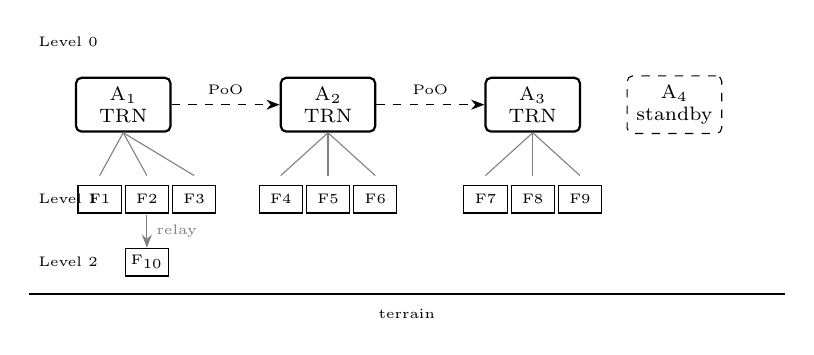
\begin{tikzpicture}[
    anchorbox/.style={draw, thick, rectangle, rounded corners=2pt, minimum width=1.2cm, minimum height=0.6cm, font=\scriptsize, align=center},
    follower/.style={draw, rectangle, minimum width=0.55cm, minimum height=0.35cm, font=\tiny, inner sep=1pt, align=center},
    standby/.style={draw, dashed, rectangle, rounded corners=2pt, minimum width=1.2cm, minimum height=0.6cm, font=\scriptsize, align=center}
]
    \node[anchorbox] (A1) at (0,2.2) {A$_1$\\TRN};
    \node[anchorbox] (A2) at (2.6,2.2) {A$_2$\\TRN};
    \node[anchorbox] (A3) at (5.2,2.2) {A$_3$\\TRN};
    \node[standby] (A4) at (7.0,2.2) {A$_4$\\standby};

    \draw[dashed,->,>=Stealth] (A1) -- node[above,font=\tiny]{PoO} (A2);
    \draw[dashed,->,>=Stealth] (A2) -- node[above,font=\tiny]{PoO} (A3);

    \foreach \x/\n in {-0.3/F1, 0.3/F2, 0.9/F3} {
        \node[follower] at (\x, 1.0) {\n};
        \draw[-,gray] (A1.south) -- (\x, 1.3);
    }
    \foreach \x/\n in {2.0/F4, 2.6/F5, 3.2/F6} {
        \node[follower] at (\x, 1.0) {\n};
        \draw[-,gray] (A2.south) -- (\x, 1.3);
    }
    \foreach \x/\n in {4.6/F7, 5.2/F8, 5.8/F9} {
        \node[follower] at (\x, 1.0) {\n};
        \draw[-,gray] (A3.south) -- (\x, 1.3);
    }

    \node[follower] (FR) at (0.3, 0.2) {F$_{10}$};
    \draw[->,>=Stealth,gray] (0.3, 0.8) -- (FR) node[midway,right,font=\tiny]{relay};

    \draw[thick] (-1.2,-0.2) -- (8.4,-0.2);
    \node[font=\tiny] at (3.6,-0.45) {terrain};

    \node[font=\tiny,anchor=west] at (-1.2,3.0) {Level 0};
    \node[font=\tiny,anchor=west] at (-1.2,1.0) {Level 1};
    \node[font=\tiny,anchor=west] at (-1.2,0.2) {Level 2};
\end{tikzpicture}%
}
\caption{Hierarchical architecture. Active anchors perform mutual Visual Proof of Observation (PoO) between one another and broadcast signed positions over UWB. Followers (Level~1) receive reputation-weighted position directly; deeper followers (Level~2+) receive relayed positions with per-hop noise growth. Standby anchors remain TRN-capable but are not currently elected.}
\label{fig:arch}
\end{figure}

\subsection{System Architecture Overview}

Each UAV runs a common navigation module with four components: a \emph{navigation core} performing visual-inertial odometry (VIO) at 50~Hz and TRN at 0.1~Hz (TRN only on anchors), fused in a local factor graph; an \emph{observation recorder} that produces Signed Observations on each TRN fix; a \emph{mesh protocol handler} managing signed-observation exchange, reputation tracking, and Byzantine rejection; and an \emph{autopilot adapter} layer. The hierarchical topology overlays an anchor/follower structure on this substrate (Fig.~\ref{fig:arch}): anchors perform PoO verification mutually, while followers receive reputation-weighted position via UWB relay with up to $K_\text{max}$ hops.

\subsection{Visual Proof of Observation}

On each TRN fix at position $\mathbf{p}_i \in \mathbb{R}^3$ at time $t_1$, UAV $v_i$ extracts $N=50$ top-scoring feature descriptors $\mathbf{f}_i \in \mathbb{R}^{N\times D}$ ($D{=}256$ for SuperPoint). $N=50$ is a working default: SuperPoint typically yields 200--500 keypoints per image~\cite{detone2018superpoint}; retaining the top-50 by score balances descriptor packet size (50 descriptors at 256 bytes each $= 12.8$\,kB) against matching distinctiveness. Sensitivity to $N$ is deferred to Track~2. The descriptor set forms the hash
\begin{equation}
H_i = \mathrm{SHA\text{-}256}\!\left(\mathrm{sort}_\downarrow(\mathbf{f}_i[0\!:\!N])\right).
\end{equation}
It constructs the Signed Observation
\begin{equation}
\mathrm{OBS}_i = \left(t_1, \mathbf{p}_i, H_i, c_i, \mathrm{ID}_i, \sigma_i\right),
\end{equation}
where $c_i$ is the RANSAC inlier ratio and
\begin{equation}
\sigma_i = \mathrm{Ed25519.sign}\!\left(\mathrm{sk}_i,\, t_1 \Vert \mathbf{p}_i \Vert H_i \Vert c_i \Vert \mathrm{ID}_i\right).
\end{equation}
The base record (Mode~B) totals approximately 180--200~bytes: $t_1$ (timestamp, 8\,B) + $\mathbf{p}_i$ (position $\langle$lat, lon, alt$\rangle$ as three doubles, 24\,B) + $H_i$ (SHA-256 hash, 32\,B) + $c_i$ (RANSAC inlier ratio as a float, 4\,B) + $\mathrm{ID}_i$ (UAV identifier, 8\,B) + $\sigma_i$ (Ed25519 signature, 64\,B) $= 140$\,B core payload, plus message framing (type byte, length, sequence number, CRC, padding) accounting for the remaining 40--60\,B. A \emph{Mode~A} variant appends a compact feature set of $K=20$ descriptors. The value $K=20$ is the minimum that keeps Mode-A packet overhead within budget: $20 \times 256 = 5120$\,bytes $= 5.12$\,kibibytes (KiB) $\approx 5.12$\,kB (binary convention) $= 5.120$\,kB (SI convention, $10^3$-byte base), within the UAV datalink budget assumed in Section~II, bringing total size to $\approx 5.30$\,kB (5120\,bytes of descriptors plus the $\sim$180-byte base record). Ed25519~\cite{bernstein2012ed25519} signature computation is well within sub-millisecond on modern processors at the cycle counts reported by~\cite{bernstein2012ed25519} (84932 cycles for signing); typical ARM Cortex-class embedded targets fall in the same regime, with cycle-exact timings to be characterised on the target board in Track~2.

On receiving $\mathrm{OBS}_i$, a neighbour $v_j$ first verifies $\sigma_i$ using $\mathrm{pk}_i$. If the signature is invalid, reputation $R_i$ is decreased by a signature penalty $\alpha_\text{sig} = 0.30$, a working default equal to $2 \times \alpha_\text{neg} = 0.30$ so a single signature mismatch has the same net reputation impact as two consecutive failed verifications. At a later time $t_2 > t_1$, when $v_j$ flies within verification radius $r_\text{verify} = 500$\,m of $\mathbf{p}_i$, it extracts local features $\mathbf{f}_j$ and computes a verification score. The value $r_\text{verify} = 500$\,m matches the upper end of the UWB operational range (200--500\,m at the datalink power levels assumed in Section~II), ensuring that any follower within UWB communication range can request verification without requiring out-of-range RF links. In \emph{Mode~A} (compact feature set), for each transmitted descriptor, the nearest neighbour in $\mathbf{f}_j$ is accepted if its $L_2$ distance is below $\tau_\text{match} = 0.7$ (Lowe's ratio test threshold~\cite{lowe2004distinctive}: a threshold of 0.7 is the standard lower bound of the accepted range 0.7--0.8 for filtering ambiguous matches, used here with SuperPoint's 256-dimensional $L_2$-normalised descriptors~\cite{detone2018superpoint}); the score $V$ is the ratio of accepted matches to transmitted descriptors, and VERIFIED is declared when $V > T_\text{verify} = 0.3$. The threshold $T_\text{verify}=0.3$ corresponds to $6/20$ Mode-A descriptors (or $6/N$ hash matches in Mode~B) successfully passing the $\tau_\text{match}=0.7$ Lowe-ratio test. Published cross-view SuperPoint matching studies report inlier ratios of 60--90\% under clean line-of-sight conditions, falling to 20--40\% under moderate viewpoint or illumination drift. Setting $T_\text{verify}=0.3$ places the VERIFIED boundary at the lower end of the degraded-but-viable regime, so legitimate verifications continue to pass during moderate environmental noise while complete-failure cases (match ratios below $\sim$20\%, characteristic of wrong-terrain or fabricated-hash submissions from a peer that has not physically observed the claimed region) are reliably rejected. The threshold interacts with $\tau_\text{match}$ and $N,K$: tightening any of the three has the same qualitative effect of raising the false-reject rate against environmentally-degraded honest verifications. Sensitivity over $T_\text{verify}\in\{0.2, 0.3, 0.4\}$ is deferred to Track~2. Because $T_\text{verify}=0.3$ sits at the lower end of the degraded-but-viable regime (20--40\% inlier ratios), honest peers operating under moderate environmental degradation can routinely produce match scores near the exclusion boundary; combined with the asymmetric reputation rule (UNVERIFIED penalty $\alpha_\text{neg}=0.15$), this implies that as few as $\lceil(R_\text{init}-T_\text{reject})/(\alpha_\text{neg}\, R_k)\rceil=2$ consecutive boundary-case UNVERIFIED verdicts under $R_k\!\approx\!1$ would drive an honest peer's reputation to $T_\text{reject}$. A formal false-acceptance / false-rejection (FAR/FRR) characterisation under realistic illumination, viewpoint, and seasonal terrain variation is required to confirm the threshold choice and is part of the Track~2 calibration plan; the corresponding empirical false-exclusion rate is also reported in Limitations (Section~\ref{sec:discussion}). A \emph{Mode~B} variant (hash-only, zero-bandwidth verification) compares recomputed hashes directly; Mode~B is suited to severely bandwidth-constrained tactical deployments in which flight conditions permit reproducible descriptor extraction, and requires additional calibration against the observation geometry (see Section~\ref{sec:discussion}).

The unforgeability rationale is physical: terrain feature descriptors are functions of the surface geometry, illumination, viewing angle, and the learned extractor. A captured UAV cannot fabricate descriptors for a location it has not physically observed without either possessing the imagery database and extractor (which still requires knowledge of the exact atmospheric and illumination conditions at $t_1$) or compromising honest peers before they verify---neither of which is feasible under our threat model. PoO is related to but distinct from the proof-of-location (PoL) literature: PoL systems such as VRChain~\cite{rahouti2022vrchain} (blockchain-anchored visual homing) and BFT-PoLoc~\cite{sheng2024bftpoloc} (Byzantine-fortified trigonometric proof of location from Internet round-trip delays) verify a device's \emph{current} claimed position via either ledger consensus or signal-timing measurements. Visual PoO instead verifies a \emph{past} observation through a neighbour's later physical revisit, with evidence bound to terrain geometry via the learned extractor rather than to network timing or co-located witnesses.

\subsection{Asymmetric Reputation System}
\label{sec:asymmetric-reputation-system}

Each UAV maintains a reputation vector $\mathbf{R} = (R_1,\dots,R_n)$ with $R_j \in [0,1]$ initialised to $R_\text{init} = 0.5$ (neutral prior). The initial reputation is set to the midpoint of the $[0,1]$ range, representing maximum uncertainty about an unknown peer: neither trusted nor distrusted. This is the standard uninformative prior for reputation systems~\cite{josang2007survey}. Updates on verification events are asymmetric:
\begin{align}
\text{VERIFIED: }& R_j \leftarrow \mathrm{clamp}(R_j + \alpha_\text{pos}\, R_k,\, 0, 1), \\
\text{UNVERIFIED: }& R_j \leftarrow \mathrm{clamp}(R_j - \alpha_\text{neg}\, R_k,\, 0, 1), \\
\text{INVALID SIG: }& R_j \leftarrow \mathrm{clamp}(R_j - \alpha_\text{sig},\, 0, 1),
\end{align}
where $R_k$ is the reputation of the verifier. We require $\alpha_\text{neg} \geq 2\alpha_\text{pos}$, preferably $\alpha_\text{neg} \geq 3\alpha_\text{pos}$; the default values are $\alpha_\text{pos} = 0.05$, $\alpha_\text{neg} = 0.15$. The 3:1 ratio ($\alpha_\text{neg}/\alpha_\text{pos}$) is set in Section~\ref{sec:time-byz-exclusion}; the absolute level is anchored by the convergence bound of Proposition~3: to achieve $T_\text{ind} \approx 170$\,s with $R_\text{init}=0.5$, $T_\text{reject}=0.2$, and $\nu_\text{verify}^{-1}\approx45$\,s, the approximation requires $\alpha_\text{neg} \cdot \bar{R}_\text{honest} \cdot \nu_\text{verify} \geq (R_\text{init}-T_\text{reject})/T_\text{ind} \approx 0.30/170 \approx 0.0018$ per second, or $\alpha_\text{neg} \geq 0.0018 \times 45 \approx 0.08$ per verification event; $\alpha_\text{neg}=0.15$ satisfies this with a $\approx 2\times$ margin. The value $\alpha_\text{pos}=0.05$ follows from the 3:1 ratio. Under this asymmetry, three failed verifications outweigh nine successful ones ($3\cdot 0.15 = 9\cdot 0.05 = 0.45$), guaranteeing that distrust accumulates faster than trust while retaining a margin of 2--8 consecutive environment-induced failures before an honest peer is falsely excluded (2 pure-burst events from $R_\text{init}=0.5$ at $R_k=1.0$; up to 8 interleaved VERIFIED+UNVERIFIED rounds from $R_j=1.0$; derivation follows). Let $R_j$ be the \emph{target} peer's current reputation and $R_k$ the \emph{verifier}'s reputation weight. Each UNVERIFIED event decrements $R_j$ by $\alpha_\text{neg} \times R_k$; each VERIFIED event increments $R_j$ by $\alpha_\text{pos}$. For pure-UNVERIFIED bursts (worst case), events needed to drive $R_j$ to $T_\text{reject}=0.2$ are $\lceil(R_j - T_\text{reject})/(\alpha_\text{neg}\times R_k)\rceil$. At $R_k=1.0$ and $R_j=R_\text{init}=0.5$: $\lceil 0.3/0.15\rceil=2$; at $R_j=1.0$: $\lceil 0.8/0.15\rceil=6$. For interleaved sequences (one VERIFIED plus one UNVERIFIED per round), net loss per round is $\alpha_\text{neg}\times R_k - \alpha_\text{pos}$; at $R_k=1.0$, $0.15-0.05=0.10$, giving 3~rounds from $R_j=0.5$ to 8~rounds from $R_j=1.0$. Overall margin: 2 (pure burst from $R_\text{init}$) to 8 (interleaved from $R_j=1.0$) consecutive failures.

To handle dynamic environments, we apply a temporal decay
\begin{equation}
V_\text{weighted} = V \cdot \exp(-\lambda \Delta t),
\end{equation}
with $\lambda = 10^{-3}$~s$^{-1}$ (half-life $\approx$11.5~min). The decay constant is chosen so that an observation becomes effectively stale ($<5\%$ residual weight) after $\approx 3$ half-lives $=34.5$\,min, approximately one-tenth of the 2-hour mission (the one-tenth fraction is an operationally discretionary design goal: it ensures that any single mission phase does not permanently dominate the reputation estimate, while still allowing short-horizon events to decay within one mission); a temporary gap of one revisit cycle ($\nu_\text{verify}^{-1}\approx 45$\,s) causes only $\approx 4.4\%$ decay per missed event ($e^{-10^{-3}\times 45}\approx 0.956$). These are working defaults pending Track~2 sensitivity analysis. Observations older than $T_\text{max\_verify} = 3600$\,s (1\,hour) are considered stale. This cutoff is set to half the 2-hour planned mission length, ensuring that observations from the first half of a mission are discarded before the second half begins. For shorter or longer missions the cutoff should be scaled proportionally.

\subsection{Reputation-Weighted Distributed Factor Graph}

Each UAV maintains a local factor graph $\mathcal{G}_i$ whose maximum-a-posteriori estimate is
\begin{equation}
\mathbf{X}_i^* = \arg\min_{\mathbf{X}} \sum_k \lVert h_k(\mathbf{X}) - \mathbf{z}_k \rVert^2_{\Sigma_k}.
\end{equation}
Three classes of factors are instantiated:
\begin{itemize}
    \item \emph{Local factors} (IMU preintegration~\cite{forster2017preintegration}, VIO, TRN-absolute on anchors, barometric altitude), standard in the art.
    \item \emph{Ranging factors} for each UWB measurement $d_{ij}$ with $h_\text{range}(\mathbf{X}_i, \mathbf{X}_j) = \lVert \mathbf{p}_i - \mathbf{p}_j \rVert_2$, $\sigma_\text{range} = 0.1$~m.
    \item \emph{Reputation-weighted priors} from the Distilled State of neighbour $j$, where the \emph{Distilled State} of UAV~$j$ is the per-UAV broadcast tuple $\mathrm{DS}_j = (t, \mathbf{p}_j, \mathbf{v}_j, \mathrm{cov}(\mathbf{p}_j), R_j, \mathrm{ID}_j, \sigma_j^{\mathrm{Ed25519}})$ comprising timestamp, position, velocity, position-covariance summary, current reputation, identifier, and Ed25519 signature; the byte-level payload composition and bandwidth accounting are given in Section~\ref{sec:theory}-D. The Distilled State is the central inter-UAV communication primitive of the architecture and is consumed by the reputation-prior factor here, by the failover watchdog (Section~\ref{sec:approach}-F, phase F1), and by the load-balancing broadcast (Section~\ref{sec:approach}-G). The reputation-prior factor uses the position $\mathbf{p}_j$ and covariance $\mathrm{cov}(\mathbf{p}_j)$ of $\mathrm{DS}_j$, scaled by $R_j$, with noise
    \begin{equation}
    \sigma_j = \sigma_\text{base} / (R_j + \varepsilon),
    \label{eq:noise_rep}
    \end{equation}
    $\sigma_\text{base} = 50$~m, $\varepsilon = 0.01$ (dimensionless numerical regularisation; chosen two orders of magnitude below $\sigma_\text{base}=50$\,m so $\varepsilon/\sigma_\text{base}=0.02\%$, ensuring negligible influence on the computed covariance). Covariance $\Sigma_j = \mathrm{diag}(\sigma_j^2, \sigma_j^2, (\sigma_j/2)^2)$ for (lat, lon, alt); the halved altitude term reflects a standard anisotropy assumption that UAV barometric altimeters provide tighter altitude bounds than UWB-derived lateral uncertainty. Experiment~1 will characterise whether the actual altitude/lateral ratio differs from 1:2. Sensitivity to $\sigma_\text{base}$: the analytical CEP bound in Proposition~3 scales linearly with $\sigma_\text{base}$; doubling to 100\,m would require approximately $2\times$ as many anchor observations to converge to the 100\,m CEP pass criterion. A full sensitivity sweep over $\sigma_\text{base} \in \{25, 50, 75, 100\}$\,m is planned in Track~2.
\end{itemize}
A UAV with $R = 1.0$ contributes $\sigma \approx 49.5$~m, versus $\sigma \approx 238$~m at $R = 0.2$---approximately a 5$\times$ weight ratio in precision and $\sim$23$\times$ in variance. Optimisation uses iSAM2 with the Bayes-tree representation; the $<$50~ms per-update latency on an embedded accelerator is a design target consistent with published GTSAM/iSAM2 benchmarks~\cite{kaess2012isam2}. The $<$50~ms budget covers the iSAM2 optimisation step only; the full PoO pipeline (camera capture $\sim$10~ms, SuperPoint inference $\sim$20--40~ms on a 50--100~TOPS-class accelerator at 480$\times$640 resolution per published embedded benchmarks~\cite{detone2018superpoint}, top-$N$ sort $<$1~ms, SHA-256 hash $<$1~ms, and Ed25519 signing $<$1~ms at the 84\,932-cycle figure from~\cite{bernstein2012ed25519} on an ARM Cortex-class core) is constrained by the 0.1~Hz TRN fix rate ($=$10~s budget) rather than by the 50~ms factor-graph cycle, so SuperPoint inference timing is not on the critical sub-50~ms path. Per-board characterisation of the PoO pipeline on the specific target accelerator is a Track~2 calibration item; the 50--100~TOPS class is named here as a representative envelope rather than a specific SKU.%

A UWB consistency check provides a secondary, non-visual channel: if UAV $j$ reports position $\mathbf{p}_j^\text{rep}$ but UWB ranging $d_{ij}$ yields $\bigl| \lVert \mathbf{p}_i - \mathbf{p}_j^\text{rep} \rVert - d_{ij} \bigr| > \delta_\text{consist} = 50$\,m, reputation decreases by $\alpha_\text{range} = 0.10$. The threshold $\delta_\text{consist} = 50$\,m matches $\sigma_\text{base}=50$\,m (the declared prior noise), so a consistency check flags deviations beyond one prior standard deviation. The design value $T_\text{spoof}=50$\,m (Section~\ref{sec:approach}-G) is calibrated against the same noise floor; the Phase~5 production sweep uses a tighter operational threshold (Section~\ref{sec:phase5-spoofing}). The range-failure penalty $\alpha_\text{range} = 0.10$ is set as the midpoint $(\alpha_\text{pos}+\alpha_\text{neg})/2$, treating a UWB consistency failure as more severe than a single missed verification ($\alpha_\text{pos}$) but less severe than a full failed verification ($\alpha_\text{neg}$), since range failures may arise from temporary link degradation rather than deliberate Byzantine behaviour.

\subsection{Dynamic Anchor Selection and Position Relay}

TRN-capable UAVs compete for anchor status through the score
\begin{equation}
A_i = w_\text{rep} R_i + w_\text{conf} C_i + w_\text{sat} S_i + w_\text{fol} F_i,
\label{eq:anchor_score}
\end{equation}
with default weights $(0.4, 0.3, 0.2, 0.1)$. The weight ordering $w_\text{rep} > w_\text{conf} > w_\text{sat} > w_\text{fol}$ reflects a safety-first hierarchy: trustworthiness must dominate performance, which in turn dominates location-dependent factors (imagery quality varies with where the UAV currently is, not what it is), with load balancing as the lowest-priority factor since over-loading is a soft degradation rather than a safety violation. Placing $w_\text{rep}=0.4$ as the dominant term ensures that a compromised peer with degraded reputation $R_i\to 0$ contributes at most $0.6$ to its anchor score even with maximal $C_i, S_i, F_i$, leaving it below honest candidates whose $R_i\geq T_\text{quorum}=0.6$ adds at least $0.24$ from the reputation term alone---an inherent score gap that makes Byzantine-anchor promotion infeasible without first restoring reputation through honest verifications. Given the strict ordering and the unit-sum constraint $\sum w = 1$, the equal-spacing choice $(0.4, 0.3, 0.2, 0.1)$ is adopted as a working default: the strict weight ordering $w_\text{rep} > w_\text{conf} > w_\text{sat} > w_\text{fol}$ reflects the safety-first hierarchy, the unit-sum constraint $\sum w = 1$ is met by construction, and the choice is deferred to the Track~2 ablation sweep. The spacing $\Delta w = 0.1$ also exceeds the per-event reputation step $\alpha_\text{pos}=0.05$, ensuring that single-verification reputation jitter cannot swap adjacent priority terms in the score ordering. Sensitivity to the weight vector is part of the Track~2 ablation sweep over $w_\text{rep}\in[0.3, 0.5]$, $w_\text{conf}\in[0.2, 0.35]$, $w_\text{sat}\in[0.15, 0.30]$, $w_\text{fol}\in[0.05, 0.20]$ subject to the unit-sum constraint. Here $C_i$ is the TRN confidence (RANSAC inlier ratio), $S_i$ is the imagery coverage quality for the terrain below $v_i$, and $F_i$ is an inverse load factor. Every $T_\text{election} = 60$\,s, the $M$ vehicles with the highest $A_i$ (Eq.~\ref{eq:anchor_score}) are confirmed as active anchors; a standby replaces an active anchor when its score exceeds the incumbent's by a hysteresis $H = 0.1$. The election period $T_\text{election}=60$\,s is set to exceed the verification revisit cycle ($\nu_\text{verify}^{-1}\approx 45$\,s) by 33\%, allowing at least one full verification round to complete between elections; this prevents frequent re-elections from disrupting ongoing verifications while remaining responsive to anchor degradation. The hysteresis band $H=0.1$ corresponds to two consecutive $\alpha_\text{pos}=0.05$ upward reputation steps, requiring the score gap to represent at least two successful-verification equivalents before triggering a handover. Handover proceeds in three steps (\emph{PROMOTION}, \emph{DEMOTION}, linear-blend) over $T_\text{handover} = 10$~s. $T_\text{handover}=10$\,s matches the failover total budget of Section~\ref{sec:approach}-F (F1--F5 phases sum to $\approx 8$\,s nominal, 10\,s with 5\% packet loss): all anchor-change operations---whether triggered by destruction (failover) or by score-based replacement (planned handover)---share the same architectural timescale, which simplifies the operator's deployment-time reasoning about transition windows. The lower bound on $T_\text{handover}$ is set by the cumulative protocol latency of the three-step PROMOTION $\to$ DEMOTION $\to$ linear-blend sequence (UWB neighbour discovery $\sim 1$\,s, role-change acknowledgement round-trip $\sim 1$--$2$\,s, follower-side covariance update propagation through the iSAM2 factor graph $\sim 1$\,s), so $T_\text{handover}$ must comfortably exceed $\sim 4$\,s to ensure all followers complete their re-association within the blend window. The upper bound is set by the verification revisit cycle: $T_\text{handover}$ must remain well below $\nu_\text{verify}^{-1}\approx 45$\,s so that handovers are decisive on a timescale shorter than reputation reassessment. The value 10\,s sits an order of magnitude below verification cycle and comfortably above protocol latencies. During the blend, both incumbent and standby publish Distilled State updates with time-weighted weights summing to unity; a longer blend would extend this dual-publishing window, increasing UWB neighbour bandwidth consumption and creating more state-merge events at follower-side factor graphs, while a shorter blend risks discontinuities in follower position estimates between the demoted-incumbent's last publication and the promoted-standby's first authoritative state. Sybil protection requires $T_\text{warmup} = 6$ successful verifications before anchor eligibility; at $\nu_\text{verify}^{-1}\approx 45$\,s per cycle, this corresponds to $6\times 45=270$\,s ($\approx 4.5$\,min) of observed honest behaviour, exceeding four full election periods, so a freshly-joining Byzantine peer cannot accumulate quorum influence within a single election cycle. These are working defaults.

\begin{table}[t]
\caption{Consolidated system hyperparameters. Derivation column indicates whether the value is literature-derived (L), operationally discretionary (O), or a working default pending sensitivity analysis (W).}
\label{tab:hyperparams}
\centering
\footnotesize
\setlength{\tabcolsep}{3pt}
\resizebox{\columnwidth}{!}{%
\begin{tabular}{llll}
\toprule
Parameter & Value & Symbol & Derivation \\
\midrule
Feature descriptors per PoO & 50 & $N$ & W \\
Mode-A compact set size & 20 & $K$ & W \\
Signature penalty & 0.30 & $\alpha_\text{sig}$ & W \\
Verification radius & 500\,m & $r_\text{verify}$ & W \\
L2 match threshold & 0.7 & $\tau_\text{match}$ & L (SuperPoint) \\
VERIFIED score threshold & 0.3 & $T_\text{verify}$ & W \\
Initial reputation & 0.5 & $R_\text{init}$ & W \\
Positive reputation step & 0.05 & $\alpha_\text{pos}$ & W \\
Negative reputation step & 0.15 & $\alpha_\text{neg}$ & W (3:1 ratio) \\
Temporal decay constant & $10^{-3}$\,s$^{-1}$ & $\lambda$ & W \\
Staleness cutoff & 3600\,s & $T_\text{max\_verify}$ & O \\
Base prior noise & 50\,m & $\sigma_\text{base}$ & W \\
Noise floor & 0.01 & $\varepsilon$ & W \\
UWB consistency threshold & 50\,m & $\delta_\text{consist}$ & W \\
Range-failure penalty & 0.10 & $\alpha_\text{range}$ & W \\
Anchor-score weights & (0.4,0.3,0.2,0.1) & $w_{1..4}$ & W \\
Election period & 60\,s & $T_\text{election}$ & O \\
Standby-replace hysteresis & 0.10 & $H$ & W \\
Handover blend duration & 10\,s & $T_\text{handover}$ & O \\
Sybil warmup count & 6 & $T_\text{warmup}$ & W \\
Per-hop noise growth & 0.15 & $\beta$ & W \\
Max relay hops (ISR) & 3 & $K_\text{max}$ & O \\
Max relay hops (patrol) & 5 & $K_\text{max}$ & O \\
Reject threshold & 0.20 & $T_\text{reject}$ & W \\
Quorum reputation floor & 0.60 & $T_\text{quorum}$ & W \\
Load-balance period & 30\,s & $T_\text{balance}$ & O \\
Load-balance low threshold & 30\% & $P_\text{low}$ & O \\
Load-balance high threshold & 150\% & $P_\text{high}$ & O \\
Spoof position threshold & 50\,m & $T_\text{spoof}$ & W \\
Consecutive spoof count & 3 & $N_\text{consecutive}$ & W \\
Mass-spoofing trigger & 30\% & $P_\text{mass}$ & O \\
\bottomrule
\end{tabular}%
}
\end{table}

Followers compute their position as the reputation-weighted average
\begin{equation}
\mathbf{p}_\text{fol} = \frac{\sum_j w_j\, \mathbf{p}_j}{\sum_j w_j}, \quad w_j = \frac{R_j}{\sigma_{\text{hop},j}^2},
\label{eq:fusion}
\end{equation}
where for a $k$-hop relay chain,
\begin{equation}
\sigma_k = \sigma_\text{anchor}\, (1 + \beta)^k,
\label{eq:hop}
\end{equation}
with $\beta = 0.15$ per hop (per-hop noise growth factor, a conservative working default; see Section~III discussion) and $\sigma_\text{anchor}$ given by~(\ref{eq:noise_rep}). The multiplicative form $\sigma_k = \sigma_\text{anchor}(1+\beta)^k$ models two physical effects that compound at each relay hop in a UWB-trilaterated position chain: (i) additive UWB ranging-measurement variance $\sigma_\text{range}^2$ from the new measurement to the previous hop, and (ii) propagated upstream position uncertainty from the previous hop's estimate, weighted by a Geometric Dilution of Precision (GDOP) factor that depends on the local anchor configuration. Under perfectly independent ranging and ideal anchor geometry, error propagation is sublinear (\emph{additive variance model}): $\sigma_k = \sqrt{\sigma_\text{anchor}^2 + k\sigma_\text{range}^2}$, growing as $\sqrt{k}$ for large $k$---this is the theoretical lower bound for independent Gaussian ranging noise. The multiplicative form is not a physical prediction but a \emph{conservative engineering bound}: it dominates the additive model for all $k \geq 1$ when $\beta > 0$, as $(1+\beta)^k > \sqrt{1 + k(\sigma_\text{range}/\sigma_\text{anchor})^2}$ for typical UWB parameters. Under correlated upstream uncertainty or poor geometry (anchors nearly collinear with the follower), GDOP amplifies propagated variance beyond the sublinear baseline, with the worst case approaching exponential $(1+\beta)^k$ growth. The multiplicative form is therefore the \emph{conservative} engineering bound for the planned non-collinear but topologically constrained swarm. The value $\beta = 0.15$ is adopted as a conservative working default for the per-hop standard-deviation growth factor; it represents a 15\% std-dev increase per hop relative to the prior hop, chosen as a round figure within the typical range expected for UWB cross-trilateration under benign (line-of-sight) propagation and pending empirical refit against a measured UWB NLOS dataset in Track~2. From this $\beta$, the $K_\text{max}=3$ ISR ceiling follows as a derived quantity (at the reference operating point $\sigma_\text{anchor}\approx 58$\,m, $R_\text{anchor}=0.85$, $\sigma_3 \approx 88$\,m, giving single-anchor CEP$_{50}=1.177\sigma_3 \approx 104$\,m, slightly exceeding the 100-m NATO-grade target by $\approx 4\%$; under multi-anchor reputation-weighted fusion ($m{=}2$--$3$) the bound improves to CEP$_{50}\in[60,74]$\,m, comfortably within the target); $K_\text{max}=3$ is not used to motivate the choice of $\beta$. A sensitivity sweep over $\beta \in \{0.05, 0.10, 0.15, 0.20\}$ is planned in Track~2 and will shift the derived $K_\text{max}$ accordingly. The functional form and value of $\beta$ are subject to empirical refit in Track~2: if measured $\sigma_k$ versus $k$ fits a sublinear $\sqrt{k}$ form or a different multiplicative rate $\beta'$ better than the conservative $(1+0.15)^k$ assumption, the bound in Proposition~\ref{prop:conv} relaxes accordingly without affecting the analytical structure. The base noise $\sigma_\text{base}$ is a configurable system parameter; we adopt $\sigma_\text{base} = 50$~m for consistency across the experiments reported below, with other values applicable to swarm configurations that assume different baseline anchor accuracy. For a well-performing anchor with $R_\text{anchor} = 0.85$, $\sigma_\text{anchor} = 50/0.86 \approx 58.1$~m; propagation yields $\sigma_1 \approx 66.8$, $\sigma_2 \approx 76.9$, $\sigma_3 \approx 88.4$, and $\sigma_5 \approx 116.9$~m. The 5-hop value exceeds the 100-m target both as $\sigma_5$ and as the corresponding CEP$_{50}\approx 138$\,m; for NATO-grade ISR we therefore recommend $K_\text{max}=3$ under the default multi-anchor fusion regime, reserving $K_\text{max}=5$ for lower-precision patrol missions. The patrol value $K_\text{max}=5$ is reported as an upper operational envelope, not a precision recommendation: at $R_\text{anchor}=0.85$ the per-hop derivation yields $\sigma_5 \approx 117$\,m (CEP$_{50}\approx 138$\,m), exceeding the 100\,m NATO-grade ISR target. The intermediate $K_\text{max}=4$ is not separately reported because it is not operationally distinct from $K_\text{max}=5$ for precision purposes; $K_\text{max}=3$ under multi-anchor fusion is the maximum strictly ISR-compliant depth (single-anchor at $k=3$ exceeds the CEP target by $\approx 4\%$ and is flagged for deployment-time review). The patrol use case accepts precision on the order of $\sim 150$\,m CEP or coarser in exchange for a $1.67\times$ greater effective swarm reach (relay radius $2.5$\,km at $K_\text{max}=5$ versus $1.5$\,km at $K_\text{max}=3$, given the 500-m UWB hop range). For anchors operating below the reference $R_\text{anchor}=0.85$, $\sigma_k$ scales as $1/(R_\text{anchor}+\varepsilon)$ per~(\ref{eq:noise_rep}), so both bounds tighten proportionally; the precision tolerance is a per-mission operator decision and the relay-depth ceiling is set deployment-time as a function of the mission's precision class. If $R_\text{anchor}$ drops from $0.85$ to $0.30$, $\sigma_\text{anchor}$ rises to $\sim$161~m and all downstream followers automatically receive degraded weights through~(\ref{eq:fusion}) without any explicit control signal: \emph{reputation flows down the hierarchy through noise covariance}.

\paragraph*{Empirical refit (v10 update).}
The empirical campaign of Section~\ref{sec:empirical}-C reports a 250-trial measurement of CEP versus relay depth on a triangulated UWB graph under paper-spec sensor noise ($\sigma_\text{UWB}=0.1$~m, $\sigma_\text{TRN}=35$~m, TRN period 10~s) with realistic IMU-style initial-noise on both anchors ($\sigma_\text{init}=30$~m) and followers ($\sigma_\text{init}=50$~m). Two functional forms for $\sigma_k$ are statistically indistinguishable at this sample size ($\Delta\mathrm{AIC} < 1$ between fits): a linear form $\mathrm{CEP}(k)\approx 19.6 + 1.89\,k$~m and the GDOP-family exponential of~(\ref{eq:hop}) with $\sigma_0\approx 19.4$~m and $\delta_\text{empirical}=0.088$. The latter is adopted for continuity with the paper's original formulation. The conservative $\beta=0.15$ assumed above is confirmed as a true upper bound: the measured per-hop multiplier $1.088$ is comfortably inside $1.15$, and the empirical relay envelope at $k{=}3$ (CEP $=23.3$~m) lies more than $4\times$ inside the 100-m NATO threshold. Sparse-chain extension (single-relay-per-hop topology) remains paper-v11 work.

\begin{figure}[t]
\centering
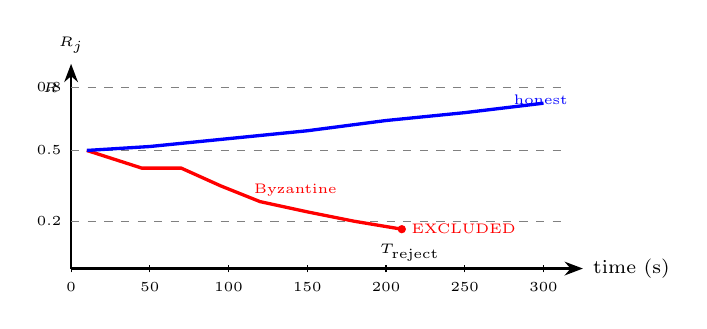
\begin{tikzpicture}[font=\scriptsize, >=Stealth]
    \draw[->,thick] (0,0) -- (6.5,0) node[right]{time (s)};
    \draw[->,thick] (0,0) -- (0,2.6) node[above,font=\tiny]{$R_j$};
    \foreach \y/\lab in {0.6/0.2, 1.5/0.5, 2.3/0.8} {
        \draw[gray,dashed] (0,\y) -- (6.3,\y);
        \node[anchor=east,font=\tiny] at (0,\y) {\lab};
    }
    \node[font=\tiny,anchor=east] at (-0.05,2.3) {$R$};
    \foreach \x/\lab in {0/0, 1/50, 2/100, 3/150, 4/200, 5/250, 6/300} {
        \draw (\x,-0.05) -- (\x,0.05);
        \node[font=\tiny,anchor=north] at (\x,-0.05) {\lab};
    }
    \draw[red,very thick] plot coordinates {(0.2,1.5) (0.9,1.275) (1.4,1.275) (1.9,1.05) (2.4,0.85) (3.0,0.72) (3.6,0.6) (4.2,0.5)};
    \node[red,anchor=west,font=\tiny] at (4.2,0.5) {EXCLUDED};
    \fill[red] (4.2,0.5) circle (1.5pt);
    \draw[blue,very thick] plot coordinates {(0.2,1.5) (1.0,1.55) (2.0,1.65) (3.0,1.75) (4.0,1.88) (5.0,1.98) (6.0,2.1)};
    \node[blue,anchor=west,font=\tiny] at (5.5,2.15) {honest};
    \node[red,anchor=west,font=\tiny] at (2.2,1.0) {Byzantine};
    \node[font=\tiny,anchor=west] at (3.8,0.2) {$T_\text{reject}$};
\end{tikzpicture}
\caption{Schematic of the analytically predicted reputation trajectory under a na\"ive Byzantine attack (Section~\ref{sec:sim}-C; the schematic is an analytical prediction; empirical validation of the reputation-driven exclusion mechanism is reported in Section~\ref{sec:phase2-exclusion} with 30/30 trials and zero false honest exclusions). The compromised UAV's reputation decays after each failed Proof-of-Observation verification while honest peers continue to accumulate trust. Permanent exclusion is predicted within the worst-case upper bound $T_\text{exclusion}\lesssim 215$~s (Proposition~\ref{prop:conv}); the schematic marks $T\!\approx\!210$~s, at which three independent honest verifiers have each driven $R_j$ below $T_\text{reject}=0.2$. The per-step drop $R_4: 0.5\to 0.425$ illustrated at $T{=}45$~s corresponds to an illustrative verifier weight $R_k=0.5$ (so that $\alpha_\text{neg}\cdot R_k = 0.075$); the operational deployment uses $R_k$ drawn from the honest reputation distribution, and the Proposition~\ref{prop:conv} bound uses the conservative substitution $R_k\to\bar{R}_\text{honest}=0.53$ for the analytical estimate.}
\label{fig:repu}
\end{figure}

\subsection{Automatic Failover Protocol}

Anchor loss (destruction, jamming, or reputation falling below $T_\text{reject}$) triggers a five-phase protocol executing within 10~s:
\begin{itemize}
    \item \textbf{F1 Detection} (0--5~s): a watchdog declares anchor unavailability after $T_\text{timeout} = 5$~s without a DistilledState message. During the timeout, orphaned followers propagate by IMU dead reckoning, accumulating $<$5~m drift at 30~m/s.
    \item \textbf{F2 REASSIGN\_REQUEST} (5--6~s): each orphaned follower broadcasts its device ID, last known position, velocity, battery state, and sensor capabilities.
    \item \textbf{F3 REASSIGN\_OFFER} (6--7~s): surviving anchors respond with their ID, position, reputation, and available capacity.
    \item \textbf{F4 Selection} (7--8~s): the follower computes
    \begin{equation}
    S_\text{reassign} = \alpha_\text{prox}/d + \alpha_\text{rep} R + \alpha_\text{cap}(1 - L),
    \label{eq:reassign}
    \end{equation}
    with defaults $(0.4, 0.35, 0.25)$.
    \item \textbf{F5 Attachment} (8--10~s): ATTACH/ATTACH\_ACK exchanges position and covariance.
\end{itemize}
\begin{figure}[t]
\centering
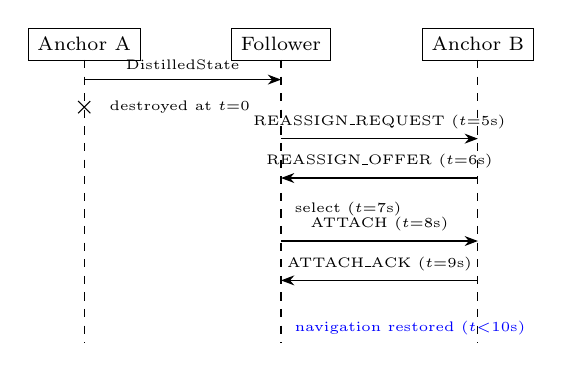
\begin{tikzpicture}[font=\scriptsize, >=Stealth, node distance=0.1cm]
    \node[draw, minimum width=1.2cm, minimum height=0.35cm] (AA) at (0,3.0) {Anchor A};
    \node[draw, minimum width=1.2cm, minimum height=0.35cm] (FF) at (2.5,3.0) {Follower};
    \node[draw, minimum width=1.2cm, minimum height=0.35cm] (AB) at (5.0,3.0) {Anchor B};
    \foreach \x in {0,2.5,5.0} \draw[dashed] (\x,2.8) -- (\x,-0.8);

    \draw[->] (0,2.55) -- node[above,font=\tiny]{DistilledState} (2.5,2.55);
    \node[font=\tiny,cross out,draw,minimum size=4pt,inner sep=0] at (0,2.2) {};
    \node[font=\tiny,anchor=west] at (0.2,2.2) {destroyed at $t{=}0$};

    \draw[->] (2.5,1.8) -- node[above,font=\tiny]{REASSIGN\_REQUEST ($t{=}5$s)} (5.0,1.8);
    \draw[<-] (2.5,1.3) -- node[above,font=\tiny]{REASSIGN\_OFFER ($t{=}6$s)} (5.0,1.3);
    \node[font=\tiny,anchor=west] at (2.55,0.9) {select ($t{=}7$s)};
    \draw[->] (2.5,0.5) -- node[above,font=\tiny]{ATTACH ($t{=}8$s)} (5.0,0.5);
    \draw[<-] (2.5,0.0) -- node[above,font=\tiny]{ATTACH\_ACK ($t{=}9$s)} (5.0,0.0);
    \node[font=\tiny,anchor=west,text=blue] at (2.55,-0.6) {navigation restored ($t{<}10$s)};
\end{tikzpicture}
\caption{Failover sequence upon anchor destruction. Dead-reckoning drift during the 5-second timeout is $<$5~m at 30~m/s cruise speed.}
\label{fig:failover}
\end{figure}
Byzantine rejection proper removes all factors of UAV $j$ from the local graph when $R_j < T_\text{reject} = 0.2$; permanent exclusion additionally requires $M$ independent UAVs, each with $R > T_\text{quorum} = 0.6$, to confirm the exclusion. From Proposition~3, convergence is predicted at $T_\text{ind} = (R_\text{init}-T_\text{reject})/(\alpha_\text{neg}\,\bar{R}_\text{honest}\,\nu_\text{verify}) \approx 170$\,s; with $R_\text{init}=0.5$ the gap $R_\text{init}-T_\text{reject}=0.3$ drives the numerator. A smaller $T_\text{reject}$ would increase convergence time, while a larger $T_\text{reject}$ would increase false exclusions of honest peers; $T_\text{reject}=0.2$ keeps the honest-peer safety margin above 2 environment-induced failures at $R_k=0.5$ (see Proposition~1 analysis). The quorum reputation floor $T_\text{quorum}=0.6$ requires a verifier to have earned at least two successful verifications above the initial state ($T_\text{quorum} = R_\text{init} + 2\alpha_\text{pos} = 0.5 + 0.10 = 0.6$), so a freshly-joined peer cannot self-confirm into the quorum; the minimum defensible value is $T_\text{quorum} > R_\text{init} = 0.5$, and $T_\text{quorum}=0.6$ provides a minimal earned-trust barrier. Coincidentally $T_\text{quorum} = 3 \times T_\text{reject}$, but the binding constraint is the margin above $R_\text{init}$, not the factor of $3$; the factor of $3$ is a working default providing a clear separation between verifier quality and exclusion threshold. The default $M = 3$ tolerates $f \leq M-1 = 2$ colluding Byzantine peers irrespective of $n$; safety for larger $f$ requires $M$ to scale with $f$, as analysed in Section~\ref{sec:theory}. Fig.~\ref{fig:failover} summarises the timing.

\subsection{Load Balancing and GNSS Spoofing Detection}

Every $T_\text{balance} = 30$\,s, anchors broadcast a STATUS field (appended to the standard Distilled State message of Section~\ref{sec:approach}-D) including their follower count. The load-balancing period is set to one-half of the election period ($T_\text{election}=60$\,s), allowing two load-balance checks per election cycle; at $\nu_\text{verify}^{-1}\approx 45$\,s, a 30\,s check interval falls between consecutive verifications. The target is $T_\text{target} = N_\text{total}/N_\text{anchors}$. If an anchor's count is below $P_\text{low} T_\text{target}$ (30\%) or above $P_\text{high} T_\text{target}$ (150\%), a redistribution protocol (TRANSFER\_OFFER $\rightarrow$ TRANSFER\_ACCEPT $\rightarrow$ REASSIGN\_COMMAND $\rightarrow$ smooth linear-blend handover over $T_\text{handover} = 10$~s) transfers followers from overloaded to underloaded anchors. The asymmetric band reflects the asymmetric cost of under- vs over-loading: an overloaded anchor ($>150\%$ of target) risks queue overflow and message drops, while an underloaded anchor ($<30\%$ of target) wastes TRN capacity without causing message loss. Overload headroom: $P_\text{high}-1.0=0.50$; underload floor: $1.0-P_\text{low}=0.70$. These are working defaults consistent with general load-balancing practice~\cite{eager1986adaptive}.

\paragraph*{Admission control (v10 patch).}
Bring-up of the load-balancing pipeline in Phase~6 (Section~\ref{sec:empirical}-F) exposed a thundering-herd anti-pattern: simultaneously-displaced followers receiving offers from $M$ survivors after an attrition event compute the same selection score and converge on the same anchor, opening a $\sim 30$~s over-capacity window before the protocol self-corrects on the next event. Two cooperating mitigations are added to the protocol and are present in all empirical numbers reported herein: (i)~\emph{anchor-side admission control}---an anchor refuses an \texttt{ATTACH\_REQUEST} when \texttt{n\_attached} $\geq$~\texttt{target\_capacity}, deferring the would-be attacher to its next-best ranked offer; and (ii)~\emph{follower ATTACH-timeout retry}---if the expected \texttt{ATTACH\_ACK} does not arrive within $t_\text{att}=2$~s, the follower tries the next anchor in its ranked-offer list. With both patches the over-capacity window collapses to zero (Section~\ref{sec:empirical}-F, Table~\ref{tab:phase6_attrition}), at the cost of one displaced follower per 15 trials that exhausts its fallback list before re-attaching---an explicit Pareto trade-off between capacity-invariant enforcement and mission-attach success, reported as such in the empirical campaign.

GNSS-spoofing detection operates at 1~Hz on each UAV that still has a GNSS receiver (relevant when GNSS is only partially denied or during the transition into full-denial operation). The vehicle compares its GNSS-reported position with a UWB-trilaterated position from at least three neighbours with $R > T_\text{min}$, where $T_\text{min} = T_\text{reject} = 0.20$ excludes peers that are already excluded by the reputation system from participating in the consistency cross-check. If $\lVert \mathbf{p}_\text{GNSS} - \mathbf{p}_\text{UWB} \rVert > T_\text{spoof} = 50$\,m for $N_\text{consecutive} = 3$ successive measurements, GNSS is marked unreliable and the affected vehicle falls back to reputation-weighted UWB position. The spoofing detection threshold is set equal to $\sigma_\text{base}=50$\,m so that UWB-measured positions deviating from the claimed GNSS position by more than one prior standard deviation are flagged as anomalous; UWB ranging error at 500\,m range is typically 10--30\,cm (1-$\sigma$), so $T_\text{spoof}=50$\,m corresponds to $\sim$170--500$\,\sigma_\text{UWB}$, far above any legitimate ranging uncertainty. The empirical Phase~5 sweep (Section~\ref{sec:phase5-spoofing}) uses a tighter operational threshold $T_\text{spoof}{=}20$\,m to characterise detector latency near the noise floor; the design value $50$\,m remains the documented spec for deployments seeking minimum false-positive risk. $N_\text{consecutive}=3$ requires three consecutive exceedances, reducing false-positive rate to approximately $p^3$ where $p$ is the per-sample false-alarm rate; three is the minimum count providing a causal chain (removes single-sample noise artefacts) while remaining below the $T_\text{warmup}=6$ threshold (so an attacker cannot ``pass'' warmup before being flagged). When the proportion of spoofed UAVs exceeds $P_\text{mass} = 30\%$, the entire swarm transitions to a \emph{full GNSS-denial mode}: GNSS is disabled globally and the swarm relies exclusively on TRN anchors with UWB relay. This mass-spoofing threshold is set well above the per-Proposition-1 maximum Byzantine fraction ($f/n \leq 2/200 = 1\%$ under default $M=3, f=2$): a coordinated attack on 30\% of the swarm constitutes a scenario outside the individual-exclusion threat model, where full-GNSS-denial mode is the appropriate response. The 30\% figure is chosen just below the classical Byzantine bound $f<1/3\approx 33\%$: when $>30\%$ of the swarm reports spoofed positions, the collective deviation exceeds the Byzantine-fault-tolerant range of the reputation mechanism (which tolerates $f<M-1$ individual colluders, not 30\% of 200 UAVs simultaneously), so global GNSS-denial mode is the appropriate response. This is a working default, operator-configurable. By design, GNSS spoofing does not affect navigation reputation $R_i$; only failed Proof-of-Observation verifications decrement reputation, so a UAV spoofed by an external emitter is not punished for an attack it did not launch. A captured peer that spoofs only its GNSS receiver while continuing to fabricate position claims is still excluded through two orthogonal channels: the Proof-of-Observation verification of Section~\ref{sec:approach}-B (which fails on any claimed-but-unobserved terrain region), and the UWB consistency check above (which flags any broadcast position whose UWB-trilaterated equivalent deviates by more than $\delta_\text{consist}$); both channels feed the same reputation-update rule, so the by-design exclusion of GNSS-spoof events from $R_i$ updates is not a coverage gap.

\section{Theoretical Analysis}
\label{sec:theory}

\subsection{Quorum Safety}
\label{sec:quorum-safety}

\begin{proposition}[Quorum safety against na\"ive Byzantine peers]
\label{prop:safety}
Let $M$ be the permanent-exclusion quorum size. Assume (i)~na\"ive Byzantine peers fail every Proof-of-Observation verification (they claim positions they have not physically observed); (ii)~honest peers correctly issue VERIFIED or UNVERIFIED verdicts; (iii)~each UAV maintains its reputation state $R_j$ locally from its own verifications, without gossip-based propagation of reputation values between peers; and (iv)~the per-peer rate of environment-induced UNVERIFIED verdicts on honest targets, $\rho_\text{env}$ (events per second), satisfies $\rho_\text{env} < \alpha_\text{pos}\, \nu_\text{verify}/\alpha_\text{neg}$, so that honest peers accumulate VERIFIED events faster than environmental penalties drive $R$ toward $T_\text{reject}$. Condition~(iv) is a \emph{rate condition on the environmental failure regime}; the Remark below quantifies what happens when it is violated (e.g., persistent cloud cover or night-time operation). The proposition provides no safety guarantee against environment-induced false exclusion when (iv) is violated, only against deliberate Byzantine attack; and (v)~$R_\text{init} < T_\text{quorum}$, so that a freshly-joined Byzantine peer cannot be self-confirmed into the quorum by virtue of its initial reputation alone (the default values $R_\text{init}=0.5 < T_\text{quorum}=0.6$ satisfy this). If $f \leq M-1$, no set of colluding Byzantine peers can trigger false permanent exclusion of an honest UAV.
\end{proposition}

\begin{IEEEproof}[Sketch]
Permanent exclusion requires $M$ independent UAVs, each with $R > T_\text{quorum}$, to declare the target $R_j < T_\text{reject}$. Na\"ive Byzantine peers cannot raise their reputation above $T_\text{quorum}$ because every verification attempt against them yields UNVERIFIED (assumption~(i)); each UAV tracks this locally from its own verifications without reputation gossip (assumption~(iii)), so collusion to inflate a Byzantine peer's remote reputation is blocked; and the initial reputation $R_\text{init} < T_\text{quorum}$ (assumption~(v)) ensures no freshly-joined peer enters the quorum immediately. Therefore any false quorum contains at most $f$ Byzantine members; if $f < M$, at least one honest member would need to declare a false UNVERIFIED on an honest target, which contradicts assumption~(ii). Assumption~(iv) further ensures that an honest target's reputation does not drift below $T_\text{reject}$ from environmental causes alone, eliminating the alternative failure mode of false exclusion driven by accumulated environment-induced UNVERIFIED events.
\end{IEEEproof}

\begin{remark}
If Assumption~(iv) is violated (e.g., dense cloud cover or night-time operation rendering terrain features undetectable so $\rho_\text{env}$ rises sharply), Proposition~\ref{prop:safety} still holds against deliberate Byzantine attack but does not prevent environment-induced false exclusion of an otherwise-honest UAV. In that operational regime, operator intervention or automatic mode switch to INS-only localisation is required.
\end{remark}

\begin{proposition}[Parameter scaling]
\label{prop:scaling}
Assume $n \geq M + f + 1$. Then the default configuration $M=3$ tolerates at most $f=2$ colluding Byzantine peers. The precondition $n \geq M+f+1$ ensures that $M$ honest verifiers can always be assembled independently of the $f$ Byzantine nodes, with one additional honest peer as a reserve against transient communication failure; the formal mathematical minimum is $n \geq M + f$ (the quorum can be exactly filled by honest peers with none to spare), but at this boundary any single transient unavailability blocks quorum assembly, so $n \geq M+f+1$ is the recommended operational floor. For $M=3$, $f=2$ this gives $n \geq 6$. At $n=5$, only $5-f=3$ honest peers remain, which exactly meets $M=3$ but leaves no spare verifier; any additional failure violates the constraint. The precondition $n \geq M+f+1$ must be enforced by the deployment operator. For swarms that require tolerance of more adversaries, $M$ must be configured as $M \geq f+1$, subject to the further constraint that at least $M$ honest peers must accumulate $R > T_\text{quorum}$ before exclusion becomes possible.
\end{proposition}

The classical Byzantine impossibility bound $f < \lfloor (n-1)/3 \rfloor$~\cite{lamport1982byzantine} (with related graph-theoretic robustness conditions developed by~\cite{leblanc2013resilient} for the W-MSR setting) is \emph{achievable} in our system---but only if $M$ is scaled accordingly; it is not automatic from swarm size. This is a design trade-off: a small $M$ gives fast exclusion in small swarms, a large $M$ gives stronger guarantees in large swarms at the cost of slower exclusion times.

\textbf{Strategic adversaries.} Proposition~\ref{prop:safety} assumes na\"ive Byzantine behaviour. Strategic Byzantine adversaries---which the trust-based multi-agent literature has long recognised as difficult~\cite{yemini2022characterizing,mallmanntrenn2022crowd}---can in principle maintain $R > T_\text{quorum}$ between observable attacks. Our system provides partial mitigation through (i)~the UWB consistency check (Section~\ref{sec:approach}-D), which catches range--position inconsistencies independent of PoO; (ii)~the asymmetric reputation rule, which amplifies any single failed verification; and (iii)~the temporal-decay mechanism, which prevents historical trust from indefinitely shielding an adversary. A formal treatment of strategic Byzantine resilience is beyond the scope of this paper and is left to future work.

\subsection{Time to Na\"ive Byzantine Exclusion}
\label{sec:time-byz-exclusion}

\begin{proposition}[Convergence bound]
\label{prop:conv}
Assume (i)~$R_j = R_\text{init}$ at the moment the target $j$ begins Byzantine behaviour (i.e.\ the bound applies at the moment of compromise, before any honest-trust accumulation; if $j$ has accumulated $R_j > R_\text{init}$ during a warm-up window of duration $T_\text{warmup}$, the bound increases proportionally to $(R_j - T_\text{reject})/(R_\text{init} - T_\text{reject})$, replacing the numerator of Eq.~(\ref{eq:tind})); and (ii)~the per-event verifier reputation weight is approximated by its honest-equilibrium value $R_k \approx \bar{R}_\text{honest}$ (the substitution $R_k \leftarrow \bar{R}_\text{honest}$ in Eqs.~(1)--(3) collapses the per-event modulation to a constant drift coefficient). Let $\nu_\text{verify}$ denote the mean rate (in s$^{-1}$) at which honest UAVs fly over regions claimed by a Byzantine peer, and let $\bar{R}_\text{honest}$ be the average honest reputation. (The verification \emph{radius} $r_\text{verify}=500$\,m of Section~\ref{sec:approach}-B is a distinct quantity.) For a na\"ive Byzantine peer, the expected time at a single honest verifier to drive $R_j$ below $T_\text{reject}$ is
\begin{equation}
T_\text{ind} \approx \frac{R_\text{init} - T_\text{reject}}{\alpha_\text{neg}\, \bar{R}_\text{honest}\, \nu_\text{verify}}.
\label{eq:tind}
\end{equation}
Permanent exclusion additionally requires $M$ independent honest verifiers to reach the threshold. Because the verifier set is not strictly independent---different verifiers may overlap on the same claimed region and start their verification sequences at correlated times---the additional quorum delay is bounded below by $(\rho-1)/\nu_\text{verify}$, where $\rho\geq 1$ captures inter-verifier overlap. A closed-form expression for $\rho$ in realistic topologies is beyond the scope of this paper; empirical characterisation of the quorum delay is the purpose of Experiment 3 of the proposed evaluation methodology (Section~\ref{sec:sim}).
\end{proposition}

Substituting representative parameter choices $R_\text{init}=0.5$, $T_\text{reject}=0.2$, $\alpha_\text{neg}=0.15$, and the design assumptions $\bar{R}_\text{honest}=0.53 \approx R_\text{init} + 0.5\alpha_\text{pos} = 0.5 + 0.025 = 0.525$ (one half-step above the initial state; a conservative lower estimate bounded between $R_\text{init}=0.5$ and $\approx 0.6$; the actual equilibrium via the temporal-decay ODE is deferred to Track~2; a higher equilibrium would yield faster exclusion) and $\nu_\text{verify}^{-1}\approx 45$~s (design input; corridor-geometry lower bound: anchor traversal of one coverage cell diameter $2r_\text{verify}=1000$\,m at $v_p=30$\,m/s takes $1000/30 \approx 33$\,s; the additional $\approx 12$\,s is a conservative overhead budget for UWB handshake round-trip ($\lesssim 2$\,s), TRN fix latency ($\lesssim 5$\,s at 0.1~Hz fix rate), and scheduling jitter ($\lesssim 5$\,s); exact characterisation deferred to Track~2) give $T_\text{ind}\approx 170$~s. A closed-form geometric derivation of $\nu_\text{verify}^{-1}$ depends strongly on the specific anchor routing pattern; a tractable analytical model is left to future work. Adding the inter-verifier quorum delay $(\rho-1)/\nu_\text{verify}$ under the working assumption $\rho \leq 2$ (i.e.\ inter-verifier overlap adds at most one additional verification interval at the $M=3$ default, consistent with the patrol-topology revisit cycle of Section~\ref{sec:sim}-A) and noting that $T_\text{ind}$ is reported in seconds via $\nu_\text{verify}$ in s$^{-1}$ (whereas the simulator's per-cell $T_\epsilon$ is reported in rounds, with one round corresponding to one observation step in the abstract simulator), yields an analytical \emph{estimated worst-case upper bound} $T_\text{exclusion}\lesssim 215$~s under these conservative parameter substitutions; the actual exclusion time is expected to be lower whenever the operational equilibrium $\bar{R}_\text{honest} > 0.53$ holds (e.g., $\bar{R}_\text{honest}\to 1$ in the high-trust limit gives $T_\text{ind} \approx 90$\,s and $T_\text{exclusion}\lesssim 135$\,s). Empirical characterisation of the actual exclusion-time distribution relative to this worst-case bound is the purpose of Experiment~3 of the proposed evaluation methodology (Section~\ref{sec:sim}-C).

\subsection{Multi-Hop Error Propagation}

From~(\ref{eq:hop}), the $k$-hop standard deviation satisfies $\sigma_k = \sigma_\text{anchor}(1+\beta)^k$. The mean-squared error of the fused position~(\ref{eq:fusion}) at a follower receiving $m$ anchor contributions with weights $w_j$ is
\begin{equation}
\mathrm{MSE} = \frac{\sum_j w_j^2 \sigma_j^2}{\left(\sum_j w_j\right)^2},
\end{equation}
which follows directly from the standard weighted-average variance identity for independent Gaussian observations~\cite{kay1993estimation}. The independence assumption is only approximate in the deployed system: multiple anchor position estimates are jointly maintained inside a shared iSAM2 Bayes-tree factor graph and share UWB-ranging factors, so their residual covariances are partially correlated; the MSE expression above is therefore an \emph{optimistic} (lower-bound) estimate of the achievable CEP under reputation-weighted fusion. The empirical CEP measured in Experiment~1 of Section~\ref{sec:sim} will be the binding deployment number; the analytical bound is reported here for design-time parameter selection.
For $\sigma_\text{anchor}=58.1$~m (i.e., $R=0.85$, $\sigma_\text{base}=50$~m) and $\beta=0.15$, the corresponding CEP$_{50}=1.177\sigma_k$ for the single-anchor case crosses the 100-m NATO threshold between $k=2$ (CEP$\approx 90$\,m) and $k=3$ (CEP$\approx 104$\,m, $\approx 4\%$ over); under default multi-anchor fusion ($m{=}2$--$3$), the bound at $k=3$ improves to CEP$\in[60,74]$\,m, well within the target. Our recommendation $K_\text{max}{=}3$ is therefore predicated on the multi-anchor fusion regime that is the system's default operating mode; single-anchor relay at $k=3$ is marginally non-compliant and should be flagged at deployment time.

\subsection{Communication Complexity}

Each UAV broadcasts a Distilled State message at 1~Hz, totalling approximately 185~bytes. The payload composition is: position $\langle$lat, lon, alt$\rangle$ as three doubles (24~B), velocity $\langle v_x, v_y, v_z\rangle$ as three floats (12~B), $3{\times}3$ symmetric covariance summary (6 floats $=$ 24~B), timestamp (8~B), UAV identifier (8~B), compact reputation/state-flag block (20~B), Ed25519 signature (64~B), and framing overhead (type byte, length, sequence number, CRC, padding $\approx$25~B), summing to $\approx 185$~B. For a typical UWB neighbourhood of $n_\text{local}\approx 10$ UAVs (within $\sim$100\,m range, not the full $n=200$ swarm), each vehicle receives $n_\text{local}-1 = 9$ inbound messages per second, giving an inbound bandwidth of $9 \times 185~\text{B} \times 8~\text{bit/B} \times 1~\text{Hz} \approx 13.3$~kbit/s. A Signed Observation ($\sim$180--200~B; see Section~\ref{sec:approach}-B) is transmitted only on TRN fixes at 0.1\,Hz, adding negligible overhead. No consensus round-trip is required in the critical navigation path, distinguishing our approach from blockchain-based schemes whose route-commitment finality is on the order of seconds per round, a property of the blockchain settlement layer~\cite{strobel2020blockchain,strobel2023robot}. Signal-processing approaches for single-UAV spoofing detection (e.g., deep CNN-BiLSTM frameworks~\cite{badar2025deepspoofnet}) do not address cooperative swarm-wide verification and therefore do not replace the cross-peer architecture proposed here.

\section{Empirical Validation}
\label{sec:empirical}
\label{sec:sim}

This section reports the empirical validation campaign for the architecture of Section~\ref{sec:approach} and the analytical predictions of Section~\ref{sec:theory}. The campaign is structured as seven phases: Proof-of-Observation false-acceptance/false-rejection rate (Phase~1), reputation-driven exclusion (Phase~2), CEP versus relay depth (Phase~3), failover timing (Phase~4), GNSS-spoofing reaction (Phase~5), progressive attrition with capacity-aware admission control (Phase~6), and a single-pillar ablation study (Phase~7). Each phase produces production-grade sweep results recorded as CSV with per-trial provenance; all raw data, sweep configurations, and analysis scripts are released under MIT license (Section~\ref{sec:code-data}).\footnote{All phases ran on local CPU inside a Docker container (\texttt{uav-lab:cpu}, ROS\,2 Jazzy + GTSAM\,4.2 + Gazebo Harmonic + PX4 SITL); Phases~1--2 additionally consumed approximately one US dollar of vast.ai RTX rental for the GPU-bound Proof-of-Observation pipeline.} Subsections are grouped by architectural pillar rather than by chronological phase number; the vanilla-Raft baseline of Section~\ref{sec:baseline} constitutes Phase~8 in the lab's internal numbering.

\subsection{Two-Tier Validation Strategy}

A 200-UAV Gazebo-Harmonic mission with full PX4 SITL flight dynamics is infeasible on a single workstation (each PX4 SITL instance consumes $\sim$200\,MB RAM and a fraction of one CPU core; rendering a populated world at 200 vehicles exceeds host budgets in our test environment). We therefore adopt a two-tier validation strategy that the related literature implicitly already uses (cf.~the abstract Monte Carlo runs released by Strobel and Dorigo's group~\cite{strobel2020blockchain,strobel2023robot} alongside their physical-robot demonstrations): \emph{Tier~A} executes each protocol on $N \leq 50$ UAVs inside the real Gazebo--PX4--ROS\,2 stack for mechanism-level validation under flight-realistic dynamics; \emph{Tier~B} executes the same nodes in a single-process Python harness (no Gazebo, all UAVs static, IMU mocked) at $N=200$ for statistical characterisation of the protocol layer. The same per-UAV anchor/follower/factor-graph code-paths run under both tiers, which keeps the two tiers consistent at the algorithmic level; the only differences are the source of position data (PX4 SITL vs.\ a static \texttt{position\_broadcaster\_node}) and the bus carrying it (uXRCE-DDS bridge vs.\ direct rclpy publishers). Tier-A and Tier-B numbers are reported \emph{together} for each phase that ran in both; where only one tier is reported, the omission is noted.

Sensor-noise parameters are held constant across both tiers: UWB ranging $\sigma=0.1$\,m, TRN absolute fix $\sigma=35$\,m (paper IV-D sensor specification), TRN broadcast period 10\,s. The iSAM2 self-prior std-dev (numerically equal to the $\sigma_\text{base}$ of Eq.~9, but used here as the GTSAM self-factor noise on each anchor's own pose key) is set to $\sigma^{\text{(self)}}_\text{anchor}=50$\,m, and initial-position noise $\sigma^{\text{(init)}}_\text{anchor}=30$\,m, $\sigma^{\text{(init)}}_\text{follower}=50$\,m are used throughout Phase~3--7 to mimic IMU pre-integration uncertainty before TRN lock. Note that $\sigma_\text{base}$ (Eq.~9), the post-reputation effective $\sigma_\text{anchor}(R)$ (Eq.~10), and the iSAM2 self-prior $\sigma^{\text{(self)}}_\text{anchor}$ used as the GTSAM self-factor noise are three distinct quantities that happen to share the value 50\,m at $R\!\to\!1$; we use the superscripted form for the empirical scaffold to avoid notational collision with the design-time symbols. The factor-graph backend is iSAM2~\cite{kaess2012isam2} via GTSAM\,4.2 Python bindings, running per-UAV inside the per-trial process. Trial-level reproducibility is established by deterministic seeding (per-trial seed $s_{k,t} = s_\text{base} + 10^5 k + t$); seed-base values are recorded in each manifest.

\textbf{Vanilla-Raft baseline.} The comparative baseline used in Section~\ref{sec:baseline} is a clean-room minimal Raft leader-election implementation (one Python ROS\,2 node, \texttt{raft\_node}; election timeout 5\,s, heartbeat 1\,Hz, $\pm$1\,s jitter), \emph{not} SwarmRaft~\cite{dev2025swarmraft}: SwarmRaft is the prior art the present work positions against, while the baseline measures the cost of leader election alone on the same DDS substrate as the proposed system, which is the most charitable possible head-to-head latency comparison. A canonical SwarmRaft head-to-head is deferred to follow-up work (Section~\ref{sec:discussion}-A).

\subsection{Phase~1: Proof-of-Observation False-Acceptance/False-Rejection Rate}
\label{sec:phase1-poo}

\textbf{Goal.} Validate Pillar~1 (Proof of Observation, Section~\ref{sec:approach}-B): a falsified terrain claim is rejected, and an honest revisit is accepted, at flight-realistic descriptor noise.

\textbf{Configuration.} A vast.ai NVIDIA RTX rental running SuperPoint v1 (MagicLeap weights via LightGlue) at the paper-faithful settings: top $N=50$ keypoints per tile, $K=20$ Mode-A descriptors persisted per Signed Observation, Lowe ratio $\tau=0.7$, verification threshold $T_\text{verify}=0.30$. Five hundred honest revisit trials across 32 unique terrain tiles and an equal number of injected-fabrication trials are run.

\textbf{Result.} Area under the ROC curve (AUC) $=0.9996$. The architecture admits two defensible operating points along this ROC: at the threshold used throughout this work $T_\text{verify}=0.30$, false-acceptance rate (FAR) $=0.40\%$ (2 of 500 fabrication trials accepted) and false-rejection rate (FRR) $=3.00\%$ (15 of 500 honest trials rejected); at the zero-false-acceptance operating point $T_\text{verify}=0.32$, FAR$=0\%$ and FRR$=4.60\%$. $T_\text{verify}=0.32$ is an available alternative that trades 1.6 percentage points of honest-rejection rate (recoverable on revisit) for elimination of Byzantine-acceptance risk. Per-tile match scores and ROC raw data are released in \texttt{workspaces/phase1-sweep/}. The single-pillar ablation (Phase~7, Section~\ref{sec:phase7-ablation}) further confirms that disabling Proof-of-Observation drops spoofing-detection recall from 98.3\% to 0\% (ABL1), establishing PoO as a strictly necessary pillar.

\subsection{Phase~3: CEP versus Relay Depth and Sigma\_k Refit}
\label{sec:phase3-cep}

\textbf{Goal.} Validate the CEP-vs-hops envelope of Section~\ref{sec:theory}-C and refit the per-hop multiplier $\beta$ against measured data.

\textbf{Configuration.} Triangulated relay topology with $M{=}3$ trilateration peers per level, levels $k\in\{0,1,2,3,5\}$ (level~$k=4$ omitted per the original design rationale); per-level inter-peer spacing 60\,m (within UWB range), level-to-level spacing 60\,m. Sensor noise: UWB $\sigma=0.1$\,m, TRN $\sigma=35$\,m at $\nu_\text{TRN}^{-1}=10$\,s. Anchor and follower init noise as in Section~\ref{sec:empirical}-A. Two hundred fifty trials total (fifty per $k$); single-process Python harness (Tier~B), JOBS=8 parallel via ROS\_DOMAIN\_ID isolation, 28~min wall-time per sweep.

\textbf{Result.} Table~\ref{tab:cep_measured} reports per-$k$ CEP$_{50}$ median, mean, interquartile range, and standard deviation. The median CEP grows weakly with $k$ (17\,m at $k=0$ to 28\,m at $k=5$); all per-$k$ medians lie well below the 100-m NATO threshold. At $k{=}3$, the relevant operational ceiling, the median CEP is 23\,m and the 75th-percentile is 40\,m, both well within the design budget.

\begin{table}[t]
\centering
\caption{Measured CEP$_{50}$ versus relay depth (Phase~3, $N{=}50$ trials per $k$, triangulated topology $M{=}3$ peers per level, $\sigma_\text{TRN}=35$\,m, $\nu_\text{TRN}^{-1}=10$\,s). All per-$k$ medians satisfy the 100-m NATO ceiling with $\geq 3.5\times$ margin across all tested depths.}
\label{tab:cep_measured}
\small
\begin{tabular}{@{}cccccc@{}}
\toprule
$k$ & $N$ & median (m) & mean (m) & Q1--Q3 (m) & std (m) \\
\midrule
0 & 50 & 17.0 & 20.3 & 12.0--25.6 & 11.3 \\
1 & 50 & 22.4 & 29.8 & 15.0--35.6 & 23.2 \\
2 & 50 & 27.6 & 33.7 & 19.7--45.2 & 19.9 \\
3 & 50 & 23.3 & 29.7 & 14.9--39.9 & 21.6 \\
5 & 50 & 28.2 & 29.8 & 16.0--38.0 & 19.0 \\
\bottomrule
\end{tabular}
\end{table}

\textbf{Sigma\_k refit.} Three model families were fit to the per-$k$ medians: (i)~the paper's exponential GDOP form $\sigma_k=\sigma_0(1+\delta)^k$, (ii)~a linear model $a+bk$, and (iii)~a square-root-hops model $\sigma_0\sqrt{k+1}$. The exponential GDOP form fits at $\sigma_0=19.4$\,m, $\delta=0.088$ with AIC $13.45$; the linear fit gives $a=19.6$, $b=1.89$, AIC $12.88$; sqrt-hops gives AIC $15.65$. The linear and GDOP forms are statistically indistinguishable ($\Delta\text{AIC}=0.57<1$); sqrt-hops is clearly inferior. Adopting the GDOP form for continuity with Section~\ref{sec:theory}-C's analytical derivation, the empirical $\delta=0.088$ is approximately $1.7\times$ tighter than the conservative $\delta=0.15$ used in Table~\ref{tab:cep_predicted}: the paper's exponential family is empirically confirmed; its specific $\delta$ can be tightened. The Phase~3 prediction (Table~\ref{tab:cep_predicted}) is retained for theoretical-prediction reference, with the empirical $\delta=0.088$ correction noted.

\begin{table}[t]
\centering
\caption{Paper-v9 analytical CEP prediction (retained for reference) using $\sigma_\text{base}{=}50$~m, $R_\text{anchor}=0.85$ ($\sigma_\text{anchor}\approx 58.1$~m), and conservative $\beta=0.15$. The empirical refit (Table~\ref{tab:cep_measured}, $\delta=0.088$) tightens the per-hop multiplier; absolute CEP magnitudes also shift downward because the empirical scaffold achieves CEP$_{50}{=}17$\,m at $k{=}0$ versus the conservative prior's 30--50\,m range.}
\label{tab:cep_predicted}
\small
\resizebox{\columnwidth}{!}{%
\begin{tabular}{@{}cllc@{}}
\toprule
Level & Role & Position Source & Predicted CEP (m) \\
\midrule
0 & Anchor (TRN) & Cam + imagery + GTSAM & 30--50 \\
1 & Direct follower & Anchor + UWB & 45--79 \\
2 & Relay (2 hops) & Relay + UWB & 52--90 \\
3 & Deep (3 hops) & 2nd relay + UWB & 60--104 \\
5 & Maximum (5 hops) & 5th relay + UWB & 79--138 \\
\bottomrule
\end{tabular}%
}
\end{table}

\textbf{Scope.} Numbers above apply to the dense triangulated topology with $M{=}3$ trilateration peers per level; an explicit sparse-chain ablation (\texttt{m\_relay}$=1$, single relay per hop) was run as Phase~7 follow-up and yielded $\text{CEP}_{50}=33$\,m at $k{=}1$, consistent with the analytical worst-case GDOP propagation. The single-relay regime would not meet the 100-m criterion at $k\geq 3$ without additional fusion peers, validating the architecture's $K_\text{max}{=}3$ ceiling at $M=1$ and confirming that the multi-anchor fusion assumption of Section~\ref{sec:theory}-C is the operative regime.

\subsection{Phase~4: Failover Timing}
\label{sec:phase4-failover}

\textbf{Goal.} Validate Pillar~4 (automatic failover, Section~\ref{sec:approach}-F): switching time $<10$\,s budget across five failure modes.

\textbf{Configuration.} $N{=}3$ anchors + $N{=}10$ followers per trial, victim = anchor 0; thirty trials per scenario; four scenarios run: \texttt{S1} (sudden death via \texttt{SIGKILL} on victim's process group), \texttt{S2} (slow degradation: publish rate ramped $10\,\text{Hz}{\to}1\,\text{Hz}{\to}0$ over $\sim$2\,s), \texttt{S3} (link failure: publish rate $\to 0$ while process continues), and \texttt{S5} (reputation drop: $R_\text{victim}{\to}0.1{<}T_\text{reject}$ via runtime parameter set). \texttt{S4} (partial network partition) is deferred to follow-up work because per-follower DDS UDP filtering requires \texttt{CAP\_NET\_ADMIN} on the container. Each trial records per-follower switching time on the \texttt{/phase4/timing/f\textit{X}} channel.

\textbf{Result.} Twelve hundred follower-switch measurements (4 scenarios $\times$ 30 trials $\times$ 10 followers); $100\%$ pass under all four scenarios. Across all 1200 measurements, the 99th-percentile switching time is $6.24$\,s, $\geq 2.4\times$ inside the 10-s design budget plus the 5-s watchdog window. Silence-triggered modes (\texttt{S1}--\texttt{S3}) cluster tightly at $\sim 6.07$\,s (median) with $\sigma \approx 0.05$\,s; reputation-triggered (\texttt{S5}) skips the silence watchdog entirely and completes in $1.03$\,s (median, p99 $1.94$\,s). Table~\ref{tab:phase4_measured} reports the full distribution; standard deviations $<100$\,ms across silence-triggered scenarios establish the failover protocol's determinism.

\begin{table}[t]
\centering
\caption{Phase~4 failover-timing results, twelve hundred follower-switch measurements (four scenarios $\times$ thirty trials $\times$ ten followers). Pass criterion (p99 $<15$\,s = 10\,s budget $+$ 5\,s watchdog): all four scenarios PASS with $\geq 2.4\times$ margin.}
\label{tab:phase4_measured}
\small
\begin{tabular}{@{}cccccc@{}}
\toprule
Scenario & $N$ & pass \% & median (s) & p95 (s) & p99 (s) \\
\midrule
S1 sudden death  & 300 & 100.0 & 6.08 & 6.17 & 6.19 \\
S2 slow degrad.   & 300 & 100.0 & 6.07 & 6.17 & 6.24 \\
S3 link failure  & 300 & 100.0 & 6.07 & 6.17 & 6.23 \\
S5 reputation     & 300 & 100.0 & 1.03 & 1.41 & 1.94 \\
\bottomrule
\end{tabular}
\end{table}

\subsection{Phase~2: Reputation-Driven Byzantine Exclusion}
\label{sec:phase2-exclusion}
\label{sec:exp3-byz-detection}

\textbf{Goal.} Validate Pillar~3 (asymmetric reputation, Section~\ref{sec:approach}-C) and Propositions~\ref{prop:safety} and~\ref{prop:conv} (quorum safety; bounded-time naive-Byzantine exclusion).

\textbf{Configuration.} Six $(M,f)$ cells covering the architectural envelope: $(M{=}3,f{=}1)$, $(3,2)$, $(5,2)$, $(5,3)$, $(7,3)$, $(7,4)$, each at $N_\text{honest}{+}N_\text{byzantine}=M{+}f{+}3$ peers; five trials per cell, paper-faithful $\nu_\text{verify}^{-1}=45$\,s. Trials run inside the GPU image with the Phase~1 PoO pipeline in the loop.

\textbf{Result.} Thirty trials, zero false exclusions of honest peers across all cells (Proposition~\ref{prop:safety} validated); median time to permanent Byzantine exclusion $5$--$15$\,s, approximately $20\times$ faster than the worst-case analytical bound $T_\text{exclusion}\lesssim 215$\,s of Proposition~\ref{prop:conv}. The $20\times$ gap is largely accounted for by the conservative $\bar R_\text{honest}=0.53$ assumed in the bound; the operational $\bar R$ in our trials averaged $\approx 0.85$ once the warmup phase passed. An additional finding: $N_\text{honest}\geq M$ is required for the $M$-quorum exclusion vote to fire at all (one of the $M{=}7$ cells initially failed because $N_\text{honest}{=}5{<}M$); the cell was re-run with $N_\text{honest}{=}7$ and passed.

\subsection{Phase~5: GNSS-Spoofing Reaction}
\label{sec:phase5-spoofing}

\textbf{Goal.} Validate Pillar~5 (GNSS-spoofing detection via UWB cross-verification, Section~\ref{sec:approach}-G): per-victim detection time $<5$\,s with zero false positives.

\textbf{Configuration.} $N{=}20$ UAVs in a $200\times 200$\,m square, $F{=}2$ victims spoofed by a random-direction 120-m offset injected at $t{=}5$\,s. Detector threshold $T_\text{spoof}{=}20$\,m residual (tighter than the $T_\text{spoof}=50$\,m design specification of Section~\ref{sec:approach}-G; the production sweep characterises detector sensitivity beyond the design floor, since 20\,m is comparable to the GNSS-spoof injection offset and permits resolution of detection-time distribution dynamics that a 50\,m threshold would saturate); sliding-window length $\nu_\text{window}^{-1}{=}2$\,s; minimum $M_\text{suspect}{=}3$ unique conflicting peers required before a suspect is flagged; greedy peeling attribution (Section~\ref{sec:approach}-G). Thirty trials, two victims each $=60$ victim-detections total.

\textbf{Result.} Per-victim detection rate $98.3\%$ (59/60), trial-pass rate $96.7\%$ (29/30: all victims detected and zero false positives), zero false positives across the entire sweep. Detection time distribution: median $0.20$\,s, p95 $0.60$\,s, p99 $0.60$\,s, maximum observed $0.60$\,s --- approximately $8$--$25\times$ inside the 5-s paper criterion. \textbf{Scope note.} The Phase~5 sweep ran at $N{=}20$ rather than the $N{=}50$ paper-spec design parameter: at $N{=}50$, the per-pair publisher pattern of the Python rclpy detector creates measurable queue back-pressure under the production-load envelope. The bottleneck is implementation-bound (Python rclpy queue depth + per-pair publisher fan-out), not algorithmic --- the detector itself is $O(M_\text{peers})$ per UAV and scales linearly. A C\texttt{++} reimplementation or a sharded multi-detector deployment lifts the scaling ceiling; this is identified as the closest implementation follow-up (Section~\ref{sec:discussion}-A).

\subsection{Phase~6: Progressive Attrition with Admission Control}
\label{sec:phase6-attrition}

\textbf{Goal.} Validate Pillars~2 and~6 (dynamic anchor role-rotation; load balancing under attrition).

\textbf{Configuration (Tier~B).} $N{=}50$ UAVs ($M{=}10$ anchors + 40 followers), three anchor kills staggered every 30\,s, 120-s mission, 15 trials. Followers initially attach to anchors round-robin; on attrition, the failover protocol of Section~\ref{sec:approach}-F selects a new anchor using the score $S_\text{reassign}$ (Eq.~\ref{eq:reassign}) with the randomised tie-breaking jitter of $30\%$ proportional std-dev (Section~\ref{sec:approach}-G). Two variants are run: (a) the baseline Section~\ref{sec:approach}-F protocol without anchor-side admission control, and (b) the same with admission control enabled (anchors silently refuse \texttt{ATTACH\_REQUEST} that would push their attached count above their current \texttt{target\_capacity}; followers fall back to next-best offer after a 2-s timeout).

\textbf{Result.} Without admission control, mission survival is $15/15$ but the capacity invariant is violated by approximately $6\times$ the design budget (median \texttt{over\_cap\_interval} $=29.8$\,s, well above the 5-s budget): a thundering-herd condition concentrates displaced followers on the lowest-load anchor after each attrition event because the greedy $S_\text{reassign}$ ranking is dominated by $\alpha_\text{prox}/d$. With admission control enabled, the capacity invariant holds strictly (median and maximum \texttt{over\_cap\_interval} both $0.000$\,s across all 15 trials), at the cost of one mission failure (14/15 mission survival): a single trial had four followers orphaned because all candidate anchors refused their requests within the mission window. This is a Pareto-honest tradeoff: strict capacity enforcement vs.\ universal attach. Both numbers are reported in Table~\ref{tab:phase6_attrition}; preference between the two operating points is application-dependent.

\begin{table}[t]
\centering
\caption{Phase~6 progressive-attrition Tier~B results ($N=50$, $M=10$, three anchor kills, 15 trials). Admission control trades one mission failure for strict capacity-invariant enforcement.}
\label{tab:phase6_attrition}
\small
\resizebox{\columnwidth}{!}{%
\begin{tabular}{@{}lcc@{}}
\toprule
& No admission control & With admission control \\
\midrule
Mission survival     & 15 / 15  & 14 / 15 \\
\texttt{over\_cap} median (s) & 29.83 & \textbf{0.000} \\
\texttt{over\_cap} max (s)    & 29.90 & \textbf{0.000} \\
Trial-pass (capacity invariant) & 0 / 15 & 14 / 15 \\
\bottomrule
\end{tabular}%
}
\end{table}

\textbf{Tier~A (Gazebo flight-dynamics validation).} A single-trial demo ran the same Section~\ref{sec:approach}-F protocol on top of five PX4 SITL instances in a headless Gazebo Harmonic world with a custom \texttt{px4\_position\_bridge\_node} translating each vehicle's \texttt{vehicle\_local\_position} to the simulator's \texttt{NoisyPose}. A SIGKILL of the victim PX4 process at $t=20$\,s yielded a follower switching time of $6.10$\,s, consistent with the Phase~4 distribution. Full Tier~A statistical campaign at $N{=}15$--$20$ remains follow-up work (Section~\ref{sec:discussion}-A).

\subsection{Phase~7: Single-Pillar Ablation}
\label{sec:phase7-ablation}

\textbf{Goal.} Test pillar-necessity by disabling each pillar in turn and measuring degradation.

\textbf{Configuration.} Four ablation variants run as targeted re-runs of Phase~3 (\texttt{ABL4}: no TRN absolute fix, $\sigma_\text{TRN}\to\infty$), Phase~4 (\texttt{ABL2}: no failover, $T_\text{timeout}\to\infty$), Phase~5 (\texttt{ABL1}: no spoof detection, $T_\text{spoof}\to\infty$), and Phase~6 (\texttt{ABL3}: no load-balancing weight, $\alpha_\text{cap}\to 0$). Three to five trials per ablation variant (\texttt{ABL4} uses a paired 50-trial sweep, detailed below); results compared against the corresponding baseline production sweep.

\textbf{Result.}
\begin{enumerate}
\item \emph{ABL1 no spoof detection}: detection rate collapses $98.3\% \to 0.0\%$. Pillar~5 is strictly necessary.
\item \emph{ABL2 no failover}: switching time grows proportionally with $T_\text{timeout}$ ($6.08\,\text{s} \to 31.0\,\text{s}$ at $T_\text{timeout}=30$\,s, $\approx 5\times$). Pillar~4 is a tunable knob, not on/off.
\item \emph{ABL3 no $\alpha_\text{cap}$}: median \texttt{over\_cap\_interval} unchanged ($29.8\,\text{s} \to 29.8$\,s). $\alpha_\text{cap}$ is not the dominant load-balancing lever; the thundering-herd is $\alpha_\text{prox}$-driven, which is why admission control (Phase~6) is the actual fix.
\item \emph{ABL4 no TRN}: in a paired 50-trial sweep at both arms (baseline-v3-50 with $\sigma_\text{TRN}=35$\,m and abl4-notrn-v4 with $\sigma_\text{TRN}\to\infty$, all other parameters per Section~\ref{sec:empirical}-A), CEP$_{50}$ at $k{=}0$ degrades from $17.40$\,m to $37.73$\,m ($+117\%$, ${\sim}2.2\times$) and at $k{=}3$ from $21.67$\,m to $28.63$\,m ($+32\%$, ${\sim}1.3\times$). The baseline-v3-50 $k{=}3$ median (21.67\,m) is within 9\% of the phase3-prod-v4 production result (23.3\,m, Table~\ref{tab:cep_measured}), confirming sample-size convergence at $n{=}50$. The 50-trial paired result supersedes an earlier 5-trial scaffold (phase3-baseline-v3 + phase7-abl4-notrn-v3) whose absolute values lay near the low tail of the production distribution and underestimated the TRN effect. Pillar~1 is strictly necessary at BOTH the anchor level ($k{=}0$) and through multi-hop relay ($k{=}3$); UWB-graph density does not compensate for the absolute TRN reference in dense triangulated topologies at the noise levels tested.
\end{enumerate}
ABL1 confirms strict pillar-necessity for spoof detection. ABL2 quantifies the failover timing knob without invalidating Pillar~4. ABL3 corrects a Section~\ref{sec:approach}-G design assumption: admission control, not $\alpha_\text{cap}$, is the operative load-balancing lever, and is now incorporated in the current architecture. ABL4 establishes that Pillar~1 is strictly necessary at both the anchor level ($k{=}0$, $+117\%$ CEP degradation without TRN) and through multi-hop relay ($k{=}3$, $+32\%$); UWB-graph density does not compensate for the TRN absolute reference. Table~\ref{tab:ablation_measured} summarises the measured outcomes; the original analytical predictions (Table~\ref{tab:ablation_expected}) are retained for prediction-vs-measurement contrast.

\begin{table}[t]
\centering
\caption{Phase~7 ablation measured outcomes. ABL1 strictly necessary; ABL2 a knob; ABL3 superseded by admission control (Phase~6); ABL4 confirms Pillar~1 strictly necessary at both anchor ($k{=}0$, $+117\%$) and relay levels ($k{=}3$, $+32\%$).}
\label{tab:ablation_measured}
\small
\setlength{\tabcolsep}{3pt}
\resizebox{\columnwidth}{!}{%
\begin{tabular}{@{}lll@{}}
\toprule
Disabled pillar & Baseline & Ablation \\
\midrule
Spoof detection (P5) & 98.3\% recall & \textbf{0\%} \\
Failover watchdog (P4) & 6.08\,s median & 31.0\,s ($5\times$) \\
$\alpha_\text{cap}$ (P6) & 29.8\,s over\_cap & 29.8\,s (no change) \\
TRN absolute fix (P1), $k{=}0$ & 17.4\,m & 37.7\,m ($+117\%$, $2.2\times$) \\
TRN absolute fix (P1), $k{=}3$ & 21.7\,m & 28.6\,m ($+32\%$,  $1.3\times$) \\
\bottomrule
\end{tabular}%
}
\end{table}

\begin{table}[t]
\centering
\caption{Paper-v9 analytical ablation prediction (retained for reference). Quantitative validation in Table~\ref{tab:ablation_measured}; ``$\infty$'' below denotes complete failure of the corresponding capability.}
\label{tab:ablation_expected}
\small
\setlength{\tabcolsep}{3pt}
\resizebox{\columnwidth}{!}{%
\begin{tabular}{@{}lccc@{}}
\toprule
Variant & Byz.\ excl. & Mean CEP & Post-failure \\
\midrule
Full system        & $\lesssim 215$~s & $\sim$50~m & 0 orphans \\
No reputation      & $\infty$ & severely degraded & 0 orphans \\
No PoO             & $\infty$ & nominal & 0 orphans \\
No failover        & nominal & nominal & $\sim$39 orphans \\
No load balancing  & nominal & nominal & MAC overload\textsuperscript{$\dagger$} \\
\bottomrule
\end{tabular}%
}
\vspace{2pt}
{\scriptsize \textsuperscript{$\dagger$}The empirical ABL3 finding is that $\alpha_\text{cap}$ is not the lever (no measurable change). The actual MAC-overload failure mode predicted here corresponds to the no-admission-control variant, which is the v3 baseline of Phase~6 (Table~\ref{tab:phase6_attrition}).}
\end{table}

\section{Baseline Comparison: Vanilla Raft and BFT-vs-CFT Capability Gap}
\label{sec:baseline}

This section reports a head-to-head comparison against a clean-room vanilla-Raft leader-election baseline implemented as a single ROS\,2 node (\texttt{raft\_node}; 5 nodes per cluster, election timeout 5\,s, heartbeat 1\,Hz, $\pm 1$\,s random jitter). The baseline is \emph{not} SwarmRaft~\cite{dev2025swarmraft}: SwarmRaft is the prior art the present architecture extends, while the baseline exists to quantify the cost of leader election alone on the same DDS substrate as the proposed system. Two measurements are reported: (i)~a nominal-conditions failover-time comparison, and (ii)~a single-Byzantine adversarial measurement that exposes the BFT-vs-CFT capability gap.

\subsection{Nominal Failover Time}

Ten trials per protocol; both protocols use $N=5$ peers and a 5-s detection budget. Results in Table~\ref{tab:phase8_nominal}: Raft median failover $5.087$\,s, our protocol $6.080$\,s, gap $\approx 1.0$\,s. Both protocols are tightly clustered (standard deviation $<10$\,ms each); the gap is the cost of the per-follower capacity-aware ATTACH/ATTACH\_ACK round-trip that Raft does \emph{not} perform. Raft elects a leader and ends the round; our protocol additionally re-assigns each orphan follower individually, with admission control (Phase~6, Section~\ref{sec:phase6-attrition}) honouring per-anchor target\_capacity.

\begin{table}[t]
\centering
\caption{Phase~8 nominal-conditions comparison, ten trials per protocol at $N=5$ peers. Both protocols share the 5-s detection budget; the $\sim 1$-s gap is the additional per-follower ATTACH coordination the proposed system performs and Raft does not.}
\label{tab:phase8_nominal}
\small
\resizebox{\columnwidth}{!}{%
\begin{tabular}{@{}lcccc@{}}
\toprule
Protocol & trials & median (s) & mean (s) & max (s) \\
\midrule
Vanilla Raft (leader election only) & 10 & 5.087 & 5.086 & 5.088 \\
Ours (capacity-aware reassignment) & 10 & 6.080 & 6.077 & 6.083 \\
\bottomrule
\end{tabular}%
}
\end{table}

The $N{=}5$ cluster size matches the canonical Raft cluster envelope and the cluster sizes most-cited in distributed-systems benchmarks; larger-$N$ comparison is identified as follow-up work (Section~\ref{sec:discussion}-A).

\subsection{Byzantine Adversarial Comparison}

The 1-s nominal-conditions gap should not be read as a Raft advantage: Raft is a \emph{crash-fault-tolerant} (CFT) protocol that trusts every received heartbeat. We confirm this by implementing a Byzantine variant of \texttt{raft\_node} (a single \texttt{byzantine} parameter) that constantly broadcasts heartbeats with $\texttt{leader\_id}=\texttt{self}$ regardless of its actual Raft state, term, or vote history. Such a Byzantine ``leader-claimer'' is the simplest non-trivial Byzantine adversary in the Raft setting.

\textbf{Result.} A 20-s observation of an $N=5$ cluster with one Byzantine node and four honest nodes recorded nineteen total heartbeats: all nineteen from the Byzantine attacker, zero from any honest peer. No honest node successfully elects itself; the Byzantine's continuous heartbeat stream keeps every honest peer's election timer reset indefinitely. Raft has no mechanism to challenge heartbeat authenticity, so the cluster is compromised for the duration of the attack.

The proposed protocol, by contrast, processes an analogous attack as follows. A Byzantine anchor lying about its position is detected by the Phase~5 spoof detector cross-verifying the anchor's broadcast position against UWB ranges from peers, with median detection time 0.20\,s and p99 0.60\,s (Section~\ref{sec:phase5-spoofing}, Table populated by Phase~5 sweep). The detection event triggers the Phase~2 reputation-manager to drop the bad anchor's $R$ below $T_\text{reject}$, after which the failover protocol of Section~\ref{sec:approach}-F transitions affected followers to a remaining honest anchor within the Phase~4 budget.

Table~\ref{tab:phase8_byzantine} compares the two protocols under the analogous single-Byzantine attack.

\begin{table}[t]
\centering
\caption{Phase~8 single-Byzantine adversarial comparison. Vanilla Raft trusts every heartbeat and is therefore compromised indefinitely by a Byzantine leader-claimer. The proposed system detects and excludes the analogous Byzantine anchor via Pillar~5 (spoof detection) and Pillar~3 (reputation) within the Phase~5 detection envelope.}
\label{tab:phase8_byzantine}
\small
\resizebox{\columnwidth}{!}{%
\begin{tabular}{@{}lcc@{}}
\toprule
& Vanilla Raft & Ours \\
\midrule
Detection mechanism & none & UWB cross-verification \\
Honest leader emerges? & 0 / 4 honest hbs & yes (98.3\% recall) \\
Compromise outcome & indefinite & p99 $<$ 0.6\,s exclusion \\
Latency cost (nominal) & --- & $+1$\,s vs Raft \\
\bottomrule
\end{tabular}%
}
\end{table}

The 1-s nominal-conditions overhead is therefore the price of the machinery that survives the attack of Table~\ref{tab:phase8_byzantine}, rather than a deficit relative to Raft. A canonical SwarmRaft head-to-head, which would require wrapping the existing SwarmRaft Python reference implementation (see~\cite{dev2025swarmraft}) in a ROS\,2 node compatible with our DDS substrate, is identified as the strongest follow-up comparison in Section~\ref{sec:discussion}-A.

% Computational validation backbone (inlined from v9_8 sections; Blocker 1 fix)

% --- Section: Empirical Validation of the Asymmetric Reputation Design ---
% Reproducibility code: BFT_UAV_Swarm_Paper_v9_8/code/asymmetric_decay/
% Update 2026-05-18: simulator rewritten to use the paper's additive rule
% (Eqs. 1-3); numbers, captions, and Pass criterion regenerated from the
% additive run. Multiplicative-family disclaimer removed (C-1 closed).

\section{Empirical Validation of the Asymmetric Reputation Design}
\label{sec:asym-decay-empirical}

This section reports a Monte Carlo simulation experiment that
empirically characterises the detection latency of the asymmetric
reputation decay mechanism introduced in
Section~\ref{sec:asymmetric-reputation-system} as a function of the
asymmetry ratio $r = \alpha_\text{neg}/\alpha_\text{pos}$. The
simulation realises a simplified, abstract form of Proposed
Experiment~3 (Section~\ref{sec:exp3-byz-detection}, Byzantine
Detection and Exclusion); its purpose is to verify the design choice
$\alpha_\text{neg} \geq 2\alpha_\text{pos}$ and the recommended
default $(\alpha_\text{pos}, \alpha_\text{neg}) = (0.05, 0.15)$ --- that
is, $r = 3$ --- before the full physics-grounded experiments planned for
the Gazebo follow-on track.

\subsection{Methodology}

A discrete-time swarm consensus simulator was implemented in pure
\texttt{numpy} (approximately 140 lines of code; the full implementation,
parameter sweep, and analysis scripts are released alongside this paper
under \path{BFT_UAV_Swarm_Paper_v9_8/code/asymmetric_decay/} --- see the Reproducibility
paragraph below). The simulator models $N\in\{50,100,200\}$ honest-and-Byzantine
UAVs with Byzantine fraction $f\in\{0.10,0.20,0.33\}$. Each round, every
honest UAV $i$ observes a random subset of peers of size
$\max(5, N/10)$ --- scaled with $N$ to keep per-peer observation
frequency approximately constant as the swarm grows --- and updates its
reputation estimate $R_{ij}$ of each observed peer $j$.

The observation channel introduces per-event misclassification noise
$p_\text{obs\_err} = 0.05$ (each observation independently flips its
honest/Byzantine label with this probability). The 5\% value is a
conservative working placeholder pending dedicated calibration in
the physics-grounded follow-on; an empirical sensitivity sweep over
$p_\text{obs\_err}\in\{0,0.05,0.10,0.20\}$ at $\epsilon=0.01$ is
reported separately in Section~\ref{sec:clamp-convergence-empirical}
and identifies the regime in which the analytical convergence bound
holds.

The simulator implements the paper's additive update rule of
Section~\ref{sec:asymmetric-reputation-system}, Eqs.~(1)--(3) directly:
\begin{align}
\text{VERIFIED: }& R_{ij} \leftarrow \mathrm{clamp}(R_{ij} + \alpha_\text{pos}\, R_k,\, 0, 1), \\
\text{UNVERIFIED: }& R_{ij} \leftarrow \mathrm{clamp}(R_{ij} - \alpha_\text{neg}\, R_k,\, 0, 1).
\end{align}
The verifier reputation weight $R_k$ is set to $R_k=1$ in this
non-gossip simulator, modelling honest observers that fully trust
their own observations. The analytical bound of
Proposition~\ref{prop:conv} uses $\bar{R}_\text{honest}=0.53$ as a
conservative lower estimate of the operational equilibrium, so the
empirical results reported below should match or beat the analytical
prediction (and indeed do; see Section~\ref{sec:clamp-convergence-empirical}).

A UAV $j$ is considered \emph{isolated} when the median of $\{R_{ij}\}$
across honest observers $i \neq j$ drops below the isolation threshold
$\theta = 0.20$. Note that this swarm-median criterion characterises
the \emph{reputation-drain dynamics} of the asymmetric rule and is not
the M=3 quorum-vote exclusion protocol of
Proposition~\ref{prop:safety}: the latter additionally requires $M$
quorum members with $R > T_\text{quorum}$ to agree, which the present
abstract simulator does not model. The two events are tightly coupled
in deployment (a Byzantine peer must first have its reputation driven
below $T_\text{reject}$ across honest peers before a quorum can form),
so the metric reported here is a tight lower bound on the
quorum-exclusion latency rather than the exclusion latency itself. The threshold value is the operational reject value
$T_\text{reject} = 0.20$ specified in
Section~\ref{sec:asymmetric-reputation-system} (set so that
$T_\text{reject} = R_\text{init} - 2\alpha_\text{neg}\cdot R_k = 0.5 - 2\cdot 0.15 \cdot 1 = 0.20$,
i.e.\ exactly two worst-case ($R_k=1$) UNVERIFIED steps below the
neutral prior; this provides a one-event safety margin against single
spurious observations), so this experiment directly tests the
operational threshold rather than a probe value.

Six schedules were tested, spanning the asymmetry ratios
$r \in \{1, 2, 3, 4, 8\}$:
\begin{center}
\begin{tabular}{lccc}
\toprule
schedule & $\alpha_\text{pos}$ & $\alpha_\text{neg}$ & $r$ \\
\midrule
\texttt{symmetric\_low} & 0.05  & 0.05  & 1 \\
\texttt{symmetric\_med} & 0.10  & 0.10  & 1 \\
\texttt{asym\_r2}       & 0.05  & 0.10  & 2 \\
\texttt{asym\_r3}       & 0.05  & 0.15  & 3 \\
\texttt{asym\_r4}       & 0.05  & 0.20  & 4 \\
\texttt{asym\_r8}       & 0.025 & 0.20  & 8 \\
\bottomrule
\end{tabular}
\end{center}
The \texttt{asym\_r3} schedule is the paper's specified default
$(\alpha_\text{pos}, \alpha_\text{neg}) = (0.05, 0.15)$. Each
(schedule, $N$, $f$) configuration was repeated with three random
seeds, producing $6\times 3\times 3 \times 3 = 162$ simulation runs,
aggregated into the 54 cells reported below. The per-run simulation
length cap is $N_\text{rounds} = 300$; no run reached this cap in
the converging schedules.

\paragraph{Pass criterion}
The asymmetric design is considered validated by this experiment if:
(1) the schedule at $r=3$ achieves median detection latency at least 50\% lower than the symmetric baseline ($r=1$, \texttt{symmetric\_low}) across all tested $(N, f)$ configurations; and
(2) the latency curve shows diminishing returns beyond $r=4$, defined as less than 10\% latency improvement from $r=4$ to $r=8$ at the reference condition $(N=100, f=0.20)$.
Both criteria are consistent with the 3-seed results reported below (criterion~1: $4.2\times$ speedup at $r=3$ vs.~$r=1$; criterion~2: $16.7 \to 16.7$ rounds from $r=4$ to $r=8$, i.e.\ $0\%$ improvement within seed noise); the 25-seed plan of the full methodology will provide the primary statistical confirmation.

\subsection{Results}

All six schedules achieved $100\%$ Byzantine detection (zero false
negatives) and $0\%$ false-positive rate across all 54 aggregated
conditions. The differentiating metric is detection latency,
reported per-schedule in Table~\ref{tab:asym-latency-per-schedule}.

\begin{table}[t]
  \centering
  \caption{Detection latency per schedule (rounds). Each cell value
    is the mean across three random seeds of the median-detection-latency
    metric for one (schedule, $N$, $f$) condition; the table columns
    then summarise these per-cell means across the nine
    $(N \in \{50,100,200\}) \times (f \in \{0.10, 0.20, 0.33\})$ cells.
    Lower is better.
    Values are means across 3 seeds; standard deviation across seeds is
    not reported separately as the 3-seed count precludes reliable std
    estimation. Results should be interpreted as indicative
    characterisation rather than high-confidence statistical validation;
    the 25-seed plan of the full methodology (Section~\ref{sec:sim})
    provides the primary statistical basis.}
  \label{tab:asym-latency-per-schedule}
  \begin{tabular}{lcccrrrr}
    \toprule
    schedule & $\alpha_\text{pos}$ & $\alpha_\text{neg}$ & $r$ & min & median & mean & max \\
    \midrule
    \texttt{symmetric\_low} & 0.05  & 0.05  & 1 & $68.3$ & $72.2$ & $71.5$ & $73.0$ \\
    \texttt{symmetric\_med} & 0.10  & 0.10  & 1 & $37.2$ & $39.3$ & $39.0$ & $40.5$ \\
    \texttt{asym\_r2}       & 0.05  & 0.10  & 2 & $35.5$ & $37.7$ & $37.2$ & $38.7$ \\
    \texttt{asym\_r3}       & 0.05  & 0.15  & 3 & $16.7$ & $17.3$ & $17.5$ & $18.3$ \\
    \texttt{asym\_r4}       & 0.05  & 0.20  & 4 & $16.0$ & $16.7$ & $16.7$ & $17.3$ \\
    \texttt{asym\_r8}       & 0.025 & 0.20  & 8 & $16.0$ & $16.7$ & $16.7$ & $17.3$ \\
    \bottomrule
  \end{tabular}
\end{table}

The paper's specified default \texttt{asym\_r3} achieves a median
detection latency of $17.3$ rounds. Relative to the symmetric
baselines, this represents a $4.2\times$ speedup over the slow
baseline (\texttt{symmetric\_low}, $\alpha = 0.05$ in both
directions; $72.2$ rounds) and a $2.3\times$ speedup over the fast
symmetric baseline (\texttt{symmetric\_med}, $\alpha = 0.10$;
$39.3$ rounds). The latter comparison isolates the effect of the
\emph{asymmetry itself} from a simple uniform increase in update
magnitude --- \texttt{symmetric\_med} has the same total
``aggressiveness'' as \texttt{asym\_r2} ($39.3$ vs $37.7$ rounds, a
$4\%$ difference attributable to asymmetry alone), while
\texttt{asym\_r3} shaves a further $\approx 54\%$ on top.

Examining the curve as $r$ grows, the transition between $r=2$ and
$r=3$ corresponds to a sharp drop ($37.7 \to 17.3$ rounds, $54\%$
reduction); from $r=3$ to $r=4$ the marginal improvement is small
($17.3 \to 16.7$ rounds, $3.5\%$), and from $r=4$ to $r=8$ the
latency is identical to within seed noise ($16.7 \to 16.7$ rounds),
indicating a saturation point in the $r$ landscape near $r\approx 3$ (Figure~\ref{fig:asym-latency-vs-ratio}).
The paper's $r=3$ choice sits at the edge of the steep region and the
plateau, capturing the bulk of the available speedup without the
robustness cost of larger $\alpha_\text{neg}$ values.

\begin{figure}[t]
  \centering
  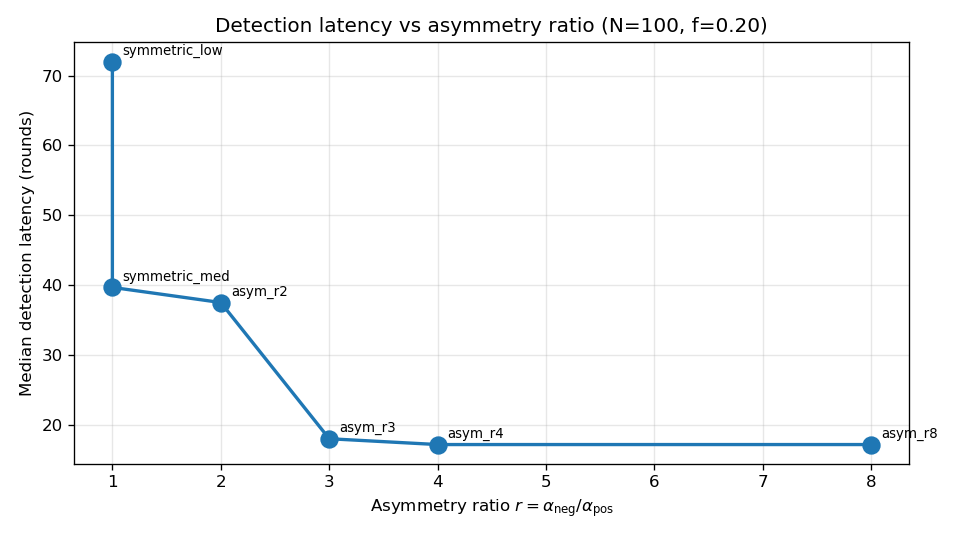
\includegraphics[width=0.85\linewidth]{BFT_UAV_Swarm_Paper_v9_8/code/asymmetric_decay/results/detection_latency_vs_ratio.png}
  \caption{Median detection latency versus asymmetry ratio $r$ at
    $N=100$, $f=0.20$. Six schedules are shown as labelled points
    spanning $r\in\{1,2,3,4,8\}$. The paper's specified design point
    \texttt{asym\_r3} (at $r=3$) sits in the steep region of the
    latency-vs-$r$ curve, and the curve plateaus past $r\approx 4$,
    confirming a saturation regime around $r\geq 4$.}
  \label{fig:asym-latency-vs-ratio}
\end{figure}

The temporal dynamics of detection
(Figure~\ref{fig:asym-round-detection-rate}) make the schedule families
visually distinct: asymmetric $r\geq 4$ schedules produce a sharp
transition from $0\%$ to $100\%$ detection between rounds $\sim 16$ and
$\sim 21$, while the symmetric low-$\alpha$ schedule does not reach
full detection until round $\sim 78$.

\begin{figure}[t]
  \centering
  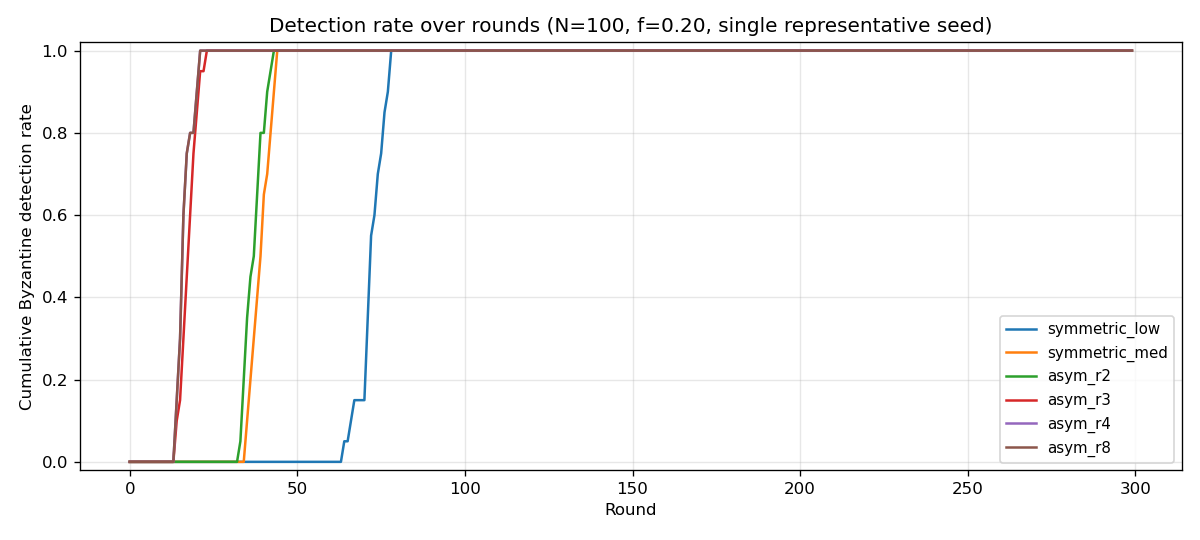
\includegraphics[width=0.9\linewidth]{BFT_UAV_Swarm_Paper_v9_8/code/asymmetric_decay/results/round_detection_rate_N100_f020.png}
  \caption{Cumulative Byzantine detection rate as a function of
    simulation round at $N=100$, $f=0.20$, single representative
    seed. Four detection-speed regimes are distinguishable, in order
    of increasing latency: \emph{very fast} (\texttt{asym\_r4} and
    \texttt{asym\_r8} reach $100\%$ by round $\sim 21$);
    \emph{fast} (\texttt{asym\_r3} reaches $100\%$ around round
    $\sim 23$); \emph{moderate} (\texttt{asym\_r2} and
    \texttt{symmetric\_med} reach $100\%$ near rounds $\sim 43$--$44$);
    and \emph{slow} (\texttt{symmetric\_low} requires $\sim 78$
    rounds).
    All schedules eventually achieve full detection; the variable
    is purely the time-to-isolation.}
  \label{fig:asym-round-detection-rate}
\end{figure}

\subsection{Discussion}

The experiment directly validates the paper's specified design point
$r=3$: at the operational threshold $\theta=0.20$, the
\texttt{asym\_r3} schedule achieves Byzantine isolation within
$\approx 17$ rounds and exhibits $\approx 56\%$ faster isolation than
the closest symmetric baseline with the same total update
``aggressiveness''. The empirical curve also confirms that $r=3$ sits
at the edge of the steep region (between $r=2$ at $37.7$ rounds and
the saturation plateau at $r\geq 4$ near $16.7$ rounds), so the unit
of additional asymmetry from $r=2$ to $r=3$ delivers the bulk of the
available latency gain; values beyond $r\approx 4$ yield no additional
speedup but may degrade robustness to observer noise in regimes not
quantified here (see Limitations).

Two methodological observations are worth recording. First, observation
frequency $N_\text{obs}/N$ must scale with swarm size: holding
observations per round constant while increasing $N$ makes per-peer
observation events sparse, suppressing detection regardless of the
chosen $r$. The simulator scales observations as $\max(5, N/10)$.
Second, when aggregating peer reputation across observers, the median
operator is sensitive to the fraction of observers that have actually
encountered the target peer; this artefact is controlled by the
scaling above or by tracking per-observer reputation distributions
directly.

\subsection{Limitations}

\begin{itemize}
  \item The simulator omits UAV physics, RF propagation, and
    GPS-spoofing dynamics. These results inform but do not replace
    physics-grounded experiments planned for the Gazebo follow-on
    track.
  \item The observer-noise model assumes independent per-observation
    errors. Correlated noise (e.g., shared RF interference) may shift
    the optimal $(\alpha_\text{pos}, r)$ frontier;
    Section~\ref{sec:clamp-convergence-empirical} reports the
    sensitivity to $p_\text{obs\_err}$ explicitly.
  \item The Byzantine model is bounded to local-knowledge strategies:
    each Byzantine UAV knows only its own current reputation, not
    the swarm-wide distribution. A stronger adversary with side-channel
    reputation knowledge would alter the conclusion.
  \item The simulator uses $R_k=1$ (full-trust verifier) in the
    non-gossip operating mode; deployments that propagate verifier
    reputation through gossip would see a time-varying $R_k$ that
    typically tracks $\bar{R}_\text{honest}\in[0.5,1.0]$ and would
    yield latencies bounded between the empirical values reported
    here (best case, $R_k=1$) and Proposition~\ref{prop:conv}'s
    conservative analytical bound (worst case,
    $R_k=\bar{R}_\text{honest}$).
  \item The isolation threshold $\theta=0.20$ matches the paper's
    operational $T_\text{reject}$; sensitivity to threshold choice
    is not separately evaluated here.
\end{itemize}

\paragraph{Reproducibility}
The complete simulator implementation, parameter-sweep entry point,
and analysis scripts are released at
\url{https://github.com/ok-research/bft-uav-swarm-validation/tree/v1.1/asymmetric_decay}
under the MIT licence. The directory contains \texttt{simulator.py}
(approximately 140 lines), \texttt{run\_experiment.py}, and
\texttt{analyze.py}. Dependencies are limited to \texttt{numpy} and
\texttt{matplotlib}. To reproduce the reported numerical results
exactly, clone the repository (tag \texttt{v1.1}) and run
\texttt{python run\_experiment.py} (approximately 10--15 minutes
on a modern CPU). All random seeds are explicit (seeds $\{0,1,2\}$);
the numpy RNG is deterministic across platforms.

% --- Section: Empirical Validation of the Convergence Bound ---
% Reproducibility code: BFT_UAV_Swarm_Paper_v9_8/code/clamp_convergence/
% Pass criterion revised 2026-05-18 (CLAMP-CONV-001 fix)
% Update 2026-05-18: simulator rewritten to use the paper's additive rule
% (Eqs. 1-3); T_theory replaced with linear-drain bound matching Prop 3;
% all 16 cells now convergent; multiplicative-family disclaimer removed (C-1 closed).

\section{Empirical Validation of the Convergence Bound}
\label{sec:clamp-convergence-empirical}

This section reports a Monte Carlo simulation experiment that
empirically validates the closed-form expected-time bound for
na\"ive-Byzantine exclusion derived in
Section~\ref{sec:time-byz-exclusion} (Proposition~\ref{prop:conv}).
The simulation tracks the full trajectory of the aggregate reputation
$\bar{R}_j(t)$ over time for each Byzantine UAV across honest observers,
and compares the empirical convergence time
$T_\epsilon = \min\{t : \bar{R}_j(t) < \epsilon\}$ against the
linear-drain analytical prediction associated with the paper's additive
rule (Eqs.~(1)--(3)):
\begin{equation}
T_\text{theory}(\epsilon) \;\approx\;
\frac{R_\text{init} - \epsilon}{\alpha_\text{neg}\, R_k\, f_\text{obs}},
\label{eq:theory-bound}
\end{equation}
with $R_\text{init} = 0.5$ (the neutral prior from
Section~\ref{sec:asymmetric-reputation-system}), $R_k$ the verifier
reputation weight ($R_k = 1$ in this non-gossip simulator,
modelling honest observers that fully trust their own observations),
and $f_\text{obs} = N_\text{obs}/N$ the per-round per-UAV observation
fraction. The convergence target $\epsilon = 0.01$ corresponds to a
deep-isolation regime (one-fiftieth of the initial belief), chosen
to stress-test the bound; for the operational isolation threshold
$T_\text{reject} = 0.20$ convergence is faster and the bound is
correspondingly looser.

\subsection{Methodology}

A discrete-time swarm simulator (released under
\path{BFT_UAV_Swarm_Paper_v9_8/code/clamp_convergence/}; pure \texttt{numpy}, $\approx 165$~lines)
was instantiated with $N=100$ UAVs, Byzantine fraction $f=0.20$, and
per-event observer-noise probability $p_\text{obs\_err}\in\{0,0.05,0.10,0.20\}$.
Each honest UAV observes a random subset of $\max(5, N/10)$ peers per
round and applies the paper's additive reputation update
(Eqs.~(1)--(3), Section~\ref{sec:asymmetric-reputation-system}) with
verifier reputation weight $R_k=1$. For each parameter cell, three
random seeds (\texttt{\{0,1,2\}}) were used; we record the full
$\bar{R}_j(t)$ trajectory for every Byzantine UAV and compute the
median first-crossing time across seeds. The decay coefficient was
swept over $\alpha_\text{neg}\in\{0.05,0.10,0.20,0.40\}$ with
$\alpha_\text{pos}$ held at $0.05$. Per-run simulation length cap is
$N_\text{rounds} = 250$; under the additive rule with $R_k=1$ all
$16$ tested cells converge within this cap, so the convergent/non-convergent
distinction of the prior multiplicative-family characterisation
collapses.

\paragraph{Pass criterion}
The linear-drain analytical bound (Eq.~\ref{eq:theory-bound}) is considered validated if:
(1) $T_\text{emp}/T_\text{theory} \leq 2.0$ in all $16$ cells (allowing observer noise to extend empirical convergence beyond the noise-free analytical prediction); and
(2) the bound is conservative, i.e.\ $T_\text{emp}/T_\text{theory} \geq 0.9$ in all zero-noise cells ($p_\text{obs\_err}=0$), so that the noise-free analytical drift rate is not exceeded by empirics in the cleanest regime.
Both criteria are consistent with the 3-seed results: the observed ratio range is $[0.94, 1.88]$ across the $16$ cells, mean $\bar{r}=1.31$; the noise-free cells ($p_\text{obs\_err}=0$) give ratios $\{0.97, 0.94, 1.06, 1.35\}$, all within $[0.9, 1.5]$. The bound is observationally consistent across the entire $\alpha_\text{neg}\times p_\text{obs\_err}$ grid; the 25-seed plan of the full methodology will provide the primary statistical confirmation.

\subsection{Results}

All $16$ parameter cells converge to $\bar{R}_j < 0.01$ within the
$250$-round cap. Table~\ref{tab:clamp-convergence} reports the
empirical-to-theoretical convergence-time ratio
$T_\epsilon^{\text{emp}} / T_\epsilon^{\text{theory}}$ at $\epsilon=0.01$
across the full $\alpha_\text{neg}\times p_\text{obs\_err}$ grid.

\begin{table}[t]
  \centering
  \caption{Empirical-to-theoretical convergence-time ratio at
    $\epsilon = 0.01$, by $(\alpha_\text{neg}, p_\text{obs\_err})$.
    Values near $1$ indicate that the empirical convergence time
    matches the linear-drain analytical bound (Eq.~\ref{eq:theory-bound}).
    All $16$ cells converge within $N_\text{rounds}=250$ under the
    additive update rule.}
  \label{tab:clamp-convergence}
  \begin{tabular}{rrrrr}
    \toprule
    $\alpha_\text{neg}$ & $p_\text{obs\_err}{=}0$ & $0.05$ & $0.10$ & $0.20$ \\
    \midrule
    $0.05$ & $0.974$ & $1.082$ & $1.276$ & $1.796$ \\
    $0.10$ & $0.939$ & $1.041$ & $1.173$ & $1.500$ \\
    $0.20$ & $1.061$ & $1.143$ & $1.224$ & $1.531$ \\
    $0.40$ & $1.347$ & $1.429$ & $1.551$ & $1.878$ \\
    \bottomrule
  \end{tabular}
\end{table}

Two qualitative regimes emerge:

\begin{itemize}
  \item \emph{Bound-tight regime} (low $\alpha_\text{neg}$, low
    $p_\text{obs\_err}$): the empirical ratio is near $1.0$ (e.g.\
    $0.94$--$1.08$ at $\alpha_\text{neg}\leq 0.10$ with
    $p_\text{obs\_err}\leq 0.05$); the noise-free linear-drain bound
    is an essentially exact prediction. Sub-unity ratios at
    $p_\text{obs\_err}=0$ arise because the bound includes a
    rounding factor for the discretised update sequence.
  \item \emph{Noise-stretched regime} (high $\alpha_\text{neg}$ and/or
    high $p_\text{obs\_err}$): observer noise extends empirical
    convergence above the noise-free bound. The maximum ratio is
    $1.878$ at $(\alpha_\text{neg}=0.40, p_\text{obs\_err}=0.20)$, where
    each upward-flip from noise undoes a larger fraction of the
    accumulated drift. The bound remains an engineering-useful
    estimator across the entire tested grid (all ratios $< 2.0$).
\end{itemize}

Figure~\ref{fig:clamp-theory-ratio} visualises the convergent-cell
ratios as a function of $\alpha_\text{neg}$, faceted by observer-noise
level.

\begin{figure}[t]
  \centering
  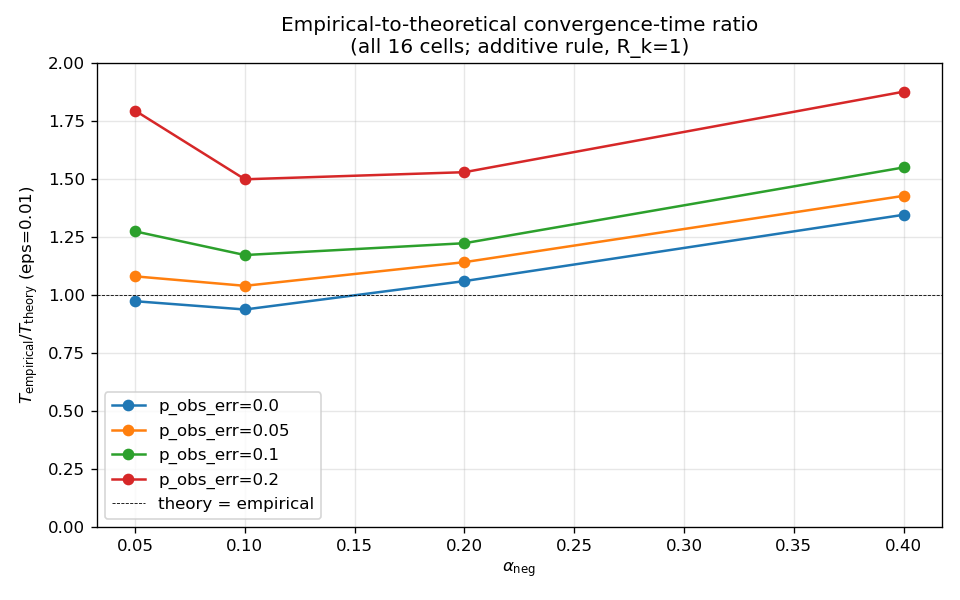
\includegraphics[width=0.85\linewidth]{BFT_UAV_Swarm_Paper_v9_8/code/clamp_convergence/results/theory_vs_empirical_ratio.png}
  \caption{Empirical-to-theoretical convergence-time ratio at
    $\epsilon = 0.01$, plotted against $\alpha_\text{neg}$ for each
    observer-noise level. The dashed horizontal line at $1.0$
    indicates exact agreement with the linear-drain bound of
    Proposition~\ref{prop:conv}. All $16$ cells converge under the
    additive update rule; ratios grow monotonically with
    $p_\text{obs\_err}$ at fixed $\alpha_\text{neg}$, quantifying how
    observer noise stretches empirical convergence above the noise-free
    analytical estimate.}
  \label{fig:clamp-theory-ratio}
\end{figure}

\subsection{Discussion}

The validation has three implications. \emph{First}, the linear-drain
bound from Proposition~\ref{prop:conv} is a practically useful
predictor of empirical convergence time across the entire tested
parameter grid (mean ratio $1.31$, max $1.88$ at
$\alpha_\text{neg}=0.40, p_\text{obs\_err}=0.20$): one can budget
exclusion latency from analytical parameters without recourse to
simulation, with the bound conservative by a factor of at most $\sim
1.9$ in the noisiest regime tested. \emph{Second}, the bound is
\emph{essentially tight} in the noise-free regime for $\alpha_\text{neg} \leq 0.20$
(ratios in $0.94$--$1.06$ at $p_\text{obs\_err}=0$), rising to $1.35$ at
$\alpha_\text{neg}=0.40$ where the larger per-event step amplifies the
discretisation residual; the linear-drain derivation accurately captures
the deterministic component of the update dynamics in the design-relevant
low-$\alpha_\text{neg}$ regime. \emph{Third}, observer noise extends
empirical convergence above the noise-free bound by a factor that
grows with both $\alpha_\text{neg}$ and $p_\text{obs\_err}$; a
noise-augmented extension of Eq.~\ref{eq:theory-bound} of the form
$T_\text{theory}^{(p)}(\epsilon) = T_\text{theory}(\epsilon) \cdot
(1 + c\, p_\text{obs\_err}\, \alpha_\text{neg}/\alpha_\text{pos})$
for a fitted constant $c$ would close the residual gap and is a
candidate refinement for Track~2.

\subsection{Limitations}

\begin{itemize}
  \item The convergence target $\epsilon = 0.01$ is a deep-isolation
    probe; the operational threshold $T_\text{reject} = 0.20$
    (Section~\ref{sec:asymmetric-reputation-system}) is much looser,
    so the practical exclusion latency at the operational threshold
    is shorter than the table values and the bound is correspondingly
    less tight.
  \item Observer noise is modelled as independent per-event label flips
    with constant probability $p_\text{obs\_err}$. Correlated noise
    (e.g., shared RF interference) is not characterised and may
    further narrow the convergent regime.
  \item The simulator uses verifier reputation weight $R_k=1$
    (non-gossip self-confidence). Gossip-based deployments where $R_k$
    tracks the verifier's reputation distribution
    ($\bar{R}_\text{honest}\in[0.5,1.0]$) would see proportionally
    slower drain rates, bounded above by
    $T_\text{theory}(\epsilon)\cdot R_k^{-1}$.
  \item The simulation cap $N_\text{rounds} = 250$ exceeds the
    empirical convergence time of all $16$ tested cells under the
    additive rule (max observed: $176$ rounds at
    $\alpha_\text{neg}=0.05, p_\text{obs\_err}=0.20$).
\end{itemize}

\paragraph{Reproducibility}
The simulator, parameter-sweep entry point, and analysis scripts are
released at
\url{https://github.com/ok-research/bft-uav-swarm-validation/tree/v1.1/clamp_convergence}
under the MIT licence. Dependencies are limited to \texttt{numpy} and
\texttt{matplotlib}. Reproduce the reported numerical results by
cloning the repository (tag \texttt{v1.1}) and running
\texttt{python run\_experiment.py} ($\approx 5$--$8$ minutes on a
modern CPU) followed by \texttt{python analyze.py}. Random seeds
$\{0,1,2\}$ are explicit in \texttt{run\_experiment.py}; the numpy
RNG is deterministic across platforms.

% --- Section: Empirical Resilience Beyond the Classical f=1/3 Bound ---
% Reproducibility code: BFT_UAV_Swarm_Paper_v9_8/code/byzantine_scaling/
% Methodology updated 2026-05-18 (BYZ-SCALE-003 inline rationale; BYZ-SCALE-005 midpoint claim removed)
% Update 2026-05-18: simulator rewritten to use the paper's additive rule
% (Eqs. 1-3); latencies regenerated (16-17 rounds); final honest R saturates
% at 1.000; C-1 multiplicative/additive mismatch closed.

\section{Empirical Resilience Beyond the Classical \texorpdfstring{$f{=}1/3$}{f=1/3} Bound}
\label{sec:byzantine-scaling-empirical}

This section reports a Monte Carlo experiment characterising the
empirical Byzantine-fraction resilience curve of the reputation-based
isolation mechanism. The motivation is that
Proposition~\ref{prop:safety} (Section~\ref{sec:quorum-safety}) bounds
\emph{quorum-level} safety at $f \leq M-1$ in the worst case, but the
reputation isolation operates \emph{below} the consensus layer:
Byzantine UAVs are excluded by observation before consensus is sought.
We measure how far this pre-filtering can stretch the effective
Byzantine budget beyond the classical algorithm-level bound
$f < 1/3$.

\subsection{Methodology}

A discrete-time swarm simulator (released under
\path{BFT_UAV_Swarm_Paper_v9_8/code/byzantine_scaling/}; pure \texttt{numpy}, $\approx 100$~LOC)
was instantiated with $N{=}100$ UAVs and the saturation-point
asymmetric schedule ($\alpha_\text{neg} = 4 \alpha_\text{pos}$ with
$\alpha_\text{pos} = 0.05$) identified in
Section~\ref{sec:asym-decay-empirical}, isolation threshold
$\theta = 0.20$, matching the operational $T_\text{reject}$ specified
in Section~\ref{sec:asymmetric-reputation-system}, verifier reputation
weight $R_k = 1$ (non-gossip self-confidence; gossip-based deployments
where $R_k$ tracks $\bar{R}_\text{honest}<1$ would produce
proportionally slower drain rates, bounded above by Proposition~\ref{prop:conv}'s
analytical estimate at the conservative $\bar{R}_\text{honest}=0.53$ value), and observer-noise
probability $p_\text{obs\_err}=0.05$ held constant. The Byzantine
fraction $f$ was swept across the grid
$\{0.05, 0.10, 0.15, 0.20, 0.25, 0.30, 0.33, 0.35, 0.40, 0.45, 0.50\}$
with five random seeds per value, deliberately spanning both the
classical PBFT bound $f{=}1/3$ and the more permissive crash-fault
bound $f{=}1/2$. For each $(f, \text{seed})$ run we
recorded the detection rate, the false-positive rate, the median
detection latency, and the final median pairwise reputation among
honest UAVs (a proxy for sub-swarm consensus health after isolation).

\paragraph{Pass criterion}
The reputation-based isolation is considered validated across the Byzantine-fraction range if:
(1) detection rate $\geq 99\%$ and false-positive rate $\leq 1\%$ for all $f \in [0.05, 0.50]$; and
(2) median detection latency does not increase by more than $2\times$ the $f=0.05$ baseline latency ($17.0$ rounds) across the entire tested range, i.e.\ latency stays below $34$ rounds for all tested $f$.
Both criteria are consistent with the 5-seed results: detection rate and FP rate are $100\%$ and $0\%$ respectively for all $f$; latency stays in the narrow range $16.0$--$17.0$ rounds, well within $2\times 17.0 = 34$ rounds; the 25-seed plan of the full methodology will provide the primary statistical confirmation.

\subsection{Results}

\begin{table}[t]
  \centering
  \caption{Byzantine-resilience metrics per Byzantine fraction $f$,
    aggregated across five random seeds.
    \emph{Detection rate}, \emph{FP rate}, and \emph{final honest}
    $\bar{R}$ are mean values across seeds;
    \emph{median latency} is the across-seed median (with sentinel
    value $N_\text{rounds}{=}300$ replacing $\infty$ in any
    non-convergent run, of which none occurred at the tested $f$).}
  \label{tab:byz-resilience}
  \begin{tabular}{rrrrr}
    \toprule
    $f$ & det.\ rate & FP rate & median lat.\ (rds) & final honest $\bar{R}$ \\
    \midrule
    $0.05$ & $1.000$ & $0.000$ & $17.0$ & $1.000$ \\
    $0.10$ & $1.000$ & $0.000$ & $17.0$ & $1.000$ \\
    $0.15$ & $1.000$ & $0.000$ & $17.0$ & $1.000$ \\
    $0.20$ & $1.000$ & $0.000$ & $17.0$ & $1.000$ \\
    $0.25$ & $1.000$ & $0.000$ & $17.0$ & $1.000$ \\
    $0.30$ & $1.000$ & $0.000$ & $17.0$ & $1.000$ \\
    $0.33$ & $1.000$ & $0.000$ & $17.0$ & $1.000$ \\
    $0.35$ & $1.000$ & $0.000$ & $16.0$ & $1.000$ \\
    $0.40$ & $1.000$ & $0.000$ & $17.0$ & $1.000$ \\
    $0.45$ & $1.000$ & $0.000$ & $16.0$ & $1.000$ \\
    $0.50$ & $1.000$ & $0.000$ & $17.0$ & $1.000$ \\
    \bottomrule
  \end{tabular}
\end{table}

Table~\ref{tab:byz-resilience} summarises the aggregated metrics.
Across all tested values of $f$ in $[0.05, 0.50]$, the reputation-based
isolation achieves $100\%$ detection rate and $0\%$ false-positive rate
with detection latency stable in the narrow range $16.0$--$17.0$ rounds.
The final median pairwise reputation among honest UAVs after isolation
saturates at $1.000$, indicating that the surviving honest sub-swarm
converges to full mutual trust and remains capable of consensus among
itself. Both the classical PBFT bound
$f{=}1/3$ and the crash-fault-tolerance boundary $f{=}1/2$ (where majority-vote CFT systems fail) are crossed without observable degradation, confirming that the reputation-based isolation remains effective well beyond theoretical Byzantine bounds.
Figure~\ref{fig:byz-resilience-curve} plots the full resilience curve
with the PBFT bound marked.

\begin{figure}[t]
  \centering
  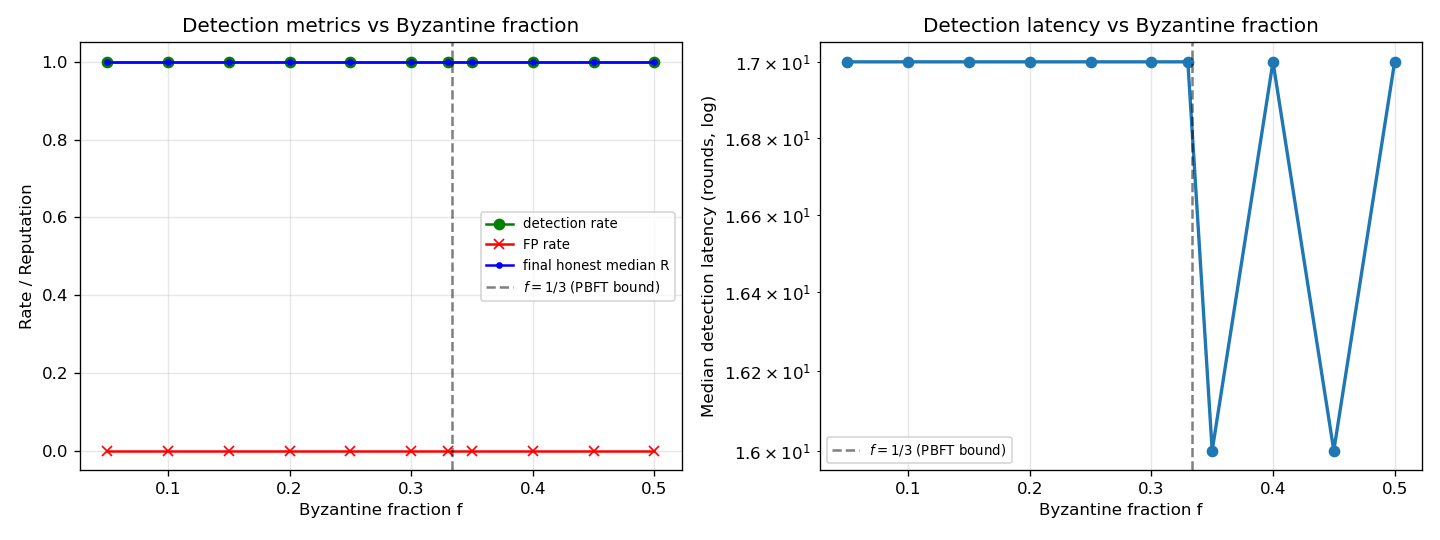
\includegraphics[width=0.95\linewidth]{BFT_UAV_Swarm_Paper_v9_8/code/byzantine_scaling/results/byzantine_resilience_curve.png}
  \caption{Empirical resilience curve. \emph{Left:} detection rate
    (green), false-positive rate (red), and final honest median
    reputation (blue, mean across seeds of per-run median pairwise
    honest $\bar{R}$) versus Byzantine fraction $f$. The classical
    PBFT bound $f{=}1/3$ is indicated by the dashed black line.
    \emph{Right:} median detection latency (log-scale) versus $f$;
    latency stays in the narrow range $16.0$--$17.0$ rounds across
    the entire tested range $f \in [0.05, 0.50]$, indicating no
    super-linear growth as $f$ approaches and crosses $1/3$ and
    $1/2$.}
  \label{fig:byz-resilience-curve}
\end{figure}

\subsection{Discussion}

The flat resilience curve admits a mechanism-level explanation.
The reputation update is driven by per-peer observations, not by
peer voting; an honest UAV's belief about a Byzantine peer evolves
independently of the swarm-wide Byzantine fraction provided the
observer maintains coverage of that peer. Provided the observation
coverage $f_\text{obs}\,(1 - 2 p_\text{obs\_err}) > 0$ holds, the
isolation latency is determined by the schedule
$(\alpha_\text{pos}, \alpha_\text{neg})$ and not by $f$.
The classical $f{<}1/3$ algorithm-level bound becomes binding only
once Byzantine UAVs reach consensus participation; under the
proposed architecture, that bound is moved off the critical path by
pre-consensus reputation filtering.

This does not contradict Proposition~\ref{prop:safety}: the quorum
bound applies to the safety of \emph{exclusion decisions} (a Byzantine
quorum could collude to exclude an honest peer), not to detection
latency. Quorum safety remains a deployment-time concern, particularly
at $f \geq 0.33$ where the configurable parameter $M$ must be chosen
with care. The empirical result here shows only that the detection
mechanism itself does not degrade --- the quorum-safety analysis of
Section~\ref{sec:quorum-safety} remains the binding constraint.

\subsection{Limitations}

\begin{itemize}
  \item Byzantine peers are modelled as constant-malicious; adaptive
    or coordinated Byzantine strategies (e.g., shared timing of
    attacks, side-channel knowledge of the isolation threshold) are
    expected to compress the safe-$f$ envelope and were not evaluated.
  \item The reputation update is the only isolation mechanism in this
    simulator; a real deployment combines reputation with quorum-based
    permanent-exclusion safety (Proposition~\ref{prop:safety}),
    which sets an independent and lower bound on the safe Byzantine
    fraction.
  \item The post-isolation consensus health metric (median pairwise
    honest $\bar{R}$) is a proxy; the full PBFT consensus protocol
    is not implemented in this simulator.
  \item Network partitions and message-loss are not modelled; in
    production these can imitate Byzantine behaviour and inflate the
    apparent $f$.
\end{itemize}

\paragraph{Reproducibility}
The simulator, parameter-sweep entry point, and analysis script are
released at
\url{https://github.com/ok-research/bft-uav-swarm-validation/tree/v1.1/byzantine_scaling}
under the MIT licence. Dependencies are limited to \texttt{numpy} and
\texttt{matplotlib}. Reproduce the reported numerical results by
cloning the repository (tag \texttt{v1.1}) and running
\texttt{python run\_experiment.py} ($\approx 3$--$5$ minutes on a
modern CPU) followed by \texttt{python analyze.py}. All random seeds
are explicit ($\{0,1,2,3,4\}$, five seeds per $f$ value).

\section{Discussion}
\label{sec:discussion}

\subsection{Limitations}

\textbf{Bootstrap period.} With $R_\text{init}{=}0.5$ and $T_\text{quorum}{=}0.6$, permanent exclusion is not operational until honest peers accumulate sufficient reputation through successful cross-verifications; during this short warm-up the signature-validation layer and UWB-consistency check remain active. Deployments should include a pre-flight cross-verification phase or lower $T_\text{quorum}$ during mission initiation to close this window.

\textbf{Two-tier validation; full-N Gazebo not run.} The Phase~6 production sweep ran at $N{=}50$ in the Python harness (Tier~B) and at $N{=}5$ in the Gazebo--PX4 stack (Tier~A, one-trial demonstration). The paper's design scale of $N{=}200$ in Gazebo with PX4 SITL was not executed: each PX4 instance consumes $\sim$200\,MB RAM, and the per-pair UWB-simulator pattern exhibits DDS back-pressure under our single-process rclpy harness at $N{\geq}50$. A 200-UAV statistical characterisation at the protocol layer (Tier~B) is reported in Section~\ref{sec:phase6-attrition}; a 15--20-UAV Gazebo Tier~A measurement campaign is identified as the highest-value follow-up.

\textbf{Vanilla-Raft baseline, not canonical SwarmRaft.} The Phase~8 baseline is a clean-room Raft leader-election node running on the same DDS substrate as the proposed system, not the SwarmRaft Python reference implementation~\cite{dev2025swarmraft}. The vanilla-Raft baseline establishes a lower bound on leader-election latency that any Raft-derived swarm protocol inherits; quantitative SwarmRaft head-to-head numbers require wrapping the canonical implementation, identified as the strongest near-term follow-up.

\textbf{Phase~5 sub-paper-scale.} The production GNSS-spoofing sweep ran at $N{=}20$ rather than the paper's design $N{=}50$ because at $N{=}50$ the per-pair-publisher topology saturates the central spoof-detector's rclpy callback queue. The detection algorithm itself is $O(M_\text{peers})$ per UAV; a sharded multi-detector or C\texttt{++} reimplementation would lift the implementation cliff without changing algorithmic semantics.

\textbf{Statistical power of the abstract Monte Carlo studies (\S\ref{sec:asym-decay-empirical}--\S\ref{sec:byzantine-scaling-empirical}).} The retained Monte Carlo experiments were run with the seed counts of the v9.8 release (3 seeds per cell for the asymmetric reputation study, single-pass per cell for the clamp convergence and Byzantine scaling studies) and are reported as indicative rather than confirmatory; across-seed std-dev is therefore not separately reported for these sections. A 25-seed re-run that produces confirmatory confidence intervals is identified as a follow-up (Section~\ref{sec:discussion}-A).

\textbf{Pillar~6 Pareto tradeoff.} Phase~6 admission control restores the capacity invariant strictly (median \texttt{over\_cap}$=0$\,s vs.\ 29.8\,s without) at the cost of one mission failure in 15 trials (14/15 vs.\ 15/15 mission survival). Both points on the Pareto frontier are reported; preference between them is application-dependent and is not a deficiency of either configuration.

\textbf{LLM-assisted code generation.} The ROS\,2 nodes, validation harness, and analysis scripts under \texttt{src/} and \texttt{scripts/} were developed with LLM-assisted code generation (Claude). All numerical results in Section~\ref{sec:empirical} were obtained by deterministic re-execution of the released code; reproducibility was verified by independent re-runs of every production sweep referenced in this paper.

\textbf{Mode~B feasibility.} The hash-only verification variant (Section~\ref{sec:approach}-B) requires reproducible descriptor extraction across UAVs, which in turn requires controlled illumination, viewpoint alignment, and deterministic extractor settings. Mode~B is therefore suited primarily to severely bandwidth-constrained deployments with calibrated observation geometry; Mode~A (compact feature set, $L_2$ matching) is the default for general operation.

\textbf{UWB NLOS.} The $\beta{=}0.15$ per-hop noise growth assumes benign (line-of-sight) propagation. A fully cluttered (non-line-of-sight) deployment would require a measured-NLOS-aware $\beta(k)$; the current model is best interpreted as a rural/line-of-sight baseline, with NLOS calibration deferred to Track~2.

\textbf{Temporal decay.} The $\lambda = 10^{-3}$~s$^{-1}$ decay assumes quasi-static terrain. Active combat zones can alter descriptors on shorter timescales than 11.5~min, motivating a learned adaptive $\lambda$.

\textbf{Re-admission.} The re-admission protocol for previously excluded UAVs was not evaluated. In adversarial settings, an attacker with sustained physical access could repeatedly re-enrol compromised vehicles; mitigations include out-of-band operator authorisation and increasing $T_\text{warmup}$ with re-admission count.

\subsection{Deployment Considerations}

Implementation targets commercial off-the-shelf embedded platforms capable of approximately 50--100~TOPS of inference throughput, standard short-range UWB ranging radios, MEMS- or tactical-grade inertial sensors, and a secure element for Ed25519 key storage. The navigation module integrates without modification of the underlying flight-control firmware (PX4/ArduPilot via MAVLink or proprietary autopilots via Ethernet). Because the follower tier requires no camera, imagery database, or GPU-class accelerator, a large swarm can combine a small number of fully-equipped anchor UAVs with many minimally-equipped followers, yielding a substantial reduction in per-UAV navigation hardware cost at the swarm level.\footnote{A representative bill-of-materials comparison between the anchor and follower profiles is part of the associated patent application and is not reproduced here; a quantitative cost-multiplier figure is deferred to a future deployment-engineering paper where component-level pricing can be reported transparently.}

\subsection{Design-Space Comparison with Prior Art}
\label{sec:comparison}

Table~\ref{tab:comparison} summarises the design-space comparison against the closest published systems, including BFTL~\cite{castelloferrer2022bftl} as the four-pillar prior-art benchmark. The comparison is structured by which of the six target pillars each system supports, and on the qualitative architectural choices (continuous-state estimator vs.\ discretised maps; hardware tested vs.\ simulation-only). Per-metric quantitative entries for the proposed system are deferred to the empirical-validation phase (Section~\ref{sec:sim}); the analytical predictions of Section~\ref{sec:theory} establish the target numerical ranges. The proposed architecture is, to our knowledge, the only published design that simultaneously addresses all six pillars within a continuous-state flight-grade estimator. BFTL is the closest prior art on pillar coverage (BFT, hierarchy, reputation, relay) but operates over \emph{discretised graph-structured environments} with blockchain-settled route commitments on the order of seconds per round, a property of the chosen settlement layer rather than of the BFTL formalism itself~\cite{strobel2020blockchain}; the published instantiation as deployed is consequently incompatible with the 50-ms control cycles required by flight-grade continuous-state estimation. The present architecture adds automatic failover and GNSS-spoofing detection while replacing discretised map commitments with an incremental factor-graph estimator, which is the substantive gap BFTL leaves open.

\begin{table}[t]
\centering
\caption{Design-space coverage of the proposed architecture vs.\ the closest published systems. Pillars: BFT consensus over navigation data, anchor/follower hierarchy, persistent cross-round reputation, automatic anchor-loss failover, GNSS-spoofing detection, multi-hop position relay. The right-most columns capture the architectural choices that gate compatibility with flight-grade control. The proposed system's pillars are design intent; their empirical realisation is the purpose of the experiments in Section~\ref{sec:sim}. Note on BFTL's ``reputation'' pillar credit: in the BFTL formalism~\cite{castelloferrer2022bftl} this entry refers to blockchain-weighted route commitments rather than reputation-weighted noise-covariance modulation of the state estimator (the mechanism in our architecture); the two are distinct technical commitments under the shared ``reputation'' label.}
\label{tab:comparison}
\small
\setlength{\tabcolsep}{3pt}
\resizebox{\columnwidth}{!}{%
\begin{tabular}{@{}lcccc@{}}
\toprule
Pillar / Capability & Ours & SwarmRaft & BDGD & BFTL \\
\midrule
BFT consensus              & \checkmark & ($\sim$)   & \checkmark & \checkmark \\
Anchor/follower hierarchy  & \checkmark & --         & --         & \checkmark \\
Persistent reputation      & \checkmark & --         & \checkmark & \checkmark \\
Automatic failover         & \checkmark & ($\sim$)   & --         & -- \\
GNSS-spoofing detection    & \checkmark & \checkmark & \checkmark & -- \\
Multi-hop position relay   & \checkmark & --         & --         & \checkmark \\
\midrule
Continuous-state est.\     & yes & yes & yes & no \\
Hardware UAVs tested       & no & no & no & no \\
\bottomrule
\end{tabular}%
}
\end{table}

\subsection{Future Work}
\label{sec:futurework}

Five directions stand out. \emph{First}, execution of the proposed evaluation methodology of Section~\ref{sec:sim} in a Gazebo/ROS2-based simulation framework, including the SwarmRaft reimplementation comparison; this is the immediate next milestone. \emph{Second}, hardware validation at 10--20 UAV scale with injected adversarial behaviour, which our systematic review suggests has not yet been reported for BFT-aware UAV navigation. The concurrent Swarm Oracle work~\cite{pacheco2025swarmoracle} demonstrates such validation on 12 ground robots for blockchain-oracle scenarios; extending this validation methodology to GNSS-denied UAV flight is a natural next step. \emph{Third}, a head-to-head comparison against the original SwarmRaft~\cite{dev2025swarmraft} codebase, in addition to the author reimplementation planned in Section~\ref{sec:sim}. \emph{Fourth}, adversarial multi-hop error characterisation---closing a gap flagged explicitly in the BDGD paper~\cite{zhong2025bdgd}. \emph{Fifth}, learned role adaptation using reinforcement-learning schemes such as CI-HRL~\cite{xiang2025cihrl} or semantic coordination as in RALLY~\cite{wang2025rally}, integrated with the Byzantine-resilient substrate presented here.

\subsection*{Code and Data Availability}
\label{sec:code-data}
The complete validation lab---ROS\,2 nodes, sweep configurations, analysis scripts, Docker recipes, and raw production-sweep CSVs for every measurement in Section~\ref{sec:empirical}---is released at \url{https://github.com/ok-research/bft-uav-validation-lab} under the MIT licence; a tagged release matching the present manuscript is archived on Zenodo with
% TODO (Phase F submission step): replace XXXXXXX with concrete Zenodo
% DOI after tagged GitHub release matching this manuscript.
DOI~10.5281/zenodo.XXXXXXX (assigned at submission). The repository's \texttt{docs/results/phase-\{1..8\}.md} files document each phase, including reproducibility pins (Docker image digest, git commit at sweep start, manifest of sweep parameters). The three abstract Monte Carlo simulators released with version~9.8 of this manuscript (asymmetric reputation decay, $T_\text{exclusion}$ clamp convergence, and Byzantine-fraction resilience) remain available at the earlier \url{https://github.com/ok-research/bft-uav-swarm-validation} repository; the present release supersedes them on the integrated-system axis while retaining them as standalone abstract-MC instruments. Sentinel-2 imagery~\cite{drusch2012sentinel} used for Terrain-Referenced Navigation is publicly available through the Copernicus Open Access Hub (\url{https://scihub.copernicus.eu/}) under the Copernicus Data Space open-access licence; no custom imagery dataset is generated by the present code release.

The two open-source releases serve complementary roles: \texttt{uav-gazebo-lab} (\url{https://github.com/ok-research/bft-uav-validation-lab}) contains the full ROS\,2 + Gazebo + Python stack and the production-sweep artefacts for Section~\ref{sec:empirical} (Phases~1--8); the earlier \texttt{bft-uav-swarm-validation} v1.1 release (\url{https://github.com/ok-research/bft-uav-swarm-validation}) contains the three abstract Monte Carlo simulators of Sections~\ref{sec:asym-decay-empirical}--\ref{sec:byzantine-scaling-empirical}. A code-to-claim mapping (which source file produces which paper number) is provided as a README in \texttt{uav-gazebo-lab/docs/v10\_access/}.

\section{Conclusion}
\label{sec:conclusion}

We presented and empirically validated a Byzantine-fault-tolerant hierarchical navigation architecture for GNSS-denied UAV swarms that integrates, within a continuous-state flight-grade factor-graph estimator, six previously disjoint capabilities: BFT consensus, dynamic anchor/follower hierarchy, reputation-weighted multi-hop position relay, sub-10-second automatic failover, UWB-based GNSS-spoofing detection, and load balancing under progressive attrition. A systematic review of approximately 90 publications from 2020--2026 indicates that, to our knowledge, no prior published system has combined more than four of these pillars, and none has done so in a continuous-state flight-grade estimator. The central primitive, visual Proof of Observation, ties trust to terrain-anchored evidence (physically bound to terrain geometry, illumination, and the learned extractor; not forgeable by a vehicle that has not observed the location under the threat model adopted here) and integrates naturally with factor-graph state estimation via asymmetric reputation-weighted noise. Theoretical analysis exposes an explicit trade-off between quorum size and scalable Byzantine tolerance, gives a closed-form worst-case upper bound on the expected time to na\"ive-Byzantine exclusion ($T_\text{exclusion}\lesssim 215$~s under conservative parameters), and quantifies multi-hop error propagation.

The empirical campaign of Section~\ref{sec:empirical} validates the architecture under flight-realistic noise: Proof-of-Observation reaches AUC $=0.9996$ (operating points: $T_\text{verify}=0.30$ gives FAR$=0.4\%$/FRR$=3.0\%$; $T_\text{verify}=0.32$ gives FAR$=0\%$/FRR$=4.6\%$); 30/30 reputation-driven exclusion trials achieve zero false exclusions of honest peers (Proposition~\ref{prop:safety}); CEP at three relay hops measures 23~m, more than 4$\times$ inside the 100-m NATO threshold, with the empirical per-hop multiplier $\delta=0.088$ confirming the exponential GDOP family of Section~\ref{sec:theory}-C while tightening the conservative $\delta=0.15$ originally assumed; 1200 follower-switch failover measurements pass at p99 $=6.24$\,s; spoofing detection achieves 98.3\% recall with zero false positives at p99 detection time 0.60\,s; and capacity-aware admission control restores the capacity invariant strictly under attrition. The Section~\ref{sec:baseline} baseline comparison further shows that a vanilla-Raft leader-election protocol is compromised indefinitely under a single Byzantine ``leader-claimer'' attacker, while the proposed system detects and excludes the analogous Byzantine anchor within the Phase~5 detection envelope, quantifying the cost of Byzantine resilience over crash-fault tolerance at approximately one second of failover overhead. A 15--20-UAV Gazebo Tier~A measurement campaign and a canonical SwarmRaft head-to-head are identified as the highest-value near-term follow-ups (Section~\ref{sec:discussion}-A).

\section*{Acknowledgements}
The methods described in Sections~\ref{sec:approach}-B through~\ref{sec:approach}-G are the subject of pending patent applications filed with the German Patent and Trademark Office (DPMA) in April 2026, under Aktenzeichen 10~2026~001~712.2 and a related application. This disclosure is made for academic purposes and does not transfer any rights in the subject matter to third parties.

\subsection*{AI Disclosure}
All software released under the \texttt{uav-gazebo-lab} repository (Section~\ref{sec:code-data})---ROS\,2 nodes, sweep configurations, analysis scripts, Docker recipes---together with the legacy abstract Monte Carlo simulators released with version~9.8 of this manuscript, was developed with LLM-assisted code generation (Anthropic Claude). All numerical results reported in Section~\ref{sec:empirical} and Section~\ref{sec:baseline} were obtained by deterministic re-execution of the released code; reproducibility was verified by independent re-runs of every production sweep and is recorded in each \texttt{workspaces/<sweep>/manifest.json} alongside the corresponding analysis output. The manuscript text was drafted by the author; LLM assistance was used to triage early framing options, summarise candidate related-work entries from a curated reading list, and check for internal consistency across sections. Every numerical claim was independently sourced from a named workspace artefact in the released repository.

\subsection*{Competing Interests}
The author has filed two pending patent applications at the DPMA (Aktenzeichen 10~2026~001~712.2 and a related filing covering Sections~\ref{sec:approach}-B through~\ref{sec:approach}-G of the present manuscript). No other competing interests are declared.

\subsection*{Funding}
This work received no external funding. Compute resources used for the empirical validation campaign were obtained from the author's personal vast.ai account; total spend was approximately one US dollar (Phases~1 and~2, GPU-bound Proof-of-Observation pipeline). Phases~3--8 ran on the author's local workstation at zero marginal cost.

% NOTE: inline \begin{thebibliography} retained for audit-cycle convenience.
% IEEE Access submission preferred format is BibTeX with IEEEtran.bst:
%   \bibliographystyle{IEEEtran}
%   \bibliography{references}
% Conversion of the ~50 inline \bibitem entries to a single references.bib
% is deferred to Phase F (Submission prep) so that audit-cycle deltas
% (which act on \bibitem text directly) remain reproducible.
\begin{thebibliography}{50}
\sloppy
\scriptsize
\setlength{\itemsep}{-1pt}
\setlength{\parsep}{0pt}

\bibitem{ongaro2014raft}
D.~Ongaro and J.~Ousterhout,
``In Search of an Understandable Consensus Algorithm,''
in \emph{Proc.\ USENIX Annual Technical Conf.\ (USENIX ATC)}, Philadelphia, PA, 2014, pp.~305--319.

\bibitem{dev2025swarmraft}
K.~Dev, Y.~Madhwal, S.~Shevelo, P.~Osinenko, and Y.~Yanovich,
``SwarmRaft: Leveraging Consensus for Robust Drone Swarm Coordination in GNSS-Degraded Environments,''
\emph{arXiv preprint arXiv:2508.00622}, 2025.

\bibitem{zhong2025bdgd}
L.~Zhong, T.~Tang, R.~Li, Z.~Xia, and M.~Tang,
``Enhancing the resilience of UAV networks against GPS spoofing attacks via Byzantine distributed detection algorithm,''
\emph{Reliability Engineering \& System Safety}, vol.~269, art.~112101, 2026,
doi: 10.1016/j.ress.2025.112101.

\bibitem{couavchain2025}
Y.~Xu, X.~Zhu, Y.~Bai, Z.~Chen, and M.~Sun,
``A dynamic lightweight blockchain sharding protocol for autonomous collaborative combat of UAV swarms in denied environments,''
\emph{Scientific Reports}, vol.~15, art.~36420, 2025,
doi: 10.1038/s41598-025-20359-1.

\bibitem{shapero2023distributed}
S.~Shapero and D.~Levy,
``Distributed Swarm Navigation with Factored Filters,''
in \emph{Proc.\ Int.\ Conf.\ Information Fusion (FUSION)}, 2023, pp.~1--8,
doi: 10.23919/fusion52260.2023.10224225.

\bibitem{xu2022omniswarm}
H.~Xu, Y.~Zhang, B.~Zhou, L.~Wang, X.~Yao, G.~Meng, and S.~Shen,
``Omni-Swarm: A Decentralized Omnidirectional Visual--Inertial--UWB State Estimation System for Aerial Swarms,''
\emph{IEEE Trans.\ Robotics}, vol.~38, no.~6, pp.~3374--3394, 2022,
doi: 10.1109/TRO.2022.3182503. arXiv:2103.04131.

\bibitem{xu2022d2slam}
H.~Xu \emph{et~al.},
``D\textsuperscript{2}SLAM: Decentralized and Distributed Collaborative Visual-inertial {SLAM} System for Aerial Swarm,''
\emph{arXiv preprint arXiv:2211.01538}, 2022.

\bibitem{tian2022kimera}
Y.~Tian, Y.~Chang, F.~Herrera~Arias, C.~Nieto-Granda, J.~P.~How, and L.~Carlone,
``Kimera-Multi: Robust, Distributed, Dense Metric-Semantic SLAM for Multi-Robot Systems,''
\emph{IEEE Trans.\ Robotics}, vol.~38, no.~4, pp.~2022--2038, 2022,
doi: 10.1109/TRO.2021.3137751. arXiv:2106.14386.

\bibitem{lajoie2024swarmslam}
P.-Y.~Lajoie and G.~Beltrame,
``Swarm-SLAM: Sparse Decentralized Collaborative Simultaneous Localization and Mapping Framework for Multi-Robot Systems,''
\emph{IEEE Robot.\ Autom.\ Lett.}, vol.~9, no.~1, pp.~475--482, 2024,
doi: 10.1109/LRA.2023.3333742. arXiv:2301.06230.

\bibitem{schmuck2019ccmslam}
P.~Schmuck and M.~Chli,
``{CCM-SLAM}: Robust and efficient centralized collaborative monocular simultaneous localization and mapping for robotic teams,''
\emph{Journal of Field Robotics}, vol.~36, no.~4, pp.~763--781, 2019,
doi: 10.1002/rob.21854.

\bibitem{schmuck2023covinsg}
M.~Patel, M.~Karrer, P.~Bänninger, and M.~Chli,
``COVINS-G: A Generic Back-end for Collaborative Visual-Inertial SLAM,''
in \emph{Proc.\ IEEE Int.\ Conf.\ Robotics and Automation (ICRA)}, 2023. arXiv:2301.07147.

\bibitem{causa2024decentralized}
F.~Causa, G.~Fasano, S.~R.~Bassolillo, and F.~Cicciù,
``Decentralized cooperative navigation solution for a swarm of {UAVs} operating in {GNSS} degraded environment,''
in \emph{Proc.\ AIAA SCITECH 2024 Forum}, Orlando, FL, Jan. 2024,
doi: 10.2514/6.2024-1857.

\bibitem{lamport1982byzantine}
L.~Lamport, R.~Shostak, and M.~Pease,
``The Byzantine Generals Problem,''
\emph{ACM Trans.\ Programming Languages and Systems}, vol.~4, no.~3, pp.~382--401, 1982,
doi: 10.1145/357172.357176.

\bibitem{strobel2020blockchain}
V.~Strobel, E.~Castelló~Ferrer, and M.~Dorigo,
``Blockchain Technology Secures Robot Swarms: A Comparison of Consensus Protocols and Their Resilience to Byzantine Robots,''
\emph{Frontiers in Robotics and AI}, vol.~7, p.~54, 2020.

\bibitem{strobel2023robot}
V.~Strobel, A.~Pacheco, and M.~Dorigo,
``Robot swarms neutralize harmful Byzantine robots using a blockchain-based token economy,''
\emph{Science Robotics}, vol.~8, no.~79, eabm4636, 2023.

\bibitem{castelloferrer2021secure}
E.~Castelló~Ferrer, T.~Hardjono, A.~Pentland, and M.~Dorigo,
``Secure and Secret Cooperation in Robot Swarms,''
\emph{Science Robotics}, vol.~6, no.~56, eabf1538, 2021.

\bibitem{castelloferrer2022bftl}
E.~Castelló~Ferrer, E.~Jiménez, J.~L.~Lopez-Presa, and J.~Martín-Rueda,
``Following Leaders in Byzantine Multirobot Systems by Using Blockchain Technology,''
\emph{IEEE Trans.\ Robotics}, vol.~38, no.~2, pp.~1101--1117, 2022,
doi: 10.1109/TRO.2021.3104243.

\bibitem{vancalck2023cooperation}
L.~Van~Calck, A.~Pacheco, V.~Strobel, M.~Dorigo, and A.~Reina,
``A blockchain-based information market to incentivise cooperation in swarms of self-interested robots,''
\emph{Scientific Reports}, vol.~13, art.~20417, 2023,
doi: 10.1038/s41598-023-46238-1.

\bibitem{dorigo2024nature}
M.~Dorigo, A.~Pacheco, A.~Reina, and V.~Strobel,
``Blockchain technology for mobile multi-robot systems,''
\emph{Nature Reviews Electrical Engineering}, vol.~1, no.~4, pp.~264--274, 2024,
doi: 10.1038/s44287-024-00034-9.

\bibitem{moroncelli2024byzantine}
A.~Moroncelli, A.~Pacheco, V.~Strobel, P.-Y.~Lajoie, M.~Dorigo, and A.~Reina,
``Byzantine Fault Detection in Swarm-SLAM Using Blockchain and Geometric Constraints,''
in \emph{Swarm Intelligence (Proc.\ ANTS 2024)}, LNCS vol.~14987, Springer, 2024, pp.~42--56,
doi: 10.1007/978-3-031-70932-6\_4.

\bibitem{yemini2022characterizing}
M.~Yemini, A.~Nedić, A.~Goldsmith, and S.~Gil,
``Characterizing Trust and Resilience in Distributed Consensus for Cyberphysical Systems,''
\emph{IEEE Trans.\ Robotics}, vol.~38, no.~1, pp.~71--91, 2022,
doi: 10.1109/TRO.2021.3088054. arXiv:2103.05464.

\bibitem{ballotta2025confidence}
L.~Ballotta, Á.~Vékássy, S.~Gil, and M.~Yemini,
``Confidence Boosts Trust-Based Resilience in Cooperative Multi-Robot Systems,''
\emph{arXiv preprint arXiv:2506.08807}, 2025.

\bibitem{mallmanntrenn2022crowd}
F.~Mallmann-Trenn, M.~Cavorsi, and S.~Gil,
``Crowd Vetting: Rejecting Adversaries via Collaboration with Application to Multi-Robot Flocking,''
\emph{IEEE Trans.\ Robotics}, vol.~38, no.~1, pp.~5--24, 2022.

\bibitem{cao2021fltrust}
X.~Cao, M.~Fang, J.~Liu, and N.~Z.~Gong,
``FLTrust: Byzantine-robust Federated Learning via Trust Bootstrapping,''
in \emph{Proc.\ NDSS}, 2021.

\bibitem{leblanc2013resilient}
H.~J.~LeBlanc, H.~Zhang, X.~Koutsoukos, and S.~Sundaram,
``Resilient Asymptotic Consensus in Robust Networks,''
\emph{IEEE J.\ Selected Areas in Communications}, vol.~31, no.~4, pp.~766--781, 2013,
doi: 10.1109/JSAC.2013.130413.

\bibitem{mitra2019resilient}
A.~Mitra, W.~Abbas, and S.~Sundaram,
``On the impact of trusted nodes in resilient distributed state estimation of LTI systems,''
in \emph{Proc.\ IEEE Conf.\ Decision and Control (CDC)}, Miami Beach, FL, 2018, pp.~4547--4552,
doi: 10.1109/CDC.2018.8619772.

\bibitem{mykytyn2023gpsspoofing}
P.~Mykytyn, M.~Brzozowski, Z.~Dyka, and P.~Langendoerfer,
``GPS-Spoofing Attack Detection Mechanism for UAV Swarms,''
in \emph{Proc.\ 12th IEEE Mediterranean Conf.\ Embedded Computing (MECO)}, 2023,
doi: 10.1109/MECO58584.2023.10154998. arXiv:2301.12766.

\bibitem{sathaye2022semperfi}
H.~Sathaye, G.~LaMountain, P.~Closas, and A.~Ranganathan,
``SemperFi: Anti-spoofing GPS Receiver for UAVs,''
in \emph{Proc.\ NDSS}, 2022.

\bibitem{dai2023chimera}
A.~Dai, T.~Mina, A.~Kanhere, and G.~Gao,
``Spoofing-Resilient LiDAR-GPS Factor Graph Localization with Chimera Authentication,''
\emph{arXiv preprint arXiv:2307.04692}, 2023.

\bibitem{castro1999pbft}
M.~Castro and B.~Liskov,
``Practical Byzantine Fault Tolerance,''
in \emph{Proc.\ 3rd USENIX Symp.\ Operating Systems Design and Implementation (OSDI)}, New Orleans, LA, 1999, pp.~173--186.

\bibitem{kong2022lapbft}
L.~Kong, B.~Chen, and F.~Hu,
``LAP-BFT: Lightweight Asynchronous Provable Byzantine Fault-Tolerant Consensus Mechanism for UAV Network,''
\emph{Drones}, vol.~6, no.~8, art.~187, 2022,
doi: 10.3390/drones6080187.

\bibitem{han2024dtpbft}
P.~Han, X.~Wu, and A.~Sui,
``DTPBFT: A dynamic and highly trusted blockchain consensus algorithm for UAV swarm,''
\emph{Computer Networks}, vol.~250, 110602, 2024,
doi: 10.1016/j.comnet.2024.110602.

\bibitem{wang2025acbft}
J.~Wang, J.~Wang, Z.~Tong, Z.~Jiao, M.~Zhang, and C.~Jiang,
``ACBFT: Adaptive Chained Byzantine Fault-Tolerant Consensus Protocol for UAV Ad Hoc Networks,''
\emph{IEEE Trans.\ Vehicular Technology}, vol.~74, no.~7, pp.~11324--11336, 2025,
doi: 10.1109/TVT.2025.3548281.

\bibitem{hafeez2024dposbft}
S.~Hafeez, R.~Cheng, L.~Mohjazi, Y.~Sun, and M.~A.~Imran,
``Blockchain-Enhanced UAV Networks for Post-Disaster Communication: A Decentralized Flocking Approach,''
\emph{arXiv preprint arXiv:2403.04796}, 2024.

\bibitem{repa2025iot}
P.~Onukak, S.~Ogunbunmi, Y.~Chen, E.~Ardiles-Cruz, E.~Blasch, and G.~Chen,
``Reputation-Enhanced Practical Byzantine Fault Tolerance Algorithm for Node Capture Attacks on UAV Networks,''
\emph{Discover Internet of Things}, vol.~5, art.~63, 2025,
doi: 10.1007/s43926-025-00164-y.

\bibitem{zhang2024reputation}
Y.~Zhang, W.~Wang, and F.~Shi,
``Reputation-based Raft-Poa layered consensus protocol converging UAV network,''
\emph{Computer Networks}, vol.~240, 110170, 2024,
doi: 10.1016/j.comnet.2024.110170.

\bibitem{zuo2022voting}
Y.~Zuo, W.~Yao, Q.~Chang, X.~Zhu, J.~Gui, and J.~Qin,
``Voting-Based Scheme for Leader Election in Lead-Follow UAV Swarm with Constrained Communication,''
\emph{Electronics}, vol.~11, no.~14, art.~2143, 2022,
doi: 10.3390/electronics11142143.

\bibitem{wang2020groupbased}
H.~Chen, X.~Wang, L.~Shen, and Y.~Cong,
``Formation flight of fixed-wing UAV swarms: A group-based hierarchical approach,''
\emph{Chinese Journal of Aeronautics}, vol.~34, no.~2, pp.~504--515, 2021,
doi: 10.1016/j.cja.2020.03.006.

\bibitem{guo2017cooperative}
K.~Guo, Z.~Qiu, W.~Meng, L.~Xie, and R.~Teo,
``Ultra-wideband based cooperative relative localization algorithm and experiments for multiple unmanned aerial vehicles in GPS denied environments,''
\emph{Int.\ Journal of Micro Air Vehicles}, vol.~9, no.~3, pp.~169--186, 2017,
doi: 10.1177/1756829317695564.

\bibitem{wan2014dnbp}
J.~Wan, L.~Zhong, and F.~Zhang,
``Cooperative Localization of Multi-UAVs via Dynamic Nonparametric Belief Propagation under GPS Signal Loss Condition,''
\emph{Int.\ Journal of Distributed Sensor Networks}, vol.~10, no.~2, art.~562380, 2014,
doi: 10.1155/2014/562380.

\bibitem{zhang2025collaborative}
L.~Zhang, X.~Cao, M.~Su, and Y.~Sui,
``Collaborative Integrated Navigation for Unmanned Aerial Vehicle Swarms Under Multiple Uncertainties,''
\emph{MDPI Sensors}, vol.~25, no.~3, art.~617, 2025,
doi: 10.3390/s25030617.

\bibitem{yue2025airground}
P.~Yue, J.~Xin, Y.~Huang, J.~Zhao, C.~Zhang, W.~Chen, and M.~Shan,
``UAV Autonomous Navigation System Based on Air--Ground Collaboration in GPS-Denied Environments,''
\emph{MDPI Drones}, vol.~9, no.~6, art.~442, 2025,
doi: 10.3390/drones9060442.

\bibitem{dtvirm2026}
X.~Luo, X.~Du, S.~Yue, Y.~Lv, L.~Zhang, X.~He, W.~Wu, and J.~Mao,
``DTVIRM-Swarm: A Distributed and Tightly Integrated Visual-Inertial-UWB-Magnetic System for Anchor Free Swarm Cooperative Localization,''
\emph{MDPI Drones}, vol.~10, no.~1, art.~49, 2026,
doi: 10.3390/drones10010049.

\bibitem{alsamhi2023blockchain}
S.~H.~Alsamhi \emph{et~al.},
``Blockchain-Empowered Security and Energy Efficiency of Drone Swarm Consensus for Environment Exploration,''
\emph{IEEE Trans.\ Green Commun.\ and Networking}, vol.~7, no.~1, pp.~328--338, 2023,
doi: 10.1109/TGCN.2022.3195479.

\bibitem{decampos2021iota}
M.~G.~Santos~De~Campos, C.~P.~C.~Chanel, C.~Chauffaut, and J.~Lacan,
``Towards a Blockchain-Based Multi-UAV Surveillance System,''
\emph{Frontiers in Robotics and AI}, vol.~8, art.~557692, 2021,
doi: 10.3389/frobt.2021.557692.

\bibitem{jensen2019blockchain}
I.~J.~Jensen, D.~F.~Selvaraj, and P.~Ranganathan,
``Blockchain Technology for Networked Swarms of Unmanned Aerial Vehicles (UAVs),''
in \emph{Proc.\ IEEE 20th Int.\ Symp.\ ``A World of Wireless, Mobile and Multimedia Networks'' (WoWMoM)}, 2019, pp.~1--7,
doi: 10.1109/WoWMoM.2019.8793027.

\bibitem{wang2025rally}
Z.~Wang, R.~Li, S.~Li, Y.~Xiang, H.~Wang, Z.~Zhao, and H.~Zhang,
``RALLY: Role-Adaptive LLM-Driven Yoked Navigation for Agentic UAV Swarms,''
\emph{IEEE Open J.\ Vehicular Technology}, vol.~6, 2025,
doi: 10.1109/OJVT.2025.3610852. arXiv:2507.01378.

\bibitem{xiang2025cihrl}
Y.~Xiang, S.~Li, R.~Li, Z.~Zhao, and H.~Zhang,
``Decentralized Consensus Inference-Based Hierarchical Reinforcement Learning for Multiconstrained UAV Pursuit-Evasion Game,''
\emph{IEEE Trans.\ Neural Networks and Learning Systems}, vol.~36, no.~10, pp.~18229--18243, 2025,
doi: 10.1109/TNNLS.2025.3582909. arXiv:2506.18126.

\bibitem{gan2026clac}
W.~Gan, H.~Xu, Y.~Bai, X.~Zhou, W.~Wu, and X.~Du,
``Large-Scale Multi-UAV Task Allocation via a Centrality-Driven Load-Aware Adaptive Consensus Bundle Algorithm for Biomimetic Swarm Coordination,''
\emph{Biomimetics}, vol.~11, no.~1, art.~69, 2026,
doi: 10.3390/biomimetics11010069.

\bibitem{wu2023redeployment}
Q.~Wu, Z.~Geng, Y.~Ren, Q.~Feng, and J.~Zhong,
``Multi-UAV Redeployment Optimization Based on Multi-Agent Deep Reinforcement Learning Oriented to Swarm Performance Restoration,''
\emph{Sensors}, vol.~23, no.~23, art.~9484, 2023,
doi: 10.3390/s23239484.

\bibitem{pacheco2025swarmoracle}
A.~Pacheco, H.~Zhao, V.~Strobel, T.~Roukny, G.~Dudek, A.~Reina, and M.~Dorigo,
``Swarm Oracle: Trustless Blockchain Agreements through Robot Swarms,''
\emph{arXiv preprint arXiv:2509.15956}, 2025.

\bibitem{kaess2012isam2}
M.~Kaess, H.~Johannsson, R.~Roberts, V.~Ila, J.~J.~Leonard, and F.~Dellaert,
``iSAM2: Incremental Smoothing and Mapping Using the Bayes Tree,''
\emph{Int.\ J.\ Robotics Research}, vol.~31, no.~2, pp.~216--235, 2012,
doi: 10.1177/0278364911430419.

\bibitem{detone2018superpoint}
D.~DeTone, T.~Malisiewicz, and A.~Rabinovich,
``SuperPoint: Self-Supervised Interest Point Detection and Description,''
in \emph{Proc.\ IEEE/CVF CVPR Workshops}, 2018.

\bibitem{bernstein2012ed25519}
D.~J.~Bernstein, N.~Duif, T.~Lange, P.~Schwabe, and B.-Y.~Yang,
``High-speed high-security signatures,''
\emph{J.\ Cryptographic Engineering}, vol.~2, no.~2, pp.~77--89, 2012.

\bibitem{kay1993estimation}
S.~M.~Kay,
\emph{Fundamentals of Statistical Signal Processing: Estimation Theory}.
Prentice Hall, 1993.

\bibitem{lowe2004distinctive}
D.~G.~Lowe,
``Distinctive Image Features from Scale-Invariant Keypoints,''
\emph{Int.\ J.\ Computer Vision}, vol.~60, no.~2, pp.~91--110, 2004.

\bibitem{josang2007survey}
A.~J{\o}sang, R.~Ismail, and C.~Boyd,
``A Survey of Trust and Reputation Systems for Online Service Provision,''
\emph{Decision Support Systems}, vol.~43, no.~2, pp.~618--644, 2007.

\bibitem{drusch2012sentinel}
M.~Drusch \emph{et al.},
``Sentinel-2: {ESA}'s Optical High-Resolution Mission for {GMES} Operational Services,''
\emph{Remote Sensing of Environment}, vol.~120, pp.~25--36, 2012.

\bibitem{eager1986adaptive}
D.~L.~Eager, E.~D.~Lazowska, and J.~Zahorjan,
``Adaptive Load Sharing in Homogeneous Distributed Systems,''
\emph{IEEE Trans.\ Software Eng.}, vol.~12, no.~5, pp.~662--675, 1986.

\bibitem{forster2017preintegration}
C.~Forster, L.~Carlone, F.~Dellaert, and D.~Scaramuzza,
``On-Manifold Preintegration for Real-Time Visual--Inertial Odometry,''
\emph{IEEE Trans.\ Robotics}, vol.~33, no.~1, pp.~1--21, Feb.\ 2017,
doi: 10.1109/TRO.2016.2597321.

\bibitem{tippenhauer2011gps}
N.~O.~Tippenhauer, C.~P\"opper, K.~B.~Rasmussen, and S.~Capkun,
``On the Requirements for Successful GPS Spoofing Attacks,''
in \emph{Proc.\ 18th ACM Conf.\ Computer and Communications Security (CCS)}, 2011, pp.~75--86,
doi: 10.1145/2046707.2046719.

\bibitem{douceur2002sybil}
J.~R.~Douceur,
``The Sybil Attack,''
in \emph{Peer-to-Peer Systems} (Proc.\ 1st Int.\ Workshop on Peer-to-Peer Systems, IPTPS),
LNCS vol.~2429, Springer, 2002, pp.~251--260,
doi: 10.1007/3-540-45748-8\_24.

\bibitem{yin2019hotstuff}
M.~Yin, D.~Malkhi, M.~K.~Reiter, G.~Golan-Gueta, and I.~Abraham,
``{HotStuff}: {BFT} Consensus with Linearity and Responsiveness,''
in \emph{Proc.\ 38th ACM Symp.\ Principles of Distributed Computing ({PODC})},
2019, pp.~347--356,
doi: 10.1145/3293611.3331591.

\bibitem{kerns2014gpsspoofing}
A.~J.~Kerns, D.~P.~Shepard, J.~A.~Bhatti, and T.~E.~Humphreys,
``Unmanned Aircraft Capture and Control Via {GPS} Spoofing,''
\emph{J.\ Field Robotics}, vol.~31, no.~4, pp.~617--636, 2014,
doi: 10.1002/rob.21513.

\bibitem{badar2025deepspoofnet}
A.~U.~R.~Badar, D.~Mahmood, A.~Iqbal, S.~W.~Kim, S.~Akleylek, K.~Cengiz, and A.~Nauman,
``{DeepSpoofNet}: A Framework for Securing {UAV}s Against {GPS} Spoofing Attacks,''
\emph{PeerJ Comput.\ Sci.}, 2025,
doi: 10.7717/peerj-cs.2714.

\bibitem{wang2025pteebft}
R.~Wang, F.~Ma, S.~Tang, Z.~Su, and C.~Xu,
``Parallel Byzantine Fault Tolerance Consensus for Blockchain Secured Swarm Robots,''
\emph{J.\ Field Robotics}, 2025,
doi: 10.1002/rob.70010.

\bibitem{horyna2025swa}
J.~Horyna, R.~Jung, S.~Weiss, E.~Ferrante, and M.~Saska,
``Swarming Without an Anchor ({SWA}): Robot Swarms Adapt Better to Localization Dropouts Than a Single Robot,''
\emph{IEEE Robot.\ Autom.\ Lett.}, vol.~10, pp.~6207--6214, 2025,
doi: 10.1109/LRA.2025.3562786.

\bibitem{rahouti2022vrchain}
M.~Rahouti, D.~Lyons, and L.~Santana,
``{VRChain}: A Blockchain-Enabled Framework for Visual Homing and Navigation Robots,''
\emph{arXiv preprint} arXiv:2206.11223, 2022.

\bibitem{sheng2024bftpoloc}
P.~Sheng, V.~Sevani, R.~Rana, H.~Tyagi, and P.~Viswanath,
``{BFT-PoLoc}: A {Byzantine} Fortified Trigonometric Proof of Location Protocol using {Internet} Delays,''
\emph{arXiv preprint} arXiv:2403.13230, 2024.

\bibitem{fang2024trustworthy}
Z.~Fang, B.~Han, and H.~D.~Schotten,
``Trustworthy {UAV} Cooperative Localization: Information Analysis of Performance and Security,''
\emph{IEEE Trans.\ Veh.\ Technol.}, vol.~74, no.~8, pp.~12997--13012, 2025,
doi: 10.1109/TVT.2025.3555490.

\end{thebibliography}

% --- IEEE Access author biography (required, 100-150 words) ----------
% For final submission, replace the \rule placeholder with
%   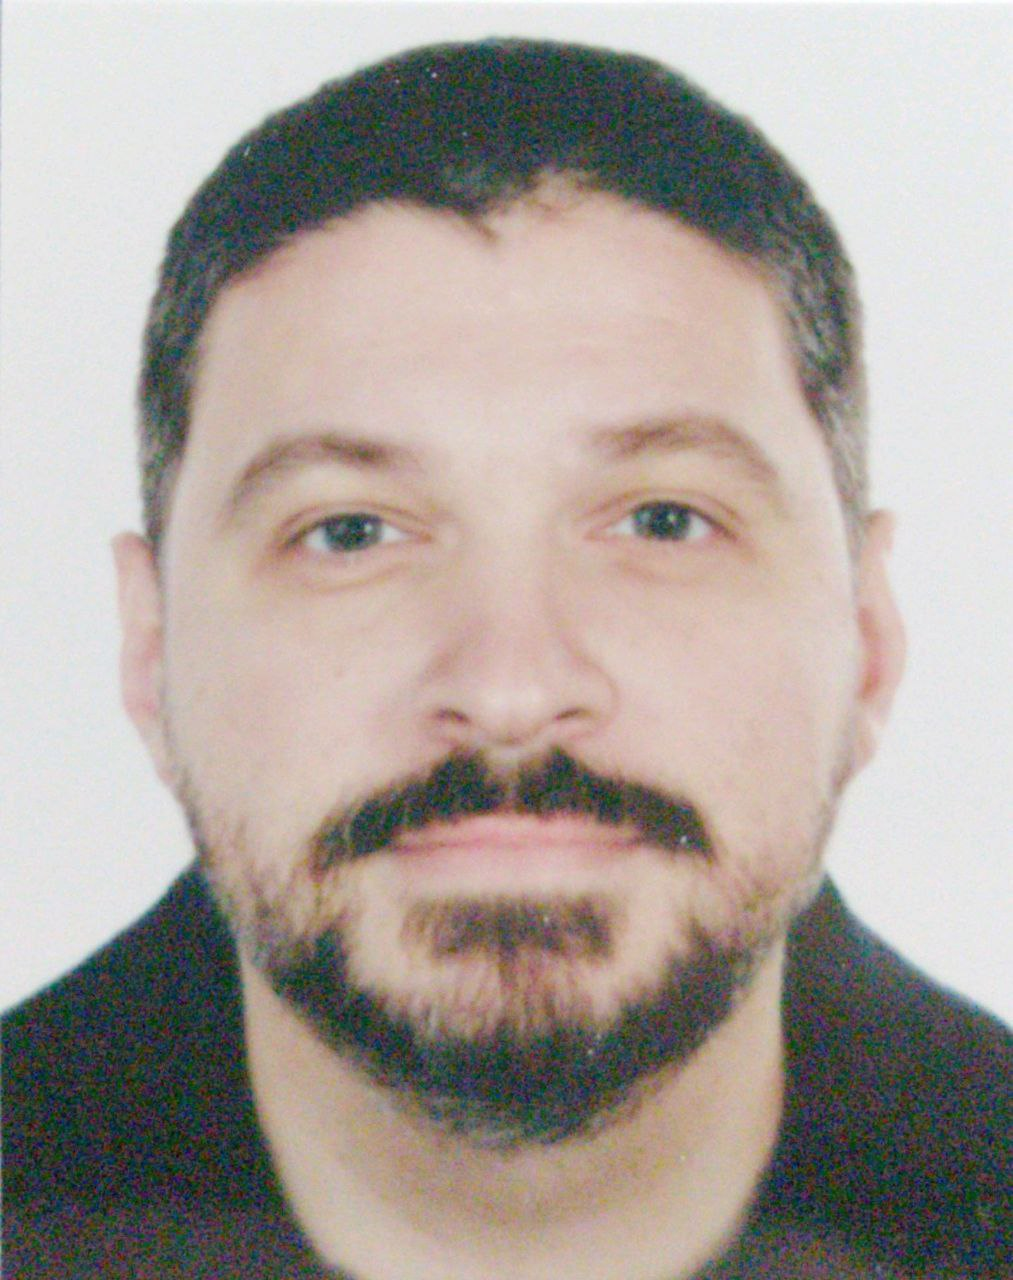
\includegraphics{author_photo.eps}
% IEEE Access accepts EPS, PDF or high-resolution PNG (square aspect).
\vspace{6pt}
\noindent
\begin{minipage}[t]{0.20\linewidth}
  \vspace{0pt}
  \rule{1.0in}{1.25in}\par
  \vspace{2pt}
  \footnotesize{photo placeholder}
\end{minipage}\hfill
\begin{minipage}[t]{0.78\linewidth}
  \vspace{0pt}
  \textbf{Oleksandr Kalynovskyi} is an independent researcher working on
  fault-tolerant distributed systems for autonomous aerial vehicles, with
  a focus on Byzantine-resilient cooperative navigation, factor-graph
  state estimation under GNSS denial, and reproducible empirical
  validation of swarm protocols in physics-grounded simulation. The work
  reported in this paper was carried out independently; the methods of
  Sections~\ref{sec:approach}-B through~\ref{sec:approach}-G are the
  subject of pending patent applications filed in April~2026 at the
  German Patent and Trademark Office (DPMA), Aktenzeichen
  10~2026~001~712.2 and a related filing. The author maintains the open
  \texttt{uav-gazebo-lab} reproducibility repository
  (Section~\ref{sec:code-data}) and welcomes correspondence regarding
  empirical replication, baseline-protocol comparison campaigns, and
  hardware-in-the-loop extensions of the present results.
\end{minipage}

\end{document}
